\documentclass[a4paper,12pt,twoside]{book}
\usepackage{upatras-thesis}


% PDF settings
%
% \hypersetup
% {
%     pdfauthor={\me},
%     pdftitle={\shortdoctitle},
%     pdfsubject={\doctitle},
%     pdfkeywords={\keywords},
%     pdfproducer={pdfLaTeX},
%     pdfcreator={\creator}
% }

%
% These commands need to be defined in order to produce a correct and personalized document
%
\newcommand{\shortdoctitle}{Διπλωματική Εργασία}
\newcommand{\doctitle}{Σύστημα Υποβοήθησης Πλοήγησης για Άτομα με Προβλήματα Όρασης}
% \newcommand{\docsubtitle}{Υπότιτλος εγγράφου}
\newcommand{\division}{Τηλεπικοινωνιών και Τεχνολογίας Πληροφορίας (Τ.\&Τ.Π.)}
\newcommand{\lab}{Ομάδα Απεικόνισης Πληροφορίας \& Εικονικής Πραγματικότητας}

\newcommand{\me}{Ιωάννη Κουτουλογένη του Ανδρέα} %(σε γενική πτώση) ΠΡΟΣΟΧΗ: στοιχεία σε γενική πτώση. Παράδειγμα: Άγγελου Σικελιανού του Ιωάννη
%
\newcommand{\nomme}{Ιωάννης Κουτουλογένης του Ανδρέα} %(σε ονομαστική πτώση) ΠΡΟΣΟΧΗ: στοιχεία σε ονομαστική πτώση. Παράδειγμα: Άγγελος Σικελιανός του Ιωάννη
%
\newcommand{\studnum}{1019659}
\newcommand{\keywords}{}
\newcommand{\monthyear}{Φεβρουάριος 2020}

\newcommand{\supname}{Κωνσταντίνος Μουστάκας}
\newcommand{\suptitle}{Αναπληρωτής Καθηγητής}
\newcommand{\supuni}{Πανεπιστήμιο Πατρών}

\newcommand{\cosupname}{Κυριάκος Σγάρμπας}
\newcommand{\cosuptitle}{Αναπληρωτής Καθηγητής}
\newcommand{\cosupuni}{Πανεπιστήμιο Πατρών}

\newcommand{\headofdivision}{Ιωάννης Μουρτζόπουλος}
\newcommand{\headofdivisiontitle}{Καθηγητής}

\author{\me}

% GLOSSARY

\makeglossaries
\setlength{\glsdescwidth}{0.7\hsize}
\setlength{\headheight}{15pt}
%\newglossaryentry{iot-connection}
%{name=IoT Connection, description={ In the proposed system architecture each child layer is “managed” by the parent layer. A connection indicates this management relationship between two devices (e.g cloud-edge) that belong to different layers.}}

\newglossaryentry{ui}{
    name=Διεπαφή Χρήστη (User Interface), 
    description={mpla mpla mpla...}
}
\newglossaryentry{ui}{
    name=Απτική Ανάδραση (Haptic Feedback), 
    description={mpla mpla mpla...}
}

\newglossaryentry{SDK}{
    name=Απτική Ανάδραση (Haptic Feedback), 
    description={mpla mpla mpla...}
}
\newglossaryentry{OpenCV}{
    name=Απτική Ανάδραση (Haptic Feedback), 
    description={mpla mpla mpla...}
}

\newglossaryentry{IDE}{
    name=Απτική Ανάδραση (Haptic Feedback), 
    description={mpla mpla mpla...}
}

\newacronym{who}{ΠΟΥ}{Παγκόσμιος Οργανισμός Υγείας}
\newacronym{eta}{ETAs}{Electronic Travel Aids}
\newacronym{gps}{GPS}{Global Positioning System}
\newacronym{rfid}{RFID}{Radio Frequency IDentification}
\newacronym{ann-gr}{ΤΝΔ}{Τεχνητά Νευρωνικά Δίκτυα}
\newacronym{amea}{ΑμΕΑ}{Άτομα με Ειδικές Ανάγκες}

% BEGIN DOCUMENT
\begin{document}

% SET PAGE NUMBERING TO ROMAN
\pagenumbering{roman}
\setcounter{page}{3}

%*************************%
%         TITLES          %
%*************************%

\begin{titlepage}
\begin{center}
% Upper part of the page
\large{ΠΑΝΕΠΙΣΤΗΜΙΟ ΠΑΤΡΩΝ - ΠΟΛΥΤΕΧΝΙΚΗ ΣΧΟΛΗ}\\
\large{ΤΜΗΜΑ ΗΛΕΚΤΡΟΛΟΓΩΝ ΜΗΧΑΝΙΚΩΝ ΚΑΙ ΤΕΧΝΟΛΟΓΙΑΣ ΥΠΟΛΟΓΙΣΤΩΝ}\\
{Τομέας: \division \\
\lab}

\hfill \break

\includegraphics[width= 0.8\textwidth]{up_landscape}\\
\noindent\rule{15cm}{1pt}\\[1cm]

{\uline{\LARGE{\shortdoctitle }}}\\ [0.5cm]
του φοιτητή του Τμήματος Ηλεκτρολόγων Μηχανικών και Τεχνολογίας\\Υπολογιστών της Πολυτεχνικής Σχολής του Πανεπιστημίου Πατρών\\[1cm]

{\LARGE \me }\\[0.5cm]
{\Large αριθμός μητρώου: \studnum}\\[1cm]

\uline{\Large Θέμα}\\[0.5cm]
\textbf{\large \doctitle }\\[1cm]
\uline{\large Επιβλέπων}\\[0.5cm]
\large \supname\\
\suptitle, \supuni \\[1cm]
\large{Αριθμός Διπλωματικής Εργασίας: }\hspace{3cm}
\vfill
% Bottom of the page
\large{Πάτρα, \monthyear}
\end{center}
\end{titlepage}

\clearemptydoublepage

\pagestyle{empty}
\begin{center}
{\LARGE ΠΙΣΤΟΠΟΙΗΣΗ\\[1cm]}
\large Πιστοποιείται ότι η διπλωματική εργασία με θέμα\\[1cm]
\textbf{\large \doctitle }\\[1cm]
του φοιτητή του Τμήματος Ηλεκτρολόγων Μηχανικών και Τεχνολογίας Υπολογιστών\\[1.5cm]
\me \\[0.5cm]
Αριθμός Μητρώου: \studnum \\[1.5cm]
παρουσιάστηκε δημόσια και εξετάστηκε στο τμήμα  Ηλεκτρολόγων Μηχανικών και Τεχνολογίας Υπολογιστών στις\\[0.5cm]
\text{20/02/2020}\\[2.5cm]
\end{center}
\begin{minipage}{0.5\textwidth}
\begin{flushleft} \large
Ο Επιβλέπων\\[0.5cm]
\supname \\
\emph{\suptitle}
\end{flushleft}
\end{minipage}
\begin{minipage}{0.5\textwidth}
\begin{flushright} \large
Ο Διευθυντής του Τομέα\\[0.5cm]
\headofdivision\\
\emph{\headofdivisiontitle}
\end{flushright}
\end{minipage}\\
\begin{minipage}{\textwidth}
\begin{flushleft} \large
\vfill\null
\vfill\null
\vfill\null
\vfill\null
\end{flushleft}
\end{minipage}
%\begin{minipage}{0.5\textwidth}
%\begin{flushleft} \large
%Ο Συνεξεταστής\\[0.5cm]
%\cosupname \\
%\emph{\cosuptitle}
%\end{flushleft}
%\end{minipage}

\clearemptydoublepage

% \pagestyle{empty}
\begin{center}
{\LARGE CERTIFICATION\\[1cm]}
\large It is certified that the Thesis with Subject\\[1cm]
\textbf{\large \doctitle }\\[1cm]
of the student of the Department of Electrical Engineering \& Computer Technology\\[1.5cm]
\me \\[0.5cm]
(R.N: \studnum )\\[1.5cm]
Was presented publicly and defended at the Department of Electrical Engineering \& Computer Technology at\\[1cm]
\Large{\_\_/\_\_/\_\_\_}\\[1.5cm]
\end{center}
\begin{minipage}{0.5\textwidth}
\begin{flushleft} \large
The Supervisor\\[2cm]
\supname \\
\emph{\suptitle}\\[1cm]
The Co-Supervisor\\[2cm]
\cosupname
\emph{\cosuptitle}

\end{flushleft}
\end{minipage}
\begin{minipage}{0.5\textwidth}
\begin{flushright} \large
The Director of the Division\\[4cm]
\headofdivision\\
\emph{\headofdivisiontitle}
\end{flushright}
\end{minipage}

% \clearemptydoublepage

% \pagestyle{empty}
\hspace{10pt}
\begin{center}
\Large{Thesis details}\\[1cm]
{\large Τίτλος:}
\textbf{\large \doctitle}\\[1cm]
\large {Φοιτητής: \textbf{\nomme}\\[1cm]
\large{Supervising Team}\\
\textbf{\suptitle \, \supname , \supuni}\\[1cm]
\textbf{\cosuptitle \, \cosupname , \cosupuni} \\[1cm]
Laboratories:\\
\lab \\[1cm]
Thesis research period:\\ July 2019 - January 2020\\[1cm]}
\end{center}

\vspace{5em}

\begin{center}
  { \large
    This thesis was written in \LaTeX.\\
  }
\end{center}


% \clearemptydoublepage

\pagestyle{plain}
\begin{center}
{\LARGE Περίληψη}\\[1cm]
\end{center}

Η παρούσα διπλωματική εργασία έχει ως αντικείμενο τον σχεδιασμό ενός ολοκληρωμένου και διακριτικού συστήματος πλοήγησης για άτομα με προβλήματα όρασης, το οποίο θα λειτουργεί συνδυαστικά με παραδοσιακά βοηθήματα, όπως είναι το λευκό μπαστούνι, και θα παρέχει στον χρήστη την δυνατότητα ασφαλέστερης και γρηγορότερης μετακίνησης μέσα σε ένα αστικό περιβάλλον, εστιάζοντας περισσότερο στο πρόβλημα διάσχισης ενός δρόμου μέσω μιας διάβασης πεζών. Στόχος είναι η υλοποίηση μιας πειραματικής διάταξης η οποία θα είναι πλήρως λειτουργική, θα αυξάνει το βαθμό αυτονομίας του χρήστη και θα βασίζεται πάνω σε 3 βασικούς άξονες: την φορητότητα, την ελάχιστη επεμβατικότητα και την αξιοπιστία. Για την εξασφάλιση των παραπάνω χαρακτηριστικών χρησιμοποιήθηκαν τεχνικές επεξεργασίας εικόνας και αναπτύχθηκαν 3 διαφορετικοί αλγόριθμοι, που αφορούν την ανίχνευση διάβασης πεζών, την αναγνώριση της κατάστασης των φωτεινών σηματοδοτών και τον εντοπισμό εμποδίων, καθώς επίσης και μια εφαρμογή για Android smartphones, η οποία αναλαμβάνει την καθοδήγηση και αποτελεί την διεπιφάνεια αλληλεπίδρασης μεταξύ του συστήματος και του χρήστη. Η παροχή ανάδρασης στον χρήστη πραγματοποιείται μέσω του smartphone και τη χρήση 4 διαφορετικών μοτίβων δονήσεων, με σκοπό την αξιοποίηση του απτικού καναλιού και την αποσυμφόρηση του ακουστικού καναλιού του χρήστη. Η τελική πειραματική διάταξη περιλαμβάνει την ενσωμάτωση μιας κάμερας με αισθητήρα βάθους, ενός μικροϋπολογιστή, μιας φορητής μπαταρίας τύπου power bank και ένα smartphone.
\pagestyle{plain}
\begin{center}
{\LARGE Abstract}\\[1cm]
\end{center}

The current diploma thesis addresses the problem of designing a complete and discreet navigational system for visually impaired people, supporting the traditional assisting methods like white cane and providing the user with the ability to move safer and faster throughout an urban environment, especially when it comes to crossing a road through a crosswalk. The ultimate goal is to implement an experimental setup that will be totally functional, will increase user's autonomy and will follow 3 main principles; portability, low intrusiveness and reliability. For satisfying the above criteria we made use of diverse image processing techniques and developed 3 different algorithms, for crosswalk detection, for pedestrian lights recognition and for obstacle detection, while also developing an Android application, which is responsible for the guidance and the interaction between the system and the user. The feedback to the user is provided through his smartphone, by using 4 different vibration patterns, because we wanted to utilize the haptic channel and limit the cognitive load connected with the acoustic channel. The final experimental setup includes the incorporation of a camera with a depth sensor, a microcomputer, a portable battery (power bank) and a smartphone.
\clearemptydoublepage

\begin{center}
{\LARGE Ευχαριστίες}\\[1cm]
\end{center}

Ολοκληρώνοντας την διπλωματική μου εργασία, δεν μπορώ παρά να ευχαριστήσω τα άτομα που διαδραμάτισαν καθοριστικό ρόλο στην πορεία των φοιτητικών μου χρόνων και την επιτυχή περάτωση των σπουδών μου.

Καταρχάς, θα ήθελα να ευχαριστήσω θερμά τον επιβλέποντα καθηγητή της διπλωματικής μου εργασίας κ. Κωνσταντίνο Μουστάκα για τις συνεχείς συμβουλές και την πολύτιμη καθοδήγησή του καθ' όλη την διάρκεια εκπόνησης της εργασίας, καθώς επίσης και για την θετική ενέργεια την οποία μου μετέδιδε σε κάθε μας συνάντηση.

Παράλληλα, θα ήθελα να ευχαριστήσω από καρδιάς τα μέλη και το ερευνητικό προσωπικό της ομάδας Απεικόνισης Πληροφορίας \& Εικονικής Πραγματικότητας για τις ώρες και τα σαββατοκύριακα που περάσαμε μαζί τους τελευταίους μήνες, ενώ ιδιαίτερη αναφορά θα ήθελα να κάνω στους Γιώργο Μιχαλάκη, Σωτήρη Αλεξίου και Άγγελο Χατζηκαλύμνιο για την συνεισφορά τους στην υλοποίηση του βίντεο επίδειξης της διπλωματικής μου εργασίας.

Τέλος, νιώθω την ανάγκη να ευχαριστήσω την οικογένειά μου για την αγάπη και τη στήριξη που μου παρείχε καθ' όλη την διάρκεια των σπουδών μου, όπως επίσης και τους φίλους μου που ήταν πάντα δίπλα μου και με ενέπνευσαν ο καθένας με τον τρόπο του.\\[2cm]

\begin{flushright}
    \emph{Στην γιαγιά μου,\\
    για την αμέριστη συμπαράστασή της\\
    όλα αυτά τα χρόνια}
\end{flushright}
\clearemptydoublepage

\pagestyle{empty}

{\hypersetup{linkcolor=black}
\renewcommand*\contentsname{Περιεχόμενα}
\tableofcontents
}
\clearemptydoublepage

%*************************%
%    1. Lists of figures  %
%    2. List of Tables    %
%    3. Glossary          %
%*************************%
% \listoffigures
% \listoftables
% \printglossaries
% \clearemptydoublepage

{\hypersetup{linkcolor=black}
\listoffigures
\listoftables
\glsaddall
%\printglossary[title=Ακρωνύμια, toctitle=Ακρωνύμια,type=\acronymtype] % prints just the list of acronyms
\clearemptydoublepage
%\printglossary[style = mylong]
}

%\printglossary
% \clearemptydoublepage

% easter_egg

\mainmatter % book mode only
\clearemptydoublepage


\pagestyle{fancy}
\pagenumbering{arabic}
\setcounter{page}{1}

%*************************%
%       Main Chapters     %
%*************************%

% Introduction
%!TEX root = ../main.tex

\chapter{Εισαγωγή}
\markboth{Εισαγωγή}{}

Στο κεφάλαιο αυτό γίνεται μια εισαγωγή στην κατάσταση που επικρατεί γύρω από τα άτομα με προβλήματα όρασης. Πιο συγκεκριμένα, παρατίθενται ορισμένα στατιστικά στοιχεία σχετικά με τον αριθμό των ατόμων με μειωμένη όραση, δίνεται ένας ορισμός της έννοιας της τύφλωσης και παρουσιάζονται μερικές από τις δυσκολίες που αναγκάζεται να αντιμετωπίσει ένα τέτοιο άτομο κατά την πλοήγησή του σε μια πόλη. Τέλος, αναφέρονται τα κίνητρα τα οποία με οδήγησαν στην συγγραφή αυτής της διπλωματικής εργασίας, ενώ παράλληλα δίνεται μια σύντομη περιγραφή των κεφαλαίων που την συνθέτουν.

\section{Στατιστικά στοιχεία για άτομα με προβλήματα όρασης}
Για να προχωρήσουμε στον σχεδιασμό ενός συστήματος πλοήγησης για τα άτομα με προβλήματα όρασης, πρέπει πρώτα να λάβουμε υπόψιν την κατηγοριοποίηση των ατόμων αυτών με βάση το ποσοστό τύφλωσής τους. Ο Παγκόσμιος Οργανισμός Υγείας (\url{https://www.who.int}), ο οποίος είναι ο πλέον αξιόπιστος φορέας σε θέματα που αφορούν την παγκόσμια υγεία, ορίζει την τύφλωση ως την μειωμένη ικανότητα όρασης σε βαθμό τέτοιο, ώστε τα προβλήματα δεν μπορούν να διορθωθούν με οποιοδήποτε μέσο, π.χ. γυαλιά, και παράλληλα προτείνει την ταξινόμηση των επιπέδων όρασης σε 4 βασικές κατηγορίες \cite{world_health_organization}:
\begin{itemize}
    \item Φυσιολογική όραση – Normal vision
    \item Μέτρια Διαταραχή όρασης – Moderate visual impairment
    \item Σοβαρή Διαταραχή όρασης – Severe visual impairment
    \item Ολική Απώλεια όρασης – Blindness
\end{itemize}

Σύμφωνα με μια έρευνα που δημοσιεύτηκε το 2017 \cite{bourne2017magnitude} το ποσοστό των ατόμων που παρουσιάζουν κάποιο πρόβλημα όρασης ή τύφλωση ανέρχεται στο 29,5\% επί του συνόλου του παγκόσμιου πληθυσμού, δηλαδή το 1/3 του πληθυσμού παρουσιάζει κάποια δυσλειτουργία στην όραση. Στη ίδια έρευνα αναφέρεται ότι 36 εκατομμύρια άνθρωποι πάσχουν από ολική τύφλωση, ενώ 217 εκατομμύρια παρουσιάζουν κάποιας μορφής σοβαρή ή ήπια πάθηση, ενώ αξίζει να σημειώσουμε ότι στις περισσότερες περιπτώσεις η απώλεια όρασης θα μπορούσε να είχε αποφευχθεί αν υπήρχε η κατάλληλη πρόληψη και διενέργεια οφθαλμολογικών εξετάσεων. Δεδομένου ότι το ποσοστό των ανθρώπων με κάποιας μορφής τύφλωση είναι υψηλότερο στις χώρες με μέτριο ή χαμηλό εισόδημα, καταλαβαίνουμε ότι η πρόληψη είναι άμεσα συνδεδεμένη με το βιοτικό επίπεδο των πολιτών και την οικονομική τους δυνατότητα για πρόσβαση σε ιατρική περίθαλψη.

\begin{figure}[H]
    \centering
    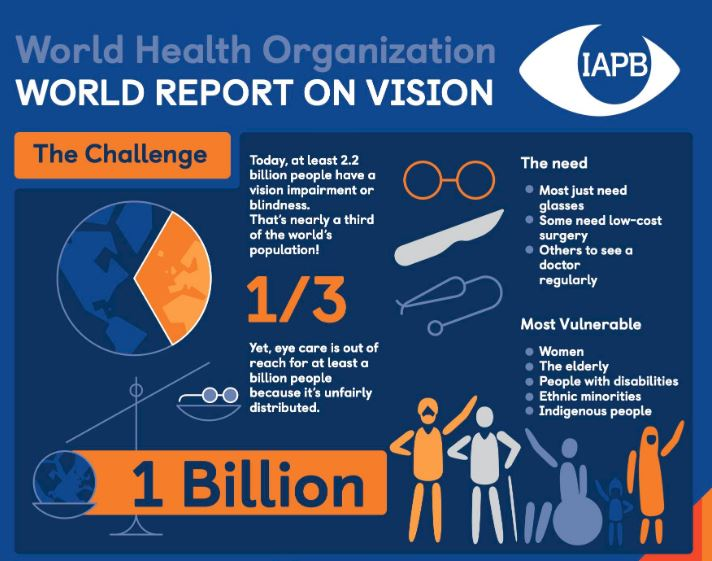
\includegraphics[width=0.8\textwidth]{images/who_stats.JPG}
    \caption{Έκθεση του Παγκόσμιου Οργανισμού Υγείας για τα ποσοστά ανθρώπων με προβλήματα όρασης \cite{Whatexac14:online}}
    \label{fig:who-stats}
\end{figure}

\section{Δυσκολίες πλοήγησης σε αστικά περιβάλλοντα}
Τα περισσότερα άτομα με προβλήματα όρασης επιλέγουν να ζήσουν σε πόλεις, επειδή η οργάνωση και οι δυνατότητες που τους παρέχονται είναι πολύ καλύτερες σε σύγκριση με τη ζωή στην ύπαιθρο. Παρ' όλα αυτά, ένα από τα μεγαλύτερα εμπόδια που αντιμετωπίζουν είναι αυτό της μετακίνησης. Η δυνατότητα αυτών των ατόμων να μετακινούνται αυτόνομα σε ένα αστικό περιβάλλον είναι αυτή που τους επιτρέπει να έχουν μια αξιοπρεπή ζωή, χωρίς αυτήν το βιοτικό τους επίπεδο μειώνεται δραματικά. Σύμφωνα με έρευνες που έχουν πραγματοποιηθεί σε αυτό το πεδίο \cite{riazi_outdoor_2016,parkin2012blind-needs}, μερικές από τις προκλήσεις που αντιμετωπίζουν τα άτομα με μειωμένη όραση είναι:
\begin{itemize}
    \item Συνεχής ανάγκη να ζητούν βοήθεια από περαστικούς
    \item Δυσκολία αναγνώρισης διαδρομών και χρήσης GPS
    \item Ρίσκο ατυχήματος
    \item Δυσκολία χρήσης των ανάγλυφων πλακιδίων για τυφλούς στα πεζοδρόμια
    \item Μη σωστή χρήση του λευκού μπαστουνιού οδηγεί σε ατυχήματα
    \item Φόβος χρήσης σκύλου-οδηγού
    \item Ελλιπής συντήρηση των πεζοδρομίων
    \item Απρόσεκτη συμπεριφορά πεζών
\end{itemize}

Ένα από τα σημαντικότερα προβλήματα μοιάζει να είναι η διάσχιση ενός δρόμου \cite{alwi2013survey}. Φανταστείτε τον εαυτό σας μπροστά από ένα μεγάλο σταυροδρόμι ή στην άκρη μιας μεγάλης λεωφόρου την οποία πρέπει να διασχίσετε. Ένα άτομο με μειωμένη όραση πρέπει να λάβει υπόψιν του πολλούς παράγοντες πριν ξεκινήσει να διασχίζει τον δρόμο, όπως για παράδειγμα την ύπαρξη ή όχι διάβασης πεζών, την ταχύτητα με την οποία πλησιάζουν τα διερχόμενα οχήματα, τυχόν εμπόδια που υπάρχουν κατά μήκος της διαδρομής του, καθώς επίσης και τον χρόνο τον οποίο χρειάζεται για να διασχίσει τον δρόμο.

Κατανοούμε λοιπόν την ανάγκη ύπαρξης καλύτερων υποδομών, σωστής και επαρκούς σήμανσης στους δρόμους, καθώς και την ανάγκη να γίνουμε πιο προσεκτικοί απέναντι στους συμπολίτες μας με μειωμένη όραση.

\section{Κίνητρα και σκοπός διπλωματικής εργασίας}
Ο βασικότερος λόγος που με ώθησε να ασχοληθώ με το συγκεκριμένο θέμα είναι η έλλειψη κατάλληλων προϋποθέσεων, ώστε τα άτομα με προβλήματα όρασης να έχουν ίσες ευκαιρίες στην καθημερινότητά τους και να μην περιορίζονται από το ποσοστό αναπηρίας που μπορεί να έχουν. Η καθημερινότητά μας καθορίζεται σε μεγάλο ποσοστό από το πόσο εύκολα μπορούμε να πραγματοποιήσουμε εργασίες αυτόνομα και ανεξάρτητα, χωρίς να βασιζόμαστε αποκλειστικά σε άλλους. Για τους πολίτες δίχως προβλήματα όρασης το να βγουν από το σπίτι τους και να μετακινηθούν μέχρι το πάρκο για μια βόλτα ή να περπατήσουν μέχρι το τοπικό σούπερ μάρκετ για τα ψώνια τους είναι κάτι το αυτονόητο και δεν αποτελεί επιπλέον κόπο. Αντιθέτως, για ένα άτομο με μειωμένη ή ολική απώλεια όρασης, ακόμα και το να βγει από το σπίτι του περπατώντας στην άκρη του πεζοδρομίου αποτελεί μια ενέργεια που ενέχει κινδύνους και απαιτεί έντονη συγκέντρωση και πνευματική προσπάθεια. Το δικαίωμα στην ελεύθερη, αυτόνομη και ασφαλή μετακίνηση είναι κάτι που θα έπρεπε να απολαμβάνουν όλοι οι άνθρωποι.

Η τεχνολογία σήμερα μας επιτρέπει να αλλάζουμε τον τρόπο με τον οποίο αντιμετωπίζουμε την πραγματικότητα και να δίνουμε λύσεις σε προβλήματα που είναι δύσκολα και περίπλοκα. Έχοντας υπόψιν τα παραπάνω, στόχος της παρούσας διπλωματικής εργασίας είναι ο σχεδιασμός και η υλοποίηση ενός συστήματος υποβοήθησης πλοήγησης που θα επιτρέπει στους χρήστες με προβλήματα όρασης να κινούνται με περισσότερη άνεση μέσα σε ένα αστικό περιβάλλον, συμβάλλοντας έτσι στην αύξηση της αυτονομίας τους. Θα πρέπει να τονιστεί ότι το προτεινόμενο σύστημα στόχο έχει να ενισχύσει την λειτουργία του λευκού μπαστουνιού, που χρησιμοποιείται κατά κόρον από τους τυφλούς, και όχι να την αντικαταστήσει. Παράλληλα, η παρούσα εργασία εστιάζει κυρίως στην παροχή βοήθειας στους χρήστες για την αποτελεσματικότερη και ασφαλέστερη διάσχιση μιας διάβασης πεζών, ενώ αξίζει να τονιστεί ότι η παροχή ανατροφοδότησης στον χρήστη κατά την πλοήγηση δίνεται μέσω της αφής, με σκοπό την αξιοποίηση του απτικού καναλιού και την μείωση του φόρτου στο κανάλι της ακοής.

\section{Διάρθρωση διπλωματικής εργασίας}
Έχοντας επίγνωση των αναγκών και της πολυπλοκότητας ενός συστήματος πλοήγησης για άτομα με προβλήματα όρασης, έχει γίνει προσπάθεια να παρουσιαστούν με τον πιο κατανοητό και περιεκτικό τρόπο όλες οι πλευρές ενός τέτοιου συστήματος. Για τον λόγο αυτό η παρούσα εργασία διαμορφώνεται ως εξής:
\begin{itemize}
    \item Στο κεφάλαιο 2 «\nameref{ch:state-of-the-art}» γίνεται αναφορά στην προγενέστερη έρευνα που έχει γίνει στο αντίστοιχο ερευνητικό πεδίο. Πιο συγκεκριμένα, παρουσιάζονται τα βοηθητικά μέσα που έχουν στη διάθεσή τους τα άτομα με δυσκολία όρασης, γίνεται διαχωρισμός των ηλεκτρονικών συστημάτων υποβοήθησης πλοήγησης σε τρεις κύριες κατηγορίες και τέλος παρατίθενται μερικά από τα πιο αντιπροσωπευτικά συστήματα πλοήγησης εξωτερικού χώρου που έχουν αναπτυχθεί.
    \item Στο κεφάλαιο 3 «\nameref{ch:system-architecture}» γίνεται μια αναλυτική περιγραφή της αρχιτεκτονικής του προτεινόμενου συστήματος, των ελάχιστων προδιαγραφών ενός συστήματος πλοήγησης για άτομα με προβλήματα όρασης και παρουσιάζονται με λεπτομέρεια τα διάφορα μέρη που χρησιμοποιήθηκαν για την υλοποίησή του. 
    \item Στο κεφάλαιο 4 «\nameref{ch:demo}» παρουσιάζεται ο τρόπος με τον οποίο έγινε ο πειραματικός έλεγχος της ορθής λειτουργίας του συστήματος και αναφέρονται τα διάφορα αποτελέσματα που προέκυψαν.
    \item Στο κεφάλαιο 5 «\nameref{ch:conclusion}» αναλύονται τα πλεονεκτήματα και τα μειονεκτήματα του προτεινόμενου συστήματος και παρατίθενται διάφορες προτάσεις για την βελτίωση της αποδοτικότητάς του.
\end{itemize}
\clearemptydoublepage
% % Chapters
\chapter{Προγενέστερη έρευνα στο πεδίο} \label{ch:state-of-the-art}
\markboth{Προγενέστερη έρευνα στο πεδίο}{}

Για πολλά χρόνια οι άνθρωποι προσπαθούσαν να βρουν λύσεις που θα βελτίωναν την καθημερινότητα των ατόμων με μειωμένη όραση. Ο κύριος στόχος κάθε τέτοιας προσπάθειας ήταν να καταστήσουν πιο ασφαλή την πλοήγηση του χρήστη στον χώρο και παράλληλα να αυξήσουν την ταχύτητα με την οποία ο τυφλός χρήστης λαμβάνει αποφάσεις κατά τη διάρκεια της πλοήγησής του. Στο κεφάλαιο αυτό γίνεται μια αναδρομή, ξεκινώντας από τις κλασικές μεθόδους πλοήγησης των ατόμων με μειωμένη όραση μέχρι και τις πιο σύγχρονες ηλεκτρονικές συσκευές υποβοήθησης ταξιδιού (ETAs). Επιπλέον, παρουσιάζεται η τρέχουσα τάση στο σχετικό ερευνητικό πεδίο και παρατίθενται οι διάφορες κατηγορίες των συστημάτων υποβοήθησης πλοήγησης.

\section{Βοηθητικά μέσα υποστήριξης ατόμων με μειωμένη όραση}
Εδώ και εκατοντάδες χρόνια οι άνθρωποι χρησιμοποιούσαν διάφορα μέσα με σκοπό την καθοδήγηση των ατόμων με μειωμένη όραση. Τα πιο διαδεδομένα και ευρέως αποδεκτά από την κοινότητα των τυφλών είναι το λευκό μπαστούνι και ο σκύλος οδηγός \cite{social_sciences_libguides_nodate}. Τις τελευταίες δεκαετίες, μετά την ραγδαία άνοδο της τεχνολογίας, ήρθαν στο προσκήνιο νέες συσκευές υποβοήθησης πλοήγησης που "σκανάρουν" το εξωτερικό περιβάλλον και μεταδίδουν την πληροφορία αυτή στον τυφλό μέσω ηχητικών ή απτικών σημάτων.
\subsection{Συμβατικά μέσα καθοδήγησης}
Πρόκειται για τα μέσα που χρησιμοποιούνται κατά κόρον από τα άτομα με περιορισμένη όραση. Τα μέσα αυτά έχουν αποδειχθεί πολύ χρήσιμα στην καθημερινότητα των τυφλών, έχουν κερδίσει την εμπιστοσύνη της κοινότητας αυτής, αλλά πολύ συχνά η περιορισμένη ελευθερία κινήσεων που επιτρέπουν ή το κόστος τους αποτελούν ανασταλτικούς παράγοντες για την απόκτησή τους.
\subsubsection{Λευκό μπαστούνι}
Το λευκό μπαστούνι είναι ίσως το πιο διαδεδομένο μέσο καθοδήγησης των τυφλών. Προσφέρει αυτονομία και αίσθηση ασφάλειας στον χρήστη, καθώς του επιτρέπει να σκανάρει τον περιβάλλοντα χώρο και να εντοπίζει τυχόν εμπόδια ή επιφάνειες προσανατολισμού, με περιορισμένο ωστόσο εύρος κινήσεων. Παράλληλα, η χρήση του επιτρέπει στους υπόλοιπους περαστικούς να αναγνωρίσουν την ιδιότητα του τυφλού και συνεπώς να είναι πιο προσεκτικοί. Το λευκό του χρώμα έχει νομοθετηθεί και αποτελεί ένδειξη ότι το άτομο που το κρατάει έχει προβλήματα όρασης.
\begin{table}[H]
    \centering
    \begin{tabular}{|c|c|}
        \hline
        Θετικά & Αρνητικά \\
        \hline
        \hline
        Εύκολη χρήση & Περιορισμένο εύρος κινήσεων \\
        Φορητό & Αδυναμία αναγνώρισης του είδους του εμποδίου\\
        Χαμηλό κόστος & \\ 
        \hline
    \end{tabular}
    \caption{Λευκό μπαστούνι, θετικά και αρνητικά}
    \label{tab:white-cane}
\end{table}

\begin{figure}[H]
    \centering
    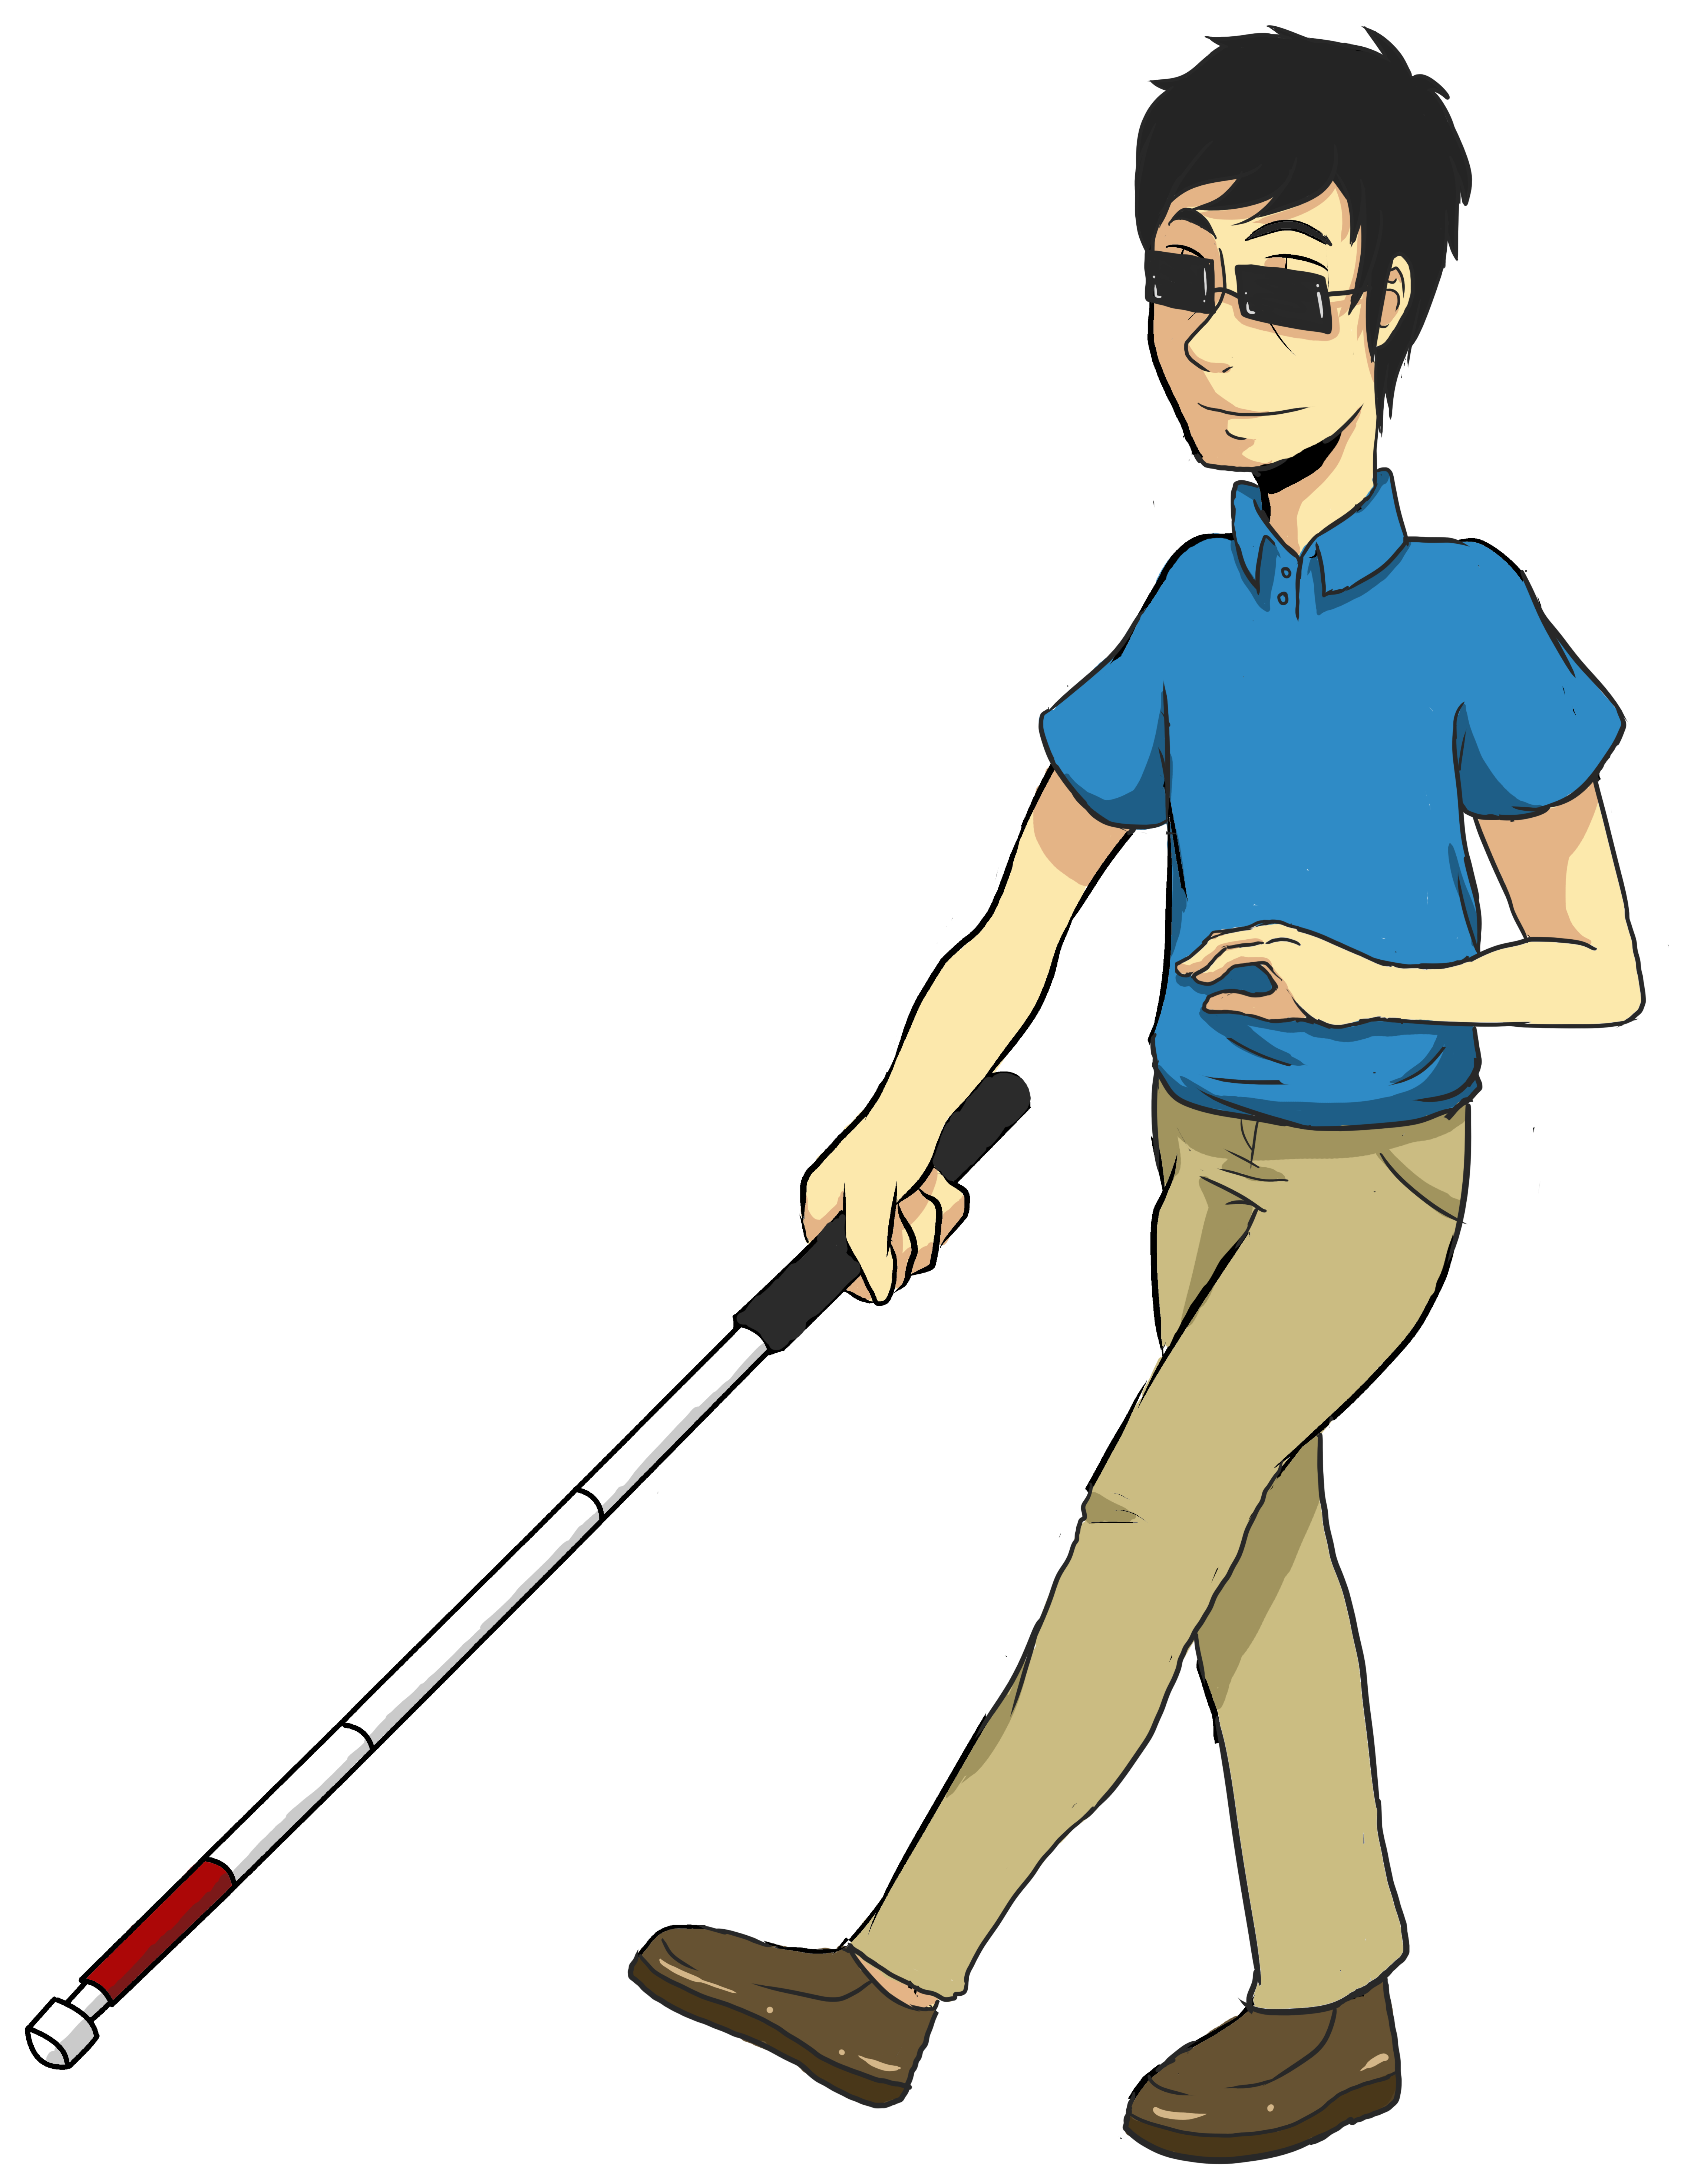
\includegraphics[width=0.4\textwidth]{images/white_cane_use.png}
    \caption{Παράδειγμα χρήσης λευκού μπαστουνιού}
    \label{fig:white-cane-use}
\end{figure}

\subsubsection{Σκύλος οδηγός}
Για πολλούς χρήστες με προβλήματα όρασης ο σκύλος οδηγός αποτελεί την καλύτερη λύση, αφού συνδυάζει την αίσθηση της ασφάλειας στην μετακίνηση με την αίσθηση της συντροφικότητας. Ο σκύλος οδηγός είναι εκπαιδευμένος να καθοδηγεί τον τυφλό με ασφάλεια, να αποφεύγει εμπόδια και να εντοπίζει στοιχεία όπως διαβάσεις, πόρτες, σκάλες, ταμεία και μέσα μαζικής μεταφοράς (π.χ., την είσοδο στο λεωφορείο). Η καθοδήγηση από έναν σκύλο οδηγό είναι πιο γρήγορη σε σύγκριση με το λευκό μπαστούνι, προσφέροντας μεγαλύτερη αυτονομία στον χρήστη. Παρ' όλα αυτά η εκπαίδευση ενός σκύλου οδηγού διαρκεί αρκετούς μήνες και απαιτεί αρκετούς οικονομικούς πόρους.
\begin{table}[H]
    \centering
    \begin{tabular}{|c|c|}
        \hline
        Θετικά & Αρνητικά \\
        \hline
        \hline
        Ασφάλεια & Υψηλό κόστος αγοράς\\
        Ταχύτητα & Κόστος συντήρησης\\
        Συντροφικότητα & Ανάγκη εκπαίδευσης σκύλου\\ 
        \hline
    \end{tabular}
    \caption{Σκύλος οδηγός, θετικά και αρνητικά}
    \label{tab:guide-dog}
\end{table}
\begin{figure}[h]
    \centering
    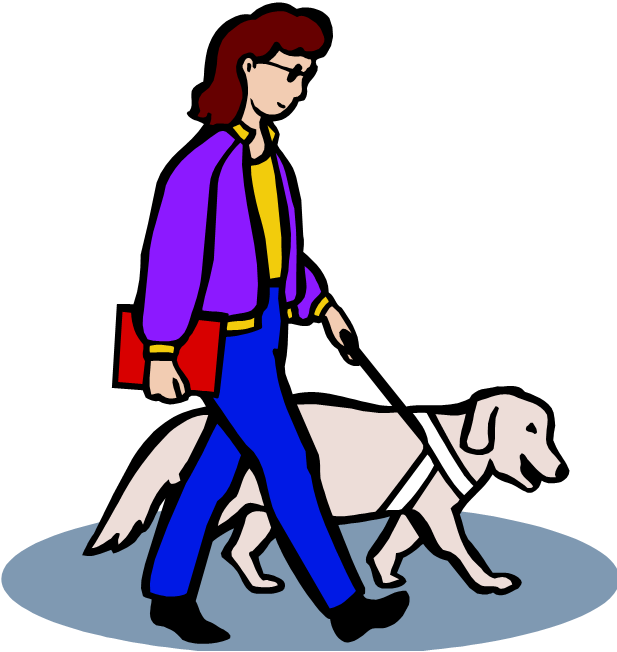
\includegraphics{images/guide_dog.png}
    \caption{Σκύλος οδηγός}
    \label{fig:guide-dog}
\end{figure}

\subsection{Ηλεκτρονικές συσκευές υποβοήθησης ταξιδιού (ETAs)}
Όσο η τεχνολογία προχωρούσε με ραγδαίους ρυθμούς και η υπολογιστική ισχύς γινόταν όλο και πιο μεγάλη, έκαναν την εμφάνισή τους οι λεγόμενες ηλεκτρονικές συσκευές υποβοήθησης ταξιδιού ή αλλιώς ΕΤΑs (Electronic Travel Aids). Αν και τα πρώτα χρόνια εμφάνισής τους οι ETAs επικεντρώνονταν κυρίως στην ανίχνευση και αποφυγή εμποδίων, τα τελευταία χρόνια έχουν αναπτυχθεί επαρκώς ώστε να υποστηρίζουν πλήρη περιγραφή των εμποδίων, της διαδρομής του χρήστη αλλά και συνεχή ανάδραση. Οι ερευνητές που ασχολούνται με την ανάπτυξη αυτών των συσκευών αξιοποιούν τις πληροφορίες που λαμβάνουν από το περιβάλλον γύρω από τον χρήστη και χρησιμοποιώντας συγκεκριμένες τεχνικές τον ειδοποιούν για τυχόν εμπόδια ή για την διαδρομή που πρέπει να ακολουθήσει.
\subsubsection{Αντίληψη περιβάλλοντος}
Οι άνθρωποι χρησιμοποιούν τα διάφορα αισθητήρια κανάλια για να κατανοήσουν το περιβάλλον γύρω τους. Όταν μιλάμε για πλοήγηση σε έναν χώρο τότε το κύριο αισθητήριο κανάλι που χρησιμοποιείται είναι αυτό της όρασης. Τα άτομα με μειωμένη ή καθόλου όραση τείνουν να αντικαθιστούν το οπτικό κανάλι με αυτό της ακοής ή της αφής. Συνήθως, το ακουστικό κανάλι είναι αυτό που χρησιμοποιείται κατά κύριο λόγο για να προσανατολιστούν και να αναγνωρίσουν τυχόν εμπόδια. Επιπρόσθετα, το απτικό κανάλι αξιοποιείται σε περίπτωση που τα άτομα αυτά θέλουν να κατανοήσουν με μεγαλύτερη λεπτομέρεια ένα εμπόδιο-αντικείμενο κοντά τους.

Επομένως, γίνεται κατανοητό ότι για να μπορέσουν οι ΕΤΑs να υποστηρίξουν τα άτομα με προβλήματα όραση πρέπει αρχικά να είναι σε θέση να αντιληφθούν το περιβάλλον γύρω τους με επιτυχία και ακρίβεια. Τον ρόλο των ματιών παίζουν οι διάφοροι τύποι αισθητήρων, όπως οι αισθητήρες υπερήχων, τα ραντάρ και οι κάμερες. Με χρήση αισθητήρων όπως αυτοί των υπερήχων το σύστημα είναι δυνατό να εντοπίσει ένα εμπόδιο μέχρι κάποια ορισμένη απόσταση, χωρίς ωστόσο να δώσει απάντηση σχετικά με την μορφολογία του. Από την άλλη μεριά, η χρήση κάμερας δίνει την δυνατότητα για πλήρη καταγραφή του περιβάλλοντος και με κατάλληλη επεξεργασία της εικόνας ή χρήση τεχνικών μηχανικής μάθησης μπορεί να δώσει απαντήσεις σχετικά με την μορφολογία των εμποδίων, την απόστασή τους, την υφή τους και το βέλτιστο μονοπάτι που μπορεί να ακολουθήσει ο χρήστης. Περισσότερα για τις κατηγορίες των συστημάτων πλοήγησης ανάλογα τον τρόπο "αίσθησης" του περιβάλλοντος θα αναλυθούν παρακάτω.
\subsubsection{Ανάδραση με χρήση ηχητικών ειδοποιήσεων}
Πέρα από την "αίσθηση" και την καταγραφή του περιβάλλοντος, ένα σύστημα πλοήγησης για άτομα με μειωμένη όραση θα πρέπει να μπορεί να μεταδώσει την οπτική πληροφορία στον χρήστη με αποδοτικό τρόπο. Επειδή όπως είπαμε και παραπάνω τα άτομα αυτά αξιοποιούν την αίσθηση της ακοής για τον προσανατολισμό τους τα περισσότερα ηλεκτρονικά συστήματα πλοήγησης χρησιμοποιούν το ακουστικό κανάλι για την μετάδοση της απαραίτητης πληροφορίας. Με άλλα λόγια, ο χρήστης ειδοποιείται μέσω ηχητικών σημάτων για την ύπαρξη κάποιου εμποδίου ή σε περίπτωση που υπάρχει ανάγκη για μια συγκεκριμένη δράση, όπως π.χ. να πραγματοποιήσει στροφή αριστερά/δεξιά ή να διασχίσει μια διάβαση πεζών. Τα ηχητικά αυτά σήματα μπορεί να είναι απλοί σύντομοι ή στιγμιαίοι ήχοι που ενημερώνουν τον χρήστη σχετικά με την απόσταση ενός εμποδίου, ή μπορεί να είναι σύντομες φράσεις/προτάσεις που να καθοδηγούν τον χρήστη σχετικά με την κατεύθυνση που πρέπει να ακολουθήσει.
\subsubsection{Ανάδραση με χρήση απτικών ειδοποιήσεων}
Πέρα από την ακοή, μια ακόμα αίσθηση που έχουν πολύ ανεπτυγμένη τα άτομα με προβλήματα όρασης είναι η αφή. Η αίσθηση της αφής είναι εκείνη που μας βοηθάει να αντιληφθούμε λεπτομέρειες σχετικά με τα αντικείμενα, όπως π.χ. την υφή των αντικειμένων. Τα τελευταία χρόνια έχει δοθεί ιδιαίτερη έμφαση στις συσκευές ΕΤΑs που βασίζονται στην ανάδραση με χρήση απτικών σημάτων, κυρίως επειδή ένα απτικό ερέθισμα είναι πολύ πιο διακριτικό σε σύγκριση με ένα ηχητικό και η αντίδραση του χρήστη σε αυτό είναι σχετικά πιο άμεση \cite{ng2012finger}. Οι διάφορες ETAs που έχουν κυκλοφορήσει κατά καιρούς χρησιμοποιούν ορισμένα μοτίβα δονήσεων για να ενεργοποιήσουν την αίσθηση της αφής στο χρήστη.



\section{Κατηγορίες συστημάτων υποβοήθησης πλοήγησης}
Η πλοήγηση ενός ατόμου μπορεί να διαιρεθεί σε δύο περιπτώσεις: α) πλοήγηση σε εσωτερικό χώρο, και β) πλοήγηση σε εξωτερικό χώρο. Και στις δύο περιπτώσεις για να έχουμε μια επιτυχημένη πλοήγηση είναι απαραίτητο να γνωρίζουμε τον προσανατολισμό που πρέπει να ακολουθήσει ο χρήστης, αλλά παράλληλα να ελέγχουμε ότι το μονοπάτι που ακολουθεί είναι ελεύθερο από εμπόδια. Συνεπώς, ένα ολοκληρωμένο σύστημα υποβοήθησης πλοήγησης για άτομα με μειωμένη όραση θα πρέπει να είναι σε θέση τόσο να παρέχει την κατεύθυνση του χρήστη σε σχέση με τον προορισμό του, όσο και να του εξασφαλίζει ένα ασφαλές μονοπάτι. 

Οι πρώτες συσκευές ETAs επικεντρώνονταν περισσότερο στο δεύτερο σκέλος, αυτό της αποφυγής εμποδίων, το οποίο επιτύγχαναν κυρίως με τη χρήση αισθητήρων υπερήχων ή σόναρ τα οποία εντόπιζαν ένα εμπόδιο σε μια συγκεκριμένη απόσταση και ειδοποιούσαν τον χρήστη για την ύπαρξη του. Με την ανάπτυξη της τεχνολογίας GPS (Global Positioning System) επήλθε και εντυπωσιακή πρόοδος όσον αφορά το πρώτο σκέλος των ETAs, αυτό της πλοήγησης. Το GPS λειτουργεί αξιοποιώντας την ύπαρξη 30+ δορυφόρων σε τροχιά γύρω από την γη, βάσει των οποίων μπορεί να εντοπίσει την τοποθεσία ενός δέκτη με ακρίβεια από μερικά μέτρα έως μερικά εκατοστά \cite{gps}. Η τεχνολογία αυτή επέτρεψε την κατασκευή συστημάτων πλοήγησης που όχι μόνο αναγνώριζαν πιθανά εμπόδια, αλλά μπορούσαν να κατευθύνουν τον χρήστη κατά την μετακίνησή του προς έναν προορισμό με αρκετά μεγάλη ακρίβεια. Ωστόσο, αν και το GPS λειτουργούσε αρκετά καλά στον εξωτερικό χώρο, η πλοήγηση στον εσωτερικό χώρο παρέμενε ακόμα ένα δύσκολο εγχείρημα, από την στιγμή που το σήμα του GPS εξασθενούσε σε μεγάλο βαθμό μέσα σε κτίρια. Για την αντιμετώπιση της πλοήγησης σε εσωτερικού χώρους έχουν δοθεί πολλαπλές λύσεις, με την πιο ενδιαφέρουσα από αυτές να αποτελεί η χρήση RFID (Radio Frequency IDentification), η οποία θα αναλυθεί παρακάτω. 

Τέλος, με την αύξηση της επεξεργαστικής ισχύος και την δυνατότητα κατασκευής όλο και μικρότερων επεξεργαστών τα συστήματα πλοήγησης, τόσο για εσωτερικούς όσο και για εξωτερικούς χώρους, άρχισαν πλέον να βασίζονται σε κάμερες και αισθητήρες βάθους. Παρακάτω παρουσιάζονται μερικά συστήματα πλοήγησης για άτομα με προβλήματα όρασης που έχουν αναπτυχθεί από προηγούμενες προσπάθειες ερευνητών. Έχει γίνει διαχωρισμός τους με βάση την τεχνολογία την οποία αξιοποιούν κατά κύριο λόγο για να πετύχουν την πλοήγηση του χρήστη ή την αναγνώριση των εμποδίων στην διαδρομή του.

\subsection{RFID}
Η τεχνολογία RFID, στα ελληνικά \textit{ταυτοποίηση μέσω ραδιοσυχνοτήτων}, αποτελεί την εξέλιξη των ραβδωτών κωδίκων barcode και χρησιμοποιείται ευρέως στην καθημερινή ζωή των ανθρώπων, κυρίως μέσω του εμπορίου. Ένα σύστημα RFID αποτελείται από δύο διαφορετικά μέρη:
\begin{enumerate}
    \item τον \textbf{πομποδέκτη}, οποίος συχνά αναφέρεται ως ετικέτα RFID (RFID tag) και
    \item τον \textbf{αναγνώστη ή αισθητήρα} (RFID reader).
\end{enumerate}

Ένα RFID tag αποτελείται από ένα εσωτερικό ολοκληρωμένο κύκλωμα το οποίο περιέχει μια κεραία για την επικοινωνία με τους RFID readers και μία μνήμη, στην οποία μπορούν να αποθηκευτούν διάφορα δεδομένα ή πληροφορίες για το αντικείμενο που φέρει την ετικέτα RFID. Ανάλογα την εφαρμογή στην οποία χρησιμοποιείται, η μνήμη μιας ετικέτας RFID μπορεί να είναι μόνο για ανάγνωση (\textit{Read Only Memory - ROM}), επανεγγράψιμη μνήμη (\textit{Read-Write Memory}), ή μνήμη μιας εγγραφής και πολλών αναγνώσεων (Write Once, Read Many - WORM) \cite{bonsor_fenlon_2007}.

\begin{figure}[H]
    \centering
    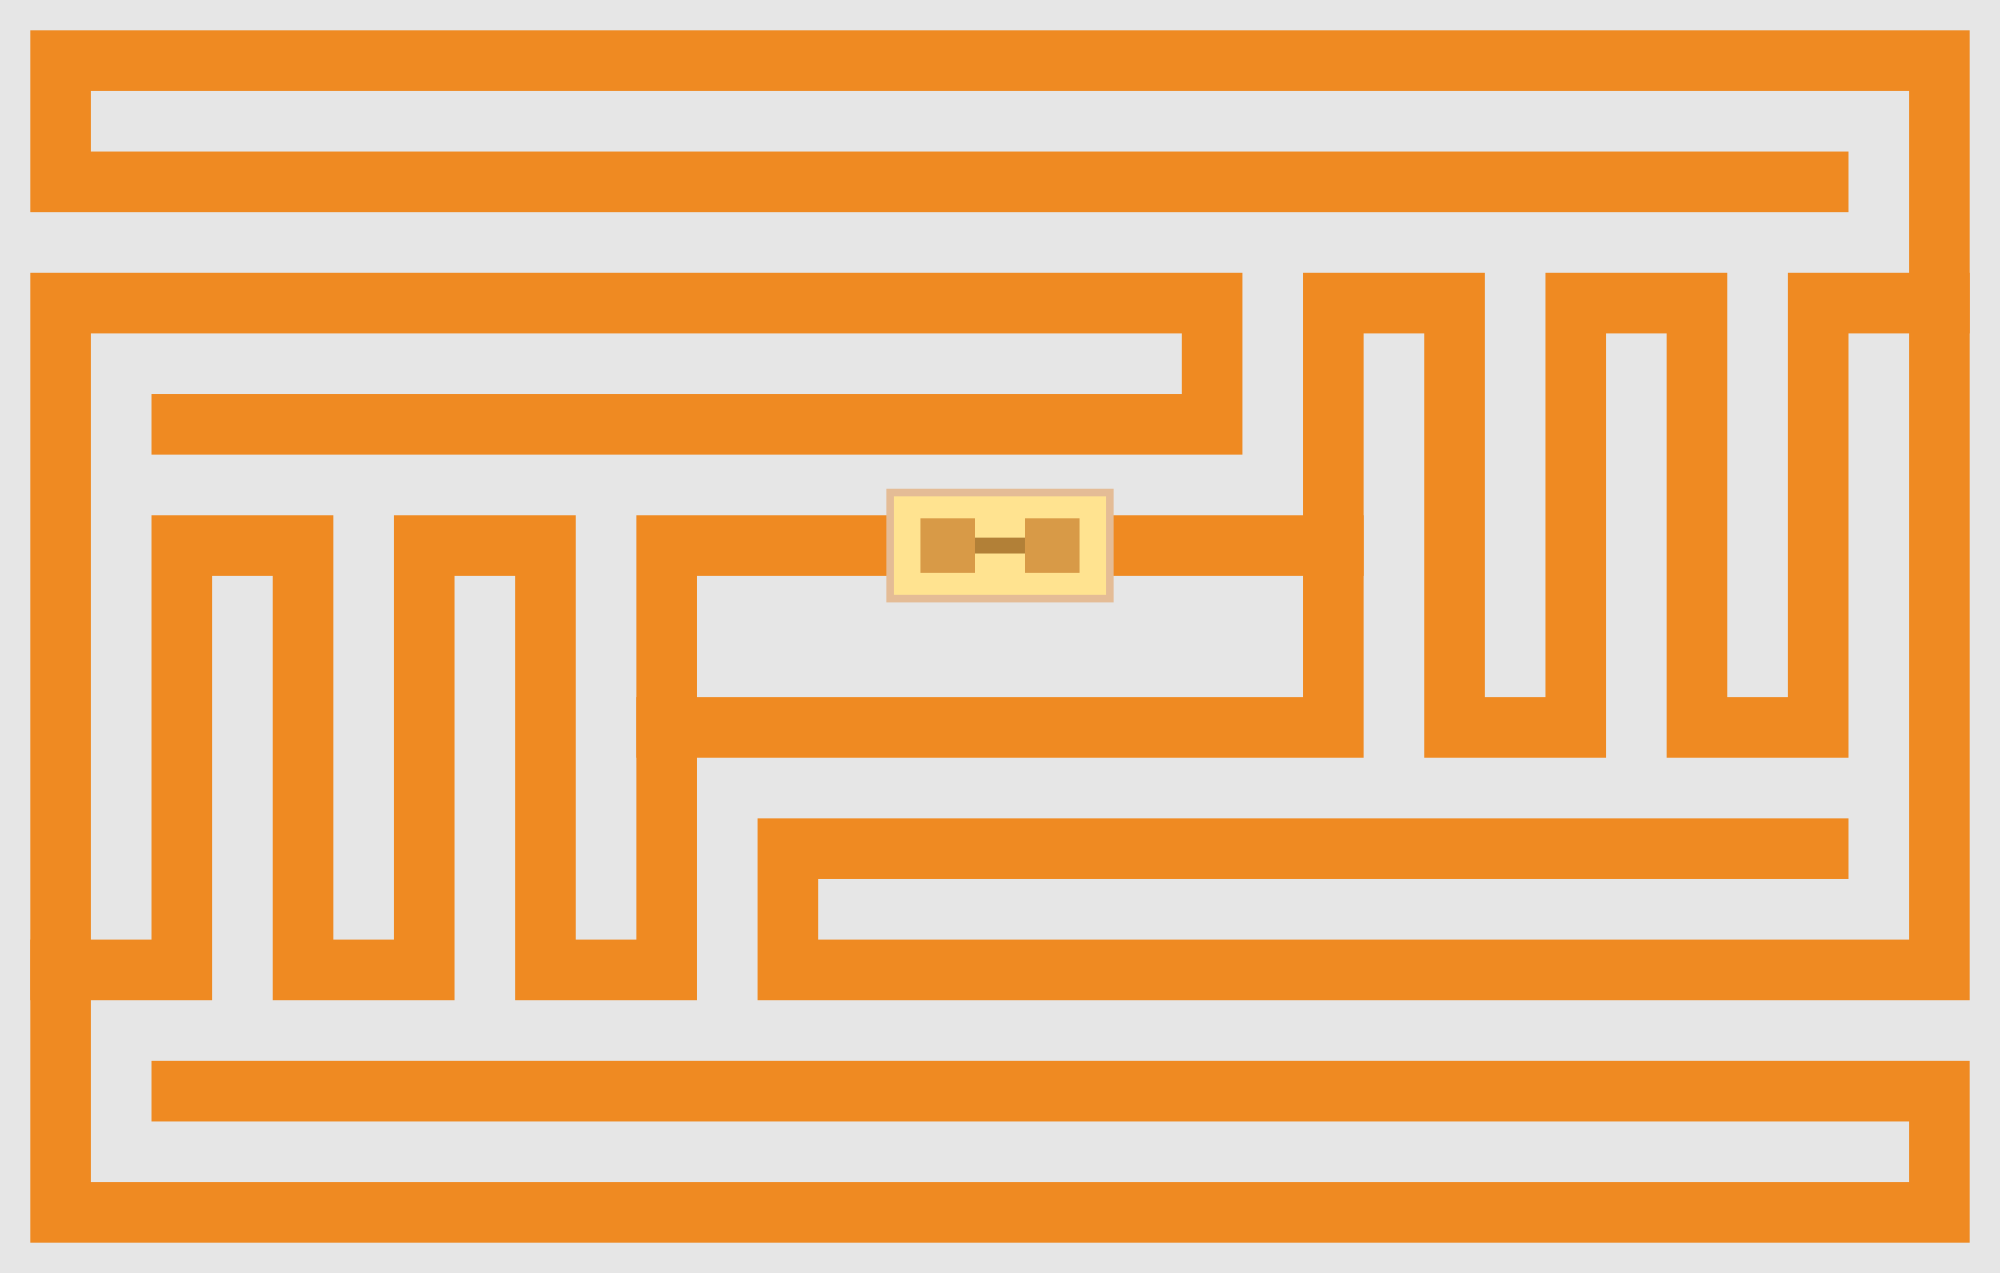
\includegraphics[width=0.4\textwidth]{images/rfid_tag.png}
    \caption{Παράδειγμα ολοκληρωμένου κυκλώματος ενός παθητικού RFID tag}
    \label{fig:rfid-tag}
\end{figure}

Αντίστοιχα, ένας RFID reader αποτελείται από μια κεραία, η οποία αναλαμβάνει την επικοινωνία με το RFID tag και μια μονάδα ελέγχου για την διαχείριση της ανταλλαγής δεδομένων με την εκάστοτε ετικέτα. Τα συστήματα RFID διακρίνονται σε ενεργητικά και παθητικά, ανάλογα με τον τρόπο επικοινωνίας της ετικέτας με τον αναγνώστη \cite{ElProCus_rfid, kaur2011rfid}. Στα ενεργητικά συστήματα οι ετικέτες τροφοδοτούνται αυτόνομα από μια εξωτερική πηγή τροφοδοσίας, όπως π.χ. μια μπαταρία, και έχουν την δυνατότητα να μεταδώσουν την πληροφορία τους σε μεγαλύτερες αποστάσεις. Αντίθετα, στα παθητικά συστήματα οι ετικέτες δεν έχουν δική τους πηγή τροφοδοσίας, αλλά λαμβάνουν την απαραίτητη ενέργεια από τους αναγνώστες RFID μέσω επαγωγικής σύζευξης κατά την φάση επικοινωνίας τους. Αν και τα παθητικά συστήματα έχουν πολύ μικρότερη εμβέλεια, αποτελούν την πλειοψηφία των RFID συστημάτων σήμερα και είναι αυτά που χρησιμοποιούνται σε εφαρμογές πλοήγησης για άτομα με μειωμένη όραση. Ένα τυπικό παράδειγμα λειτουργίας ενός τέτοιου συστήματος είναι η χρήση της πιστωτικής μας κάρτας κατά τη διάρκεια ανέπαφης συναλλαγής σε ένα κατάστημα. Η κάρτα μας παίζει τον ρόλο του RFID tag, ενώ η συσκευή POS του καταστήματος παίζει τον ρόλο του RFID reader. Μόλις η κάρτα βρεθεί αρκετά κοντά στο POS, λαμβάνει μέσω επαγωγικής σύζευξης την απαραίτητη ενέργεια από αυτό και τροφοδοτείται το ενσωματωμένο της ολοκληρωμένο κύκλωμα. Με αυτό τον τρόπο ενεργοποιείται ουσιαστικά η μετάδοση πληροφορίας, από την κάρτα προς το POS, η οποία πραγματοποιείται μέσω της κεραίας που υπάρχει και στα δύο μέρη.

\begin{figure}[H]
    \centering
    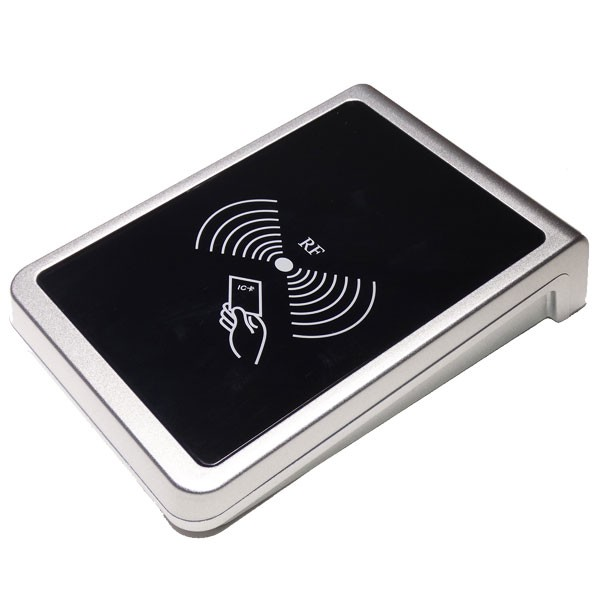
\includegraphics[width=0.4\textwidth]{images/rfid_reader.jpg}
    \caption{Παράδειγμα ενός RFID reader}
    \label{fig:rfid-reader}
\end{figure}

Η ενσωμάτωση των RFID συστημάτων σε συσκευές πλοήγησης για άτομα με προβλήματα όρασης αποτελεί μια έξυπνη λύση κυρίως σε εσωτερικούς χώρους, καθώς μπορούμε να τοποθετήσουμε πολλά RFID tags σε διαφορετικά σημεία-κόμβους μέσα στον χώρο, ή στο κτίριο που θέλουμε να καλύψουμε, ή ακόμα και κατά μήκος μιας διαδρομής που ακολουθούν τα άτομα με προβλήματα όρασης. Χρησιμοποιώντας έναν RFID reader τα άτομα αυτά θα είναι σε θέση να λαμβάνουν πληροφορίες σχετικά με την τοποθεσία στην οποία βρίσκονται και να καθοδηγούνται προς μια διαφορετική τοποθεσία, η οποία έχει ένα αντίστοιχο RFID tag.

Πραγματοποιώντας μια επισκόπηση της βιβλιογραφίας βρίσκουμε αρκετά συστήματα πλοήγησης που βασίζονται στην αξιοποίηση της τεχνολογίας RFID. Ένα αντιπροσωπευτικό παράδειγμα είναι αυτό που προτείνεται στο \cite{sammouda_mobile_2015}. Το προτεινόμενο σύστημα λειτουργεί σε εξωτερικούς και εσωτερικούς χώρους και αποτελείται από έναν RFID reader ενσωματωμένο στο λευκό μπαστούνι του χρήστη και πολλαπλά RFID tags διασκορπισμένα σε καίρια σημεία της διαδρομής του. Το σύστημα εντοπίζει την τοποθεσία του χρήστη είτε μέσω GPS, είτε μέσω ανάγνωσης του κοντινότερου RFID tag χρησιμοποιώντας τον ενσωματωμένο RFID reader. Σε περίπτωση που ο χρήστης θελήσει να κατευθυνθεί προς μια προκαθορισμένη τοποθεσία (π.χ. γραφείο, ή τουαλέτα) τότε το σύστημα τον προτρέπει να κινηθεί προς την σωστή κατεύθυνση, η οποία υπολογίζεται με χρήση ηλεκτρονικής πυξίδας, GPS και μέσω της ανάγνωσης του επόμενου RFID tag στο μονοπάτι του χρήστη. Πιο συγκεκριμένα, γίνεται σύγκριση της τωρινής θέσης του χρήστη σε σχέση με τον προορισμό και το κοντινότερο RFID tag και μέσω αυτής υπολογίζεται η κατάλληλη κατεύθυνση. Για να μπορεί λαμβάνει αξιόπιστες αποφάσεις το σύστημα διατηρεί μια βάση δεδομένων με όλες τις τοποθεσίες των τοποθετημένων RFID tags, συμπεριλαμβανομένων των αποστάσεων μεταξύ τους, οι οποίες ποικίλλουν από 4 έως 15 μέτρα.

\begin{figure}[H]
    \centering
    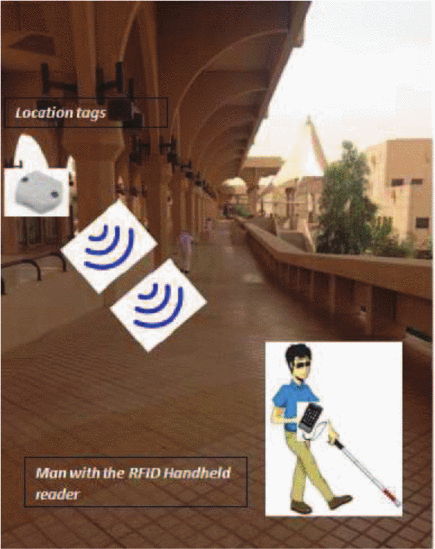
\includegraphics[width=0.6\textwidth]{images/rfid_paper.png}
    \caption{Περιγραφή του συστήματος που προτείνεται στο \cite{sammouda_mobile_2015}}
    \label{fig:sammouda_mobile}
\end{figure}
\hspace{1cm}

Παρατηρούμε ότι το παραπάνω σύστημα πετυχαίνει εν μέρει το σκοπό του, δηλαδή την καθοδήγηση του χρήστη προς ένα σημείο ενδιαφέροντος, αλλά γίνεται σαφές ότι ένα σύστημα πλοήγησης που βασίζεται σε RFID tags μπορεί να έχει ουσιαστικό νόημα μόνο σε εσωτερικούς χώρους ή σε συγκεκριμένες τοποθεσίες ενδιαφέροντος. Η ελεύθερη πλοήγηση του χρήστη μέσα σε μια πόλη δεν μπορεί να πραγματοποιηθεί, διότι σε αυτήν την περίπτωση θα απαιτούνταν ένας τεράστιος αριθμός από RFID tags κατά μήκος κάθε πιθανής διαδρομής του χρήστη!


\subsection{Learning-based}
Μια άλλη κατηγορία συστημάτων πλοήγησης είναι αυτή που βασίζεται στην αναγνώριση αντικειμένων/εμποδίων αξιοποιώντας τεχνικές της Μηχανικής Μάθησης (Machine Learning). Η βασική ιδέα πίσω από τέτοιου είδους συστήματα είναι ότι εκπαιδεύουμε έναν αλγόριθμο να αναγνωρίζει με πολύ μεγάλη ακρίβεια ένα αντικείμενο ή μια ομάδα αντικειμένων. Με άλλα λόγια, για να μπορέσει ο αλγόριθμος να εντοπίσει ένα συγκεκριμένο μοτίβο μέσα σε μια εικόνα, είτε αυτό είναι πρόσωπο, είτε είναι αντικείμενο, όπως π.χ. φανάρι, δρόμος κλπ, είναι απαραίτητο να έχει προηγηθεί μια διαδικασία "μάθησης", κατά την οποία παρέχουμε στον αλγόριθμο έναν πολύ μεγάλο αριθμό από γνωστές εικόνες που περιέχουν το μοτίβο που αναζητούμε. Ο αλγόριθμος λαμβάνει υπόψιν του όλες τις εικόνες που έχουν προηγηθεί και "δημιουργεί" ένα μοντέλο του αντικειμένου που θέλουμε να αναγνωρίζει. Αφού έχει επέλθει η διαδικασία της μάθησης το σύστημα είναι εκπαιδευμένο να αναγνωρίζει το συγκεκριμένο μοτίβο σε οποιαδήποτε άλλη νέα/άγνωστη εικόνα του δώσουμε ως είσοδο.

\begin{figure}[H]
    \centering
    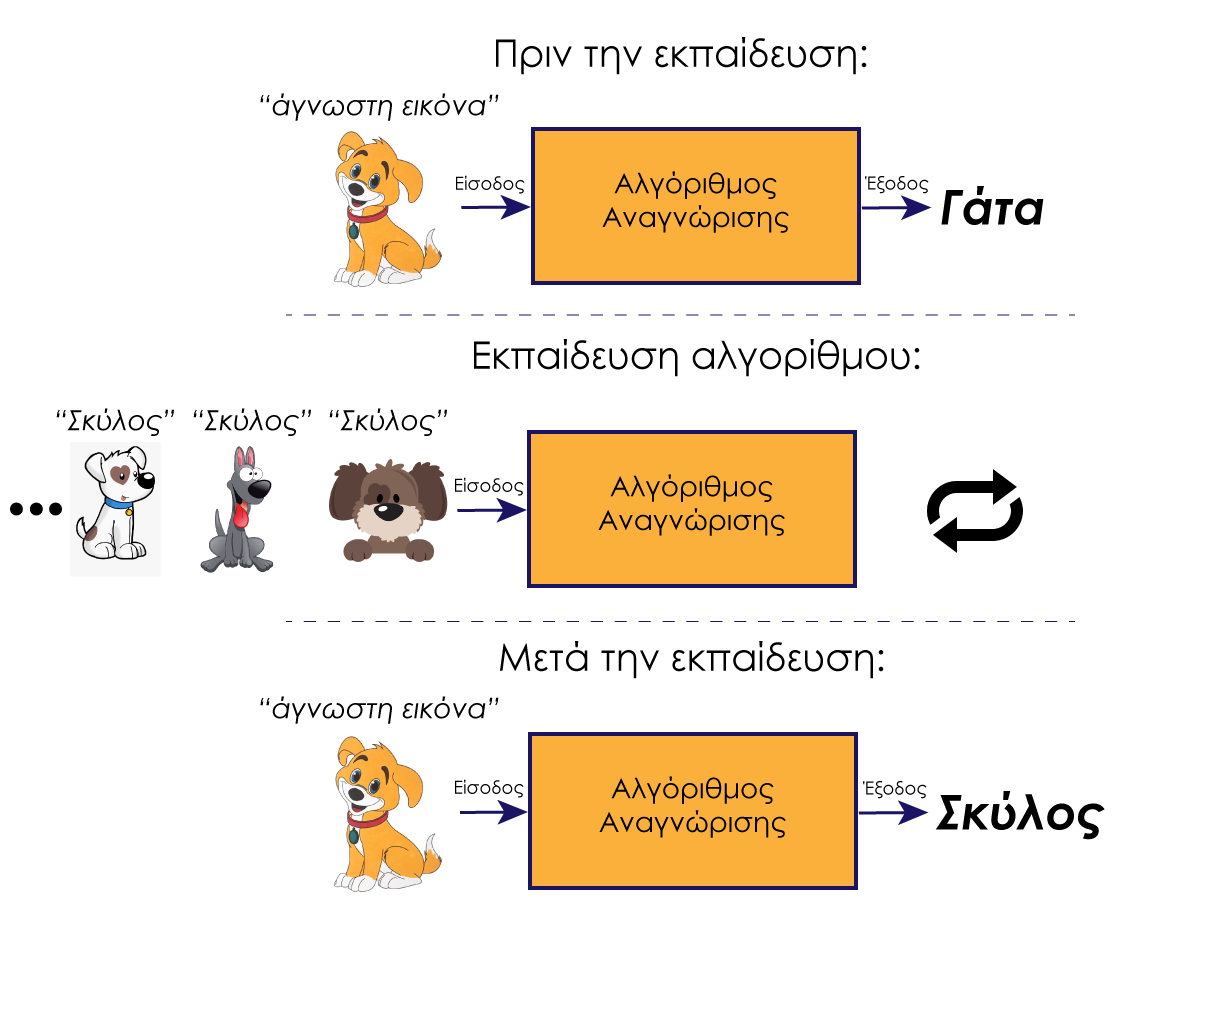
\includegraphics[width=0.8\textwidth]{images/learning_explained.png}
    \caption{Παράδειγμα εκπαίδευσης ενός αλγορίθμου μάθησης}
    \label{fig:learning-explained}
\end{figure}
\hspace{1cm}

Η εκπαίδευση αλγορίθμων για βελτιστοποιημένη αναγνώριση αντικειμένων δεν είναι μια νέα ιδέα στον τομέα της Υπολογιστικής Όρασης (Computer Vision), αλλά αποτελεί εξέλιξη της Αναγνώρισης Προτύπων (Pattern Recognition) η οποία μέχρι πρότινος χρησιμοποιούσε τις παραδοσιακές τεχνικές που σχετίζονται με την επεξεργασία εικόνας και σημάτων. Η ραγδαία αύξηση στην χρήση της μηχανικής μάθησης ως μέθοδο αναγνώρισης αντικειμένων συνέβη λόγω της αύξησης της διαθέσιμης επεξεργαστικής ισχύος τις τελευταίες δεκαετίες. Πλέον, ακόμα και ένα smartphone είναι ικανό να παρέχει επαρκή επεξεργαστική ισχύ για να εφαρμόσουμε μεθόδους μηχανικής μάθησης.

Οι εργασίες μηχανικής μάθησης χωρίζονται σε 3 (τρεις) μεγάλες κατηγορίες \cite{russell2016artificial} :

\begin{itemize}
    \item \textbf{Supervised Learning} (Επιβλεπόμενη Μάθηση): Ο αλγόριθμος μάθησης κατασκευάζει μια συνάρτηση που απεικονίζει τα δεδομένα εισόδου (σύνολο εκπαίδευσης) σε γνωστές επιθυμητές εξόδους. Η μάθηση χαρακτηρίζεται επιβλεπόμενη επειδή υπάρχει κάποιος "επιβλέπων" που παρέχει την σωστή τιμή εξόδου της συνάρτησης για το σύνολο εκπαίδευσης. Στόχος του αλγορίθμου είναι να "γενικεύσει" αυτήν την συνάρτηση, ώστε να μπορεί να προγνώσει με ακρίβεια την έξοδο του συστήματος σε δεδομένα εισόδου με αρχικά άγνωστη έξοδο. Μερικά παραδείγματα τεχνικών supervised learning είναι:
    \begin{itemize}
        \item Δέντρα Απόφασης (Decision Trees)
        \item Μάθηση Κανόνων (Rule Learning)
        \item Μάθηση κατά Περίπτωση (Instance Based Learning)
        \item Μάθηση κατά Bayes
        \item Γραμμική Παρεμβολή (Linear Regression)
        \item Νευρωνικά Δίκτυα (Neural Networks)
        \item Μηχανές Διανυσμάτων Υποστήριξης (Support Vector Machines)
    \end{itemize}
    
    \item \textbf{Unsupervised Learning} (Μη Επιβλεπόμενη Μάθηση):
    Ο αλγόριθμος αναλύει το σύνολο των δεδομένων εισόδου και κατασκευάζει ένα μοντέλο υπό μορφή συσχετίσεων ή ομαδοποιήσεων, χωρίς να γνωρίζει τις επιθυμητές εξόδους. Σαν αποτέλεσμα (έξοδος) προκύπτουν πρότυπα (περιγραφές), κάθε ένα από τα οποία περιγράφει ένα μέρος από τα δεδομένα. Τέτοιου τύπου αλγόριθμοι χρησιμοποιούνται κυρίως σε προβλήματα:
    \begin{itemize}
        \item Ανάλυσης Συσχετισμών (Association Analysis)
        \item Ομαδοποίησης (Clustering)
    \end{itemize}
    
    \item \textbf{Reinforcement Learning} (Ενισχυτική Μάθηση):
    Αποτελεί την πιο "αυτόνομη" μορφή αλγορίθμων μάθησης, όπου το σύστημα αλληλεπιδρά άμεσα με το περιβάλλον και μαθαίνει μια στρατηγική ενεργειών, που αποσκοπεί στην επίτευξη ενός στόχου, π.χ. οδήγηση ενός οχήματος. Χρησιμοποιείται κυρίως σε προβλήματα Σχεδιασμού (Planning), όπως για παράδειγμα ο έλεγχος κίνησης ρομπότ και η βελτιστοποίηση εργασιών σε εργοστασιακούς χώρους.
\end{itemize}

Στα συστήματα πλοήγησης χρησιμοποιείται κυρίως το supervised learning και πιο συγκεκριμένα εκπαιδεύονται Νευρωνικά Δίκτυα για την αναγνώριση του περιβάλλοντος.

\subsubsection{Νευρωνικά δίκτυα}
Ένα τεχνητό νευρωνικό δίκτυο - ΤΝΔ (Artificial Neural Network - ANN) στην μηχανική μάθηση είναι ένας αλγόριθμος εκμάθησης που εμπνέεται από τη δομή και τις λειτουργικές πτυχές των βιολογικών νευρωνικών δικτύων του ανθρώπινου εγκεφάλου. Με άλλα λόγια ο όρος "Νευρωνικά Δίκτυα" περιγράφει έναν αριθμό από διαφορετικά μαθηματικά μοντέλα που προσπαθούν να μιμηθούν τη συμπεριφορά των βιολογικών νευρώνων. Όπως τα νευρωνικά δίκτυα του εγκεφάλου περιέχουν έναν πολύ μεγάλο αριθμό από μεμονωμένα διακριτά στοιχεία, τους νευρώνες, έτσι και τα τεχνητά νευρωνικά δίκτυα αποτελούνται από έναν μεγάλο αριθμό απλών κόμβων (nodes) διασυνδεδεμένων μεταξύ τους, που παίζουν τον ρόλο των νευρώνων και οι οποίοι οργανώνονται σε στρώματα (layers). 
\begin{figure}[H]
    \centering
    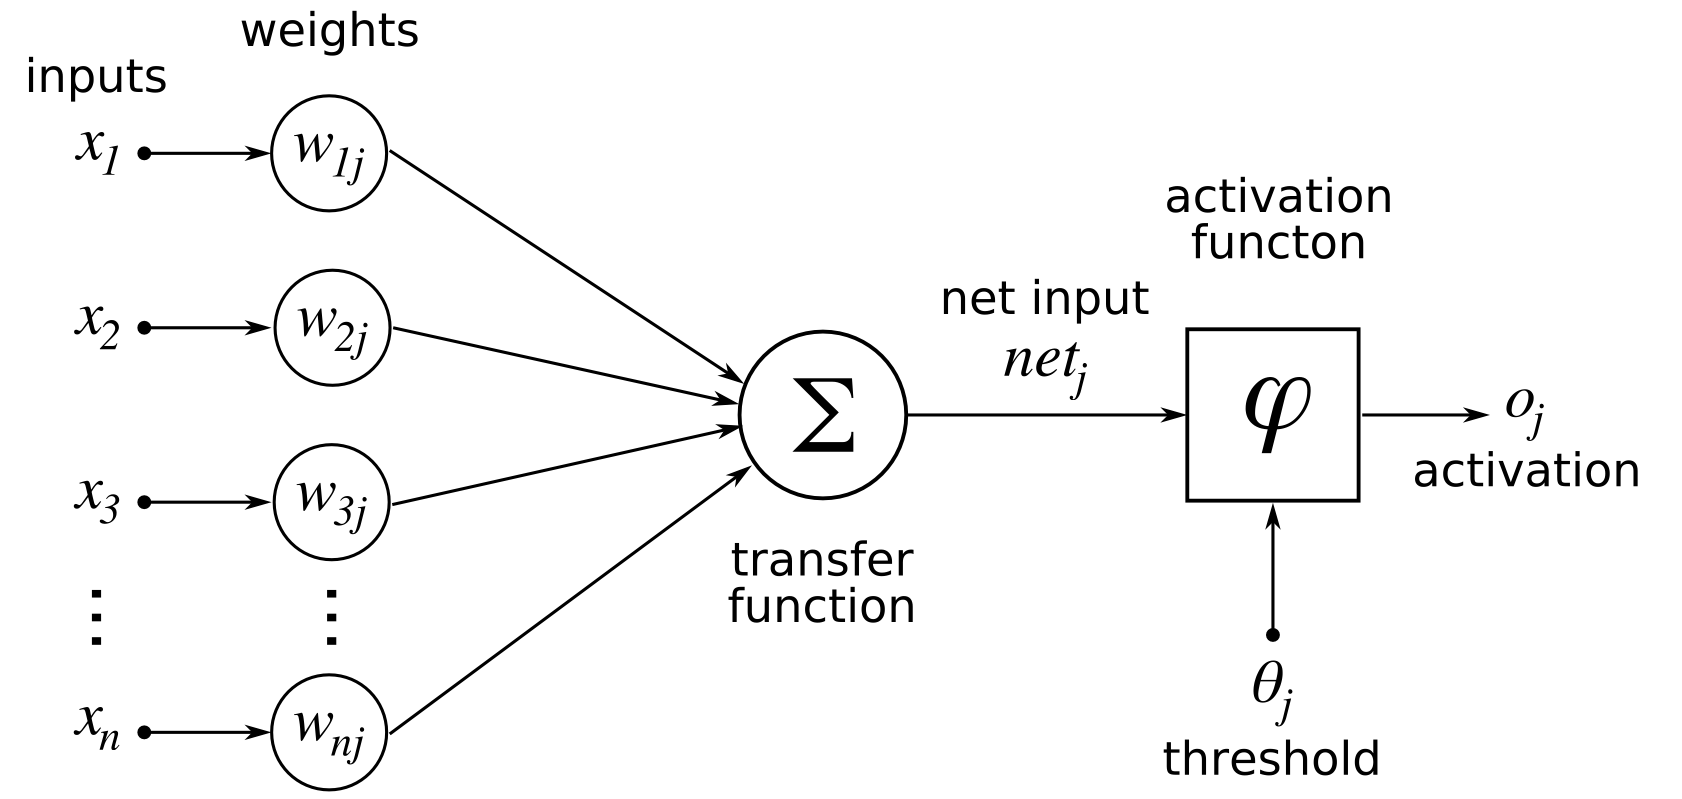
\includegraphics[width=0.6\textwidth]{images/art_neuron.png}
    \caption{Απεικόνιση λειτουργίας του απλούστερου τεχνητού νευρωνικού δικτύου, που ονομάζεται \textit{Perceptron} και αποτελείται από έναν μόνο νευρώνα}
    \label{fig:art-neuron}
\end{figure}
% \footnotetext{Chrislb (\url{https://commons.wikimedia.org/wiki/File:ArtificialNeuronModel\textunderscore english.png}), "ArtificialNeuronModel english", \url{https://creativecommons.org/licenses/by-sa/3.0/legalcode}}
\hspace{1cm}
Κάθε τεχνητός νευρώνας αποτελείται από πολλές εισόδους $x_i$ και μία μόνο έξοδο $y$. Κάθε είσοδος $x_i$ πολλαπλασιάζεται με ένα βάρος $w_i$ και αθροίζεται μέσω της συνάρτησης αθροίσματος (summation function) F, ως εξής: \[F = \sum_{i}^{n} x_i w_i\] Ο τεχνητός νευρώνας δίνει έξοδο μέσω της συνάρτησης ενεργοποίησης (activation function), μόνο όταν το σταθμισμένο άθροισμα $F$ είναι μεγαλύτερο μιας ορισμένης τιμής κατωφλίου (threshold value) $\theta$ \cite{Grossi2008}, δηλαδή όταν, \[\sum_{i}^{n} x_i w_i - \theta > 0\]

Το απλούστερο νευρωνικό δίκτυο Perceptron \cite{rosenblatt1961principles} (σχήμα \ref{fig:art-neuron}) αποτελείται από έναν μόνο νευρώνα και ένα επίπεδο. Συνήθως τα ΤΝΔ είναι πιο σύνθετα και οργανώνονται σε πολλαπλά επίπεδα (layers) τα οποία καλούνται και στρώματα. Τα ενδιάμεσα επίπεδα ονομάζονται κρυμμένα επίπεδα (hidden layers) και δεν είναι απαραίτητο να υπάρχουν. Οι κόμβοι-νευρώνες που υπάρχουν σε κάθε επίπεδο είναι συνδεδεμένοι μεταξύ τους, ώστε κάθε κόμβος-νευρώνας να έχει συνδέσμους με πολλούς άλλους κόμβους του ίδιου ή άλλου επιπέδου. Το δίκτυο δέχεται τις εισόδους $x_i$ στο επίπεδο εισόδου (input layer), το οποίο αλληλεπιδρά με τα κρυμμένα ενδιάμεσα επίπεδα, και παρέχει την έξοδό του μέσω του επιπέδου εξόδου (output layer).

\begin{figure}[H]
    \centering
    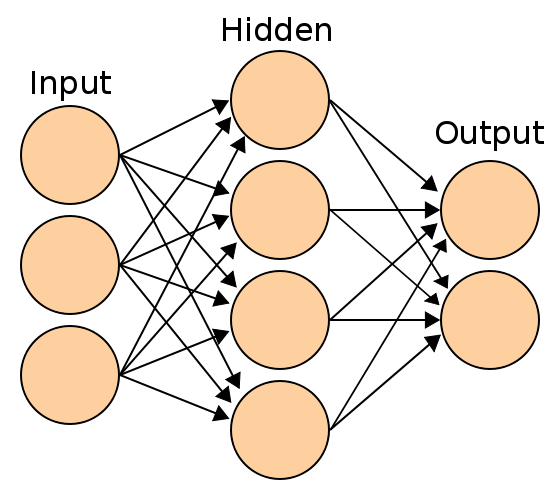
\includegraphics[width=0.4\textwidth]{images/ann_layers.png}
    \caption{Δομή επιπέδων σε ένα απλό τεχνητό νευρωνικό δίκτυο με ένα ενδιάμεσο κρυμμένο επίπεδο}
    \label{fig:ann-layers}
\end{figure}
% \footnotetext{en:User:Cburnett (\url{https://commons.wikimedia.org/wiki/File:Artificial\textunderscore neural\textunderscore network.svg}), "ArtificialNeuronModel english", \url{https://creativecommons.org/licenses/by-sa/3.0/legalcode}}

Σκοπός της παρούσας διπλωματικής εργασίας δεν είναι η αναλυτική περιγραφή των νευρωνικών δικτύων, γι'αυτό θα προχωρήσουμε κατευθείαν στην εφαρμογή τους όσον αφορά τα συστήματα πλοήγησης για άτομα με προβλήματα όρασης.

Η σημασία των νευρωνικών δικτύων στα συστήματα πλοήγησης σχετίζεται με την ακρίβεια που πετυχαίνουν στην αναγνώρισή αντικειμένων. Πιο συγκεκριμένα, τα τελευταία χρόνια χρησιμοποιούνται τα λεγόμενα Deep Neural Networks (Βαθιά Νευρωνικά Δίκτυα), τα οποία αποτελούνται από πολλά κρυμμένα επίπεδα και παρέχουν πολύ υψηλή ακρίβεια σε εφαρμογές όπως η αναγνώριση προσώπων, η κατηγοριοποίηση αντικειμένων κλπ. Ένα χαρακτηριστικό παράδειγμα αποτελεί το σύστημα που προτείνεται στο \cite{lin2017simple}, το οποίο χρησιμοποιεί την κάμερα από το smartphone του χρήστη και έναν υπολογιστή ως server. Το κύριο χαρακτηριστικό της συγκεκριμένης έρευνας είναι ότι, καθώς ο χρήστης πλοηγείται στον χώρο, το smartphone τραβάει φωτογραφίες από τον χώρο μπροστά από τον χρήστη και τις στέλνει, μέσω διαδικτύου, στον server όπου γίνεται η επεξεργασία τους. Πιο συγκεκριμένα, πριν την αποστολή της φωτογραφίας, γίνεται επιλογή των χαρακτηριστικών (feature selection) που θα χρησιμοποιηθούν ως είσοδοι στο νευρωνικό δίκτυο στην πλευρά του server. Ο server "τρέχει" δύο διαφορετικούς αλγορίθμους ταξινόμησης εικόνων, ανάλογα την ταχύτητα της διαδικτυακής σύνδεσης του χρήστη. Όταν η ταχύτητα σύνδεσης είναι υψηλή εφαρμόζεται ο αλγόριθμος Faster R-CNN (Faster Region-based Convolutional Neural Network), ενώ όταν η ταχύτητα σύνδεσης είναι αργή εφαρμόζεται ο αλγόριθμος YOLO (You Only Look Once). Αφού ο κάθε αλγόριθμος έχει εκπαιδευτεί να αναγνωρίζει και να ταξινομεί μια ομάδα αντικειμένων, το σύστημα αποστέλλει τα features, που έχουν εξαχθεί κατά τη διαδικασία του feature selection, στον server και αυτός με την σειρά του ταξινομεί την δοθείσα φωτογραφία. 

Όπως αναφέρεται και στην ίδια την έρευνα, αν και η χρήση των νευρωνικών δικτύων έχει ως αποτέλεσμα αρκετά υψηλή ακρίβεια, απαιτείται ιδιαίτερα υψηλή επεξεργαστική ισχύς, κάτι που δικαιολογεί και την χρήση του server ως εξωτερική μονάδα επεξεργασίας. Η χρήση του server και η αναγκαία μετάδοση των εικόνων από το smartphone προς αυτόν, συνεπάγεται την ύπαρξη μιας μικρής καθυστέρησης, η οποία μπορεί να γίνει σημαντικά μεγαλύτερη ανάλογα την ταχύτητα μετάδοσης και την πολυπλοκότητα του δικτύου που χρησιμοποιείται, έως ότου το σύστημα αποφανθεί για τον τύπο του εμποδίου που βρίσκεται μπροστά από τον χρήστη. Με άλλα λόγια, η έλλειψη επεξεργαστικής ισχύος οδηγεί σε προβλήματα όσον αφορά την real-time αναγνώριση αντικειμένων.

Καταλήγοντας, είναι αναγκαίο να τονίσουμε το γεγονός ότι τα βαθιά νευρωνικά δίκτυα αποτελούν πλέον μια πολύ αξιόπιστη λύση όσον αφορά τον εντοπισμό και την αναγνώριση εμποδίων σε συστήματα πλοήγησης, καθώς παρέχουν μεγάλα ποσοστά ακρίβειας και είναι σε θέση να αναγνωρίζουν ταυτόχρονα πολλαπλά αντικείμενα σε μια φωτογραφία. Από την άλλη πλευρά, όμως, ο περιοριστικός παράγοντας των υψηλών απαιτήσεων σε επεξεργαστική ισχύ και η αναγκαιότητα εκπαίδευσης των νευρωνικών δικτύων εκ των προτέρων, αποτελούν τροχοπέδη στην πλήρη αξιοποίησή τους και εφαρμογή τους σε φορητά συστήματα πλοήγησης για άτομα με μειωμένη όραση. Αξίζει, δε, να τονίσουμε ότι η εκπαίδευση των νευρωνικών δικτύων προϋποθέτει την ύπαρξη κατάλληλου σετ δεδομένων (dataset), για κάθε ξεχωριστό μοτίβο/αντικείμενο που θέλουμε να αναγνωρίζει το σύστημα, τα οποία δεν είναι πάντα διαθέσιμα. Αυτός είναι και ο λόγος που η παρούσα διπλωματική εργασία χρησιμοποιεί παραδοσιακές μεθόδους αναγνώρισης αντικειμένων, όπως αυτές που περιγράφονται παρακάτω.

\subsection{Vision-based}
Η κατηγορία αυτή των συστημάτων περιλαμβάνει τα συστήματα εκείνα που βασίζονται σε παραδοσιακές μεθόδους ανίχνευσης εμποδίων και αναγνώρισης αντικειμένων. Πιο συγκεκριμένα, η πλειοψηφία των συστημάτων πλοήγησης χρησιμοποιεί διάφορους αισθητήρες απόστασης, όπως αισθητήρες υπερήχων, LiDaR κλπ, για την ανίχνευση της ύπαρξης εμποδίου μπροστά από τον χρήστη. Παράλληλα, η ανίχνευση και η αναγνώριση του είδους των αντικειμένων γίνεται με μεθόδους ψηφιακής επεξεργασίας εικόνας. Παρακάτω αναλύεται η λειτουργία των βασικών αισθητήρων που εντοπίζονται σε ένα τέτοιο σύστημα.

\subsubsection{Ultrasonic sensors}
Η χρήση υπερήχων ανέκαθεν αποτελούσε μια από τις πιο γνωστές μεθόδους μέτρησης μικρών αποστάσεων και ανίχνευσης αντικειμένων, ενώ ακόμη και σήμερα αξιοποιούνται σε πολλές εφαρμογές, όπως είναι ο μη καταστροφικός έλεγχος (non destructive inspection) στη βιομηχανία ή η εξέταση υπερήχων στην απεικονιστική ιατρική. Ο άνθρωπος μπορεί να ακούσει ήχους σε ένα εύρος συχνοτήτων από 20 Hz έως 20 KHz (Σχήμα \ref{fig:ultrasound-range}). Οι υπέρηχοι είναι ηχητικά κύματα που έχουν συχνότητες μεγαλύτερες από 20 KHz, άρα δεν γίνονται αντιληπτοί από έναν φυσιολογικό άνθρωπο. Η σημασία των υπερήχων στην πλοήγηση και τον ηχο-εντοπισμό (echolocation) ανακαλύφθηκε για πρώτη φορά από τον Ιταλό Lazzaro Spallanzan, ο οποίος μελέτησε την συμπεριφορά των νυχτερίδων και παρατήρησε ότι προσανατολίζονται χρησιμοποιώντας υπερήχους και όχι όραση \cite{spallanzani1794lettere}. 

\begin{figure}[H]
    \centering
    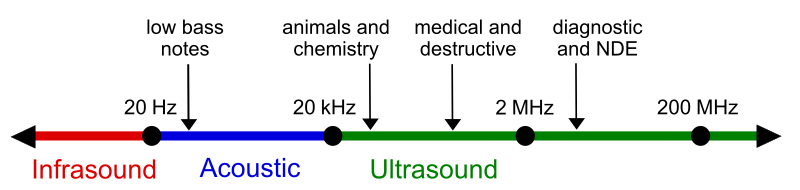
\includegraphics[width=0.6\textwidth]{images/Ultrasound_range_diagram.png}
    \caption{Διάγραμμα εύρους ηχητικών συχνοτήτων}
    \label{fig:ultrasound-range}
\end{figure}
\hspace{1cm}
% Ultrasound_range_diagram.png: The original uploader was LightYear at English Wikipedia. Ultrasound_range_diagram_png_(sk).svg: The original uploader was LightYear at English Wikipedia. derivative work: Coolth (talk) (https://commons.wikimedia.org/wiki/File:Ultrasound_range_diagram.svg), „Ultrasound range diagram“, https://creativecommons.org/licenses/by-sa/3.0/legalcode

Οι αισθητήρες υπερήχων αποτελούνται από έναν πομπό και έναν δέκτη υπερήχων και εκτιμούν την απόσταση ενός στόχου λαμβάνοντας υπόψη τους την αντανάκλαση ενός ραδιοκύματος ή ενός ηχητικού σήματος πάνω στο στόχο (Σχήμα \ref{fig:sonar-principle}). Για να το επιτύχουν αυτό χρησιμοποιούν τον χρόνο που έκανε το σήμα για να καλύψει την απόσταση από τον αισθητήρα στο αντικείμενο και πίσω. Η απόσταση ενός αντικειμένου μπροστά από τον αισθητήρα υπερήχου δίνεται ως εξής \cite{Theworki10:online}: \[distance = \frac{Time\textunderscore of\textunderscore Flight \times Speed\textunderscore of\textunderscore Sound}{2}\]

\begin{figure}[H]
    \centering
    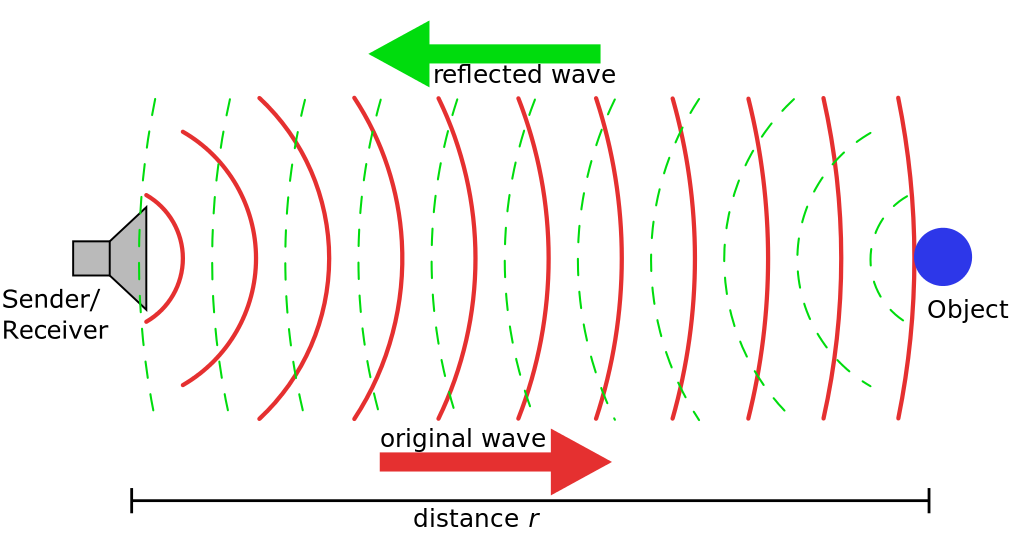
\includegraphics[width=0.6\textwidth]{images/Sonar_Principle.png}
    \caption{Αρχή λειτουργίας αισθητήρα υπερήχων}
    \label{fig:sonar-principle}
\end{figure}
\hspace{1cm}
% Georg Wiora (Dr. Schorsch) (https://commons.wikimedia.org/wiki/File:Sonar_Principle_EN.svg), „Sonar Principle EN“, https://creativecommons.org/licenses/by-sa/3.0/legalcode

Χάρη στην ευκολία χρήσης τους και το χαμηλό τους κόστος, πολλές εφαρμογές πλοήγησης αξιοποιούν τους αισθητήρες υπερήχων για να εντοπίζουν εμπόδια κατά μήκος του μονοπατιού του χρήστη. Ένα αντιπροσωπευτικό παράδειγμα αποτελεί η σχετική υλοποίηση στο \cite{bousbia2007ultrasonic}, όπου το προτεινόμενο σύστημα χρησιμοποιεί αποκλειστικά αισθητήρες υπερήχων για την καθοδήγηση του χρήστη. Χρησιμοποιώντας δύο αισθητήρες οι οποίοι εκπέμπουν παλμούς υπερήχων στα 40 KHz, είναι σε θέση να εντοπίζει συμπαγή αντικείμενα σε απόσταση 0.03 έως 6 μέτρα, και ανάλογα την εκτίμηση της απόστασης ειδοποιεί τον χρήστη μέσω δονήσεων.

\begin{figure}[H]
    \centering
    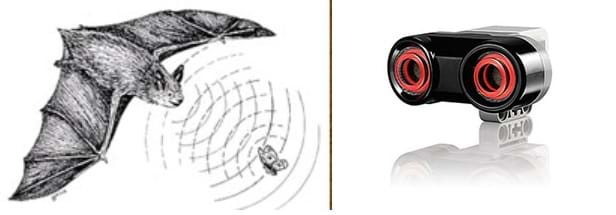
\includegraphics[width=0.6\textwidth]{images/ultrasonic_example.jpg}
    \caption{Αριστερά: Απεικόνιση του ηχο-εντοπισμού της νυχτερίδας. Δεξιά: Παράδειγμα ενός τυπικού αισθητήρα υπερήχων με έναν δέκτη και έναν πομπό.}
    \label{fig:sonar-example}
\end{figure}
\hspace{1cm}
% https://www.teachengineering.org/lessons/view/umo_sensorswork_lesson06
Αν και η χρήση υπερήχων λειτουργεί ικανοποιητικά σε εσωτερικούς χώρους, η αξιοποίησή τους σε εξωτερικά περιβάλλοντα έχει αρκετά μειονεκτήματα, κυρίως, λόγω της παρεμβολής από άλλα ηχητικά σήματα του ίδιου φάσματος. Επίσης, ένα μεγάλο μειονέκτημα αυτής της μεθόδου είναι η αδυναμία αναγνώρισης του είδους του αντικειμένου που ανιχνεύεται.

\subsubsection{LiDAR sensors}
Οι αισθητήρες Light Detection And Ranging, εν συντομία LiDAR, είναι συσκευές που λειτουργούν αξιοποιώντας το φως και την αντανάκλασή του πάνω σε επιφάνειες. Η αρχή λειτουργίας τους μοιάζει πολύ με εκείνη των αισθητήρων υπερήχων, μόνο που στην περίπτωση αυτή δεν εκπέμπουν υπερήχους, αλλά βασίζονται στην εκπομπή παλμικής ακτινοβολίας λέιζερ στην ατμόσφαιρα. Οι ακτίνες αντανακλούν πάνω στα αντικείμενα του περιβάλλοντος και ο αισθητήρας καταγράφει την ανακλώμενη ακτινοβολία λέιζερ, υπολογίζοντας την απόσταση των αντικειμένων ως εξής \cite{wwwlidar41:online}: \[distance = \frac{Time\textunderscore of\textunderscore Flight \times Speed\textunderscore of\textunderscore Light}{2}\]

Πιο συγκεκριμένα, οι αισθητήρες LiDAR εκπέμπουν ακτίνες φωτός στο υπεριώδες, στο ορατό, ή κοντά στο υπέρυθρο φάσμα ηλεκτρομαγνητικής ακτινοβολίας και είναι πολύ πιο ακριβείς από τους αντίστοιχους αισθητήρες υπερήχων, ενώ μπορούν επίσης να χρησιμοποιηθούν σε ένα μεγάλο εύρος υλικών, συμπεριλαμβανομένου μη-μεταλλικών αντικειμένων, βράχων, βροχής, ακόμα και σε μοριακό επίπεδο. Αυτή η μεγάλη ευελιξία των αισθητήρων LiDAR τους καθιστά πολύ χρήσιμους για την κατασκευή 3D αναπαραστάσεων των αντικειμένων-στόχων (3D reconstruction). Οι εφαρμογές τους περιλαμβάνουν την χρήση τους σε αεροφωτογραφίες, σε αυτόνομα οχήματα κ.α., ενώ αξίζει να τονίσουμε το γεγονός πως λειτουργούν καλύτερα σε εσωτερικά περιβάλλοντα, εξαιτίας την επίδρασης της υπέρυθρης ακτινοβολίας του ήλιου σε εξωτερικούς χώρους \cite{wiki:lidar}.

\begin{figure}[H]
    \centering
    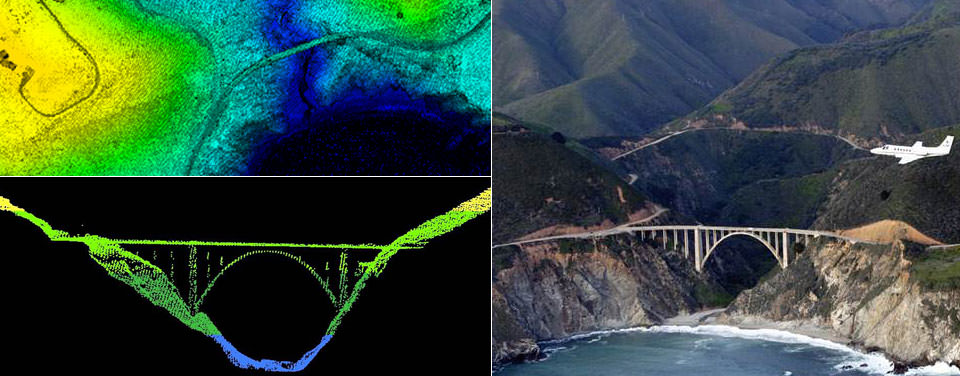
\includegraphics[width=0.8\textwidth]{images/lidar_3d_map.jpg}
    \caption{3D ψηφιακή αναπαράσταση μιας τοποθεσίας μέσω LiDAR}
    \label{fig:lidar-3dmap}
\end{figure}
\hspace{1cm}
% https://oceanservice.noaa.gov/facts/lidar.html
\begin{figure}[H]
    \centering
    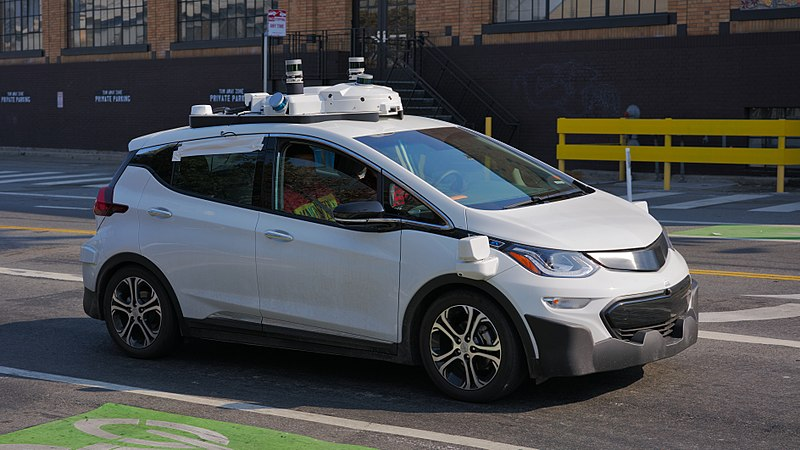
\includegraphics[width=0.6\textwidth]{images/lidar_car.jpg}
    \caption{Αισθητήρες LiDAR τοποθετούνται πάνω σε αυτόνομα οχήματα}
    \label{fig:lidar-car}
\end{figure}
\hspace{1cm}
% Dllu (https://commons.wikimedia.org/wiki/File:Cruise_Automation_Bolt_EV_third_generation_in_San_Francisco.jpg), https://creativecommons.org/licenses/by-sa/4.0/legalcode
Αν και η χρήση LiDAR δεν είναι τόσο διαδεδομένη σε φορητά συστήματα πλοήγησης, κυρίως, λόγω του όγκου τους και του υψηλού κόστους, υπάρχουν προσπάθειες που αναδεικνύουν την χρησιμότητά τους. Για παράδειγμα, στο \cite{miles2016lidar} προτείνεται ένα σύστημα πλοήγησης για άτομα με προβλήματα όρασης που βασίζεται αποκλειστικά στη χρήση ενός 2D LiDAR αισθητήρα (Σχήμα \ref{fig:lidar-example}), ο οποίος σκανάρει το περιβάλλον γύρω του σε ένα εύρος 270\degree και στέλνει τα δεδομένα σε μια μονάδα ψηφιακής επεξεργασίας σημάτων. Το αποτέλεσμα ανακοινώνεται στον χρήστη μέσω ηχητικών ειδοποιήσεων.
\begin{figure}[H]
    \centering
    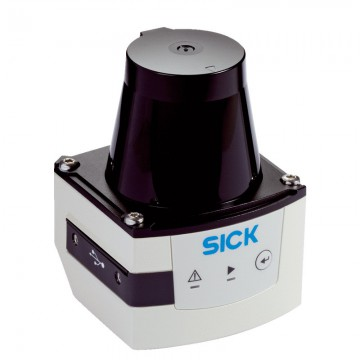
\includegraphics[width=0.4\textwidth]{images/lidar_example.jpg}
    \caption{Ο αισθητήρας LiDAR που χρησιμοποιείται στο \cite{miles2016lidar}}
    \label{fig:lidar-example}
\end{figure}
\hspace{1cm}

\subsubsection{RGB-D Camera}
Η πλειοψηφία των συστημάτων πλοήγησης για άτομα με προβλήματα όρασης χρησιμοποιεί κάμερες με ενσωματωμένο αισθητήρα βάθους, οι λεγόμενες RGB-D κάμερες. Τέτοια συστήματα είναι σε θέση τόσο να ανιχνεύουν τα εμπόδια μπροστά από τον χρήστη μέσω του αισθητήρα βάθους, όσο και να αναγνωρίζουν τον τύπο του εμποδίου, ή του αντικειμένου που μας ενδιαφέρει, μέσω της επεξεργασίας της RGB εικόνας που λαμβάνεται από την κάμερα.

Η πιο διαδεδομένη κάμερα με ενσωματωμένο αισθητήρα βάθους είναι η \textit{Microsoft Kinect RGB-D Camera}, η οποία πέρα από την αρχική της χρήση για το XBOX 360, αποτελεί την λύση σε πολλές πειραματικές προσπάθειες για ανάπτυξη φορητών συστημάτων πλοήγησης.
\begin{figure}[H]
    \centering
    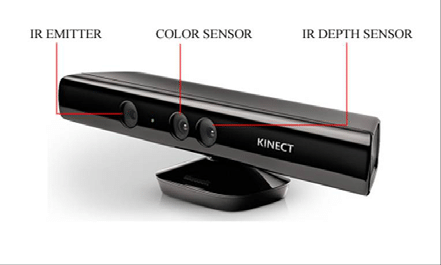
\includegraphics[width=0.6\textwidth]{images/kinect2.png}
    \caption{Ο αισθητήρας Kinect}
    \label{fig:kinect}
\end{figure}
\hspace{1cm}

Αυτοί οι αισθητήρες αποτελούνται συνήθως από έναν πομποδέκτη υπέρυθρης ακτινοβολίας (Infrared - IR) και έναν αισθητήρα RGB. Η αρχή λειτουργίας τους είναι η εξής: ο πομπός υπερύθρων προβάλλει στον χώρο ένα μοτίβο από σημεία υπέρυθρου φωτός (Structured Light technique) και ο δέκτης δέχεται τις ανακλώμενες ακτίνες. Το μοτίβο σημείων που εκπέμπεται παραμορφώνεται ανάλογα την επιφάνεια και τα αντικείμενα στα οποία ανακλάται. Στη συνέχεια γίνεται μια σύγκριση της αρχικής δομής των σημείων φωτός και αυτής που λήφθηκε από τον δέκτη. Έτσι, ανάλογα την παραμόρφωση που έχει υποστεί η δομή αυτή, παράγεται μια εικόνα βάθους, στην οποία κάθε pixel αντικατοπτρίζει την καρτεσιανή απόσταση (σε χιλιοστά) από την επιφάνεια της κάμερας μέχρι το κοντινότερο αντικείμενο στις συγκεκριμένες $x$,$y$ συντεταγμένες \cite{wiki:kinect}.
\begin{figure}[H]
    \centering
    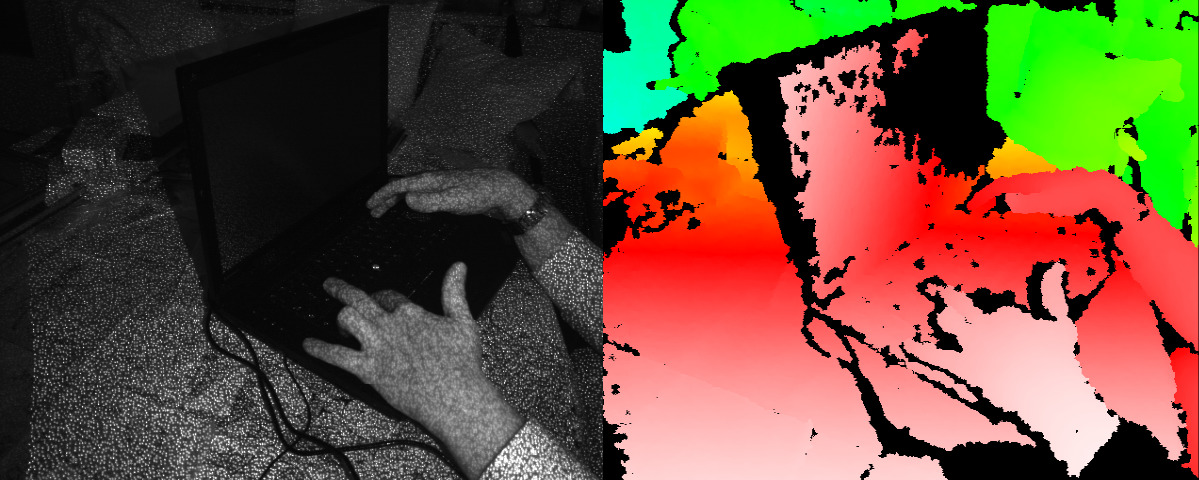
\includegraphics[width=\textwidth]{images/ir_structured_light.jpg}
    \caption{Αριστερά: Το μοτίβο από σημεία υπέρυθρου φωτός που εκπέμπεται. Δεξιά: Η παραγόμενη εικόνα βάθους ανάλογα με την παραμόρφωση της δομής του μοτίβου}
    \label{fig:structured-light}
\end{figure}
\hspace{1cm}

Ένα παράδειγμα συστήματος πλοήγησης για άτομα με προβλήματα όρασης, που χρησιμοποιεί τον αισθητήρα Kinect, είναι αυτό που προτείνεται στο \cite{kalaba2017}. Πιο συγκεκριμένα, παρουσιάζεται η δημιουργία ενός λειτουργικού, χαμηλού κόστους και διακριτικού συστήματος πλοήγησης, στο οποίο ο χρήστης φορά ένα γιλέκο με ένα ενσωματωμένο χωρικό πλέγμα από 16 κινητήρες δόνησης, που ενεργοποιούνται ανάλογα με τα εμπόδια που εντοπίζονται μπροστά από τον χρήστη. Η ανίχνευση των εμποδίων πραγματοποιείται μέσω του αισθητήρα Kinect.
\clearemptydoublepage
\chapter{Περιγραφή και ανάλυση του προτεινόμενου συστήματος}\label{ch:system-architecture}
\markboth{Περιγραφή και ανάλυση του προτεινόμενου συστήματος}{}

Η παρούσα διπλωματική εργασία εστιάζει στην υλοποίηση ενός φορητού συστήματος πλοήγησης για άτομα με προβλήματα όρασης, το οποίο θα χρησιμοποιείται παράλληλα με το παραδοσιακό λευκό μπαστούνι και θα επιτρέπει στα άτομα αυτά να μετακινούνται αυτόνομα και με ασφάλεια σε ένα αστικό περιβάλλον. Ένα από τα κύρια χαρακτηριστικά του είναι η χρήση δονήσεων ως μέσο ειδοποίησης του χρήστη. Επίσης, λαμβάνοντας υπόψιν την διαχρονική δυσκολία των χρηστών να υιοθετήσουν και να εμπιστευτούν ένα νέο σύστημα πλοήγησης \cite{giudice2018navigating, giudice2008blind}, αποφασίσαμε να δώσουμε έμφαση στην διακριτικότητα και την απλότητα του συστήματος, ώστε να μπορεί να υιοθετηθεί άμεσα από οποιονδήποτε μέσο χρήστη με προβλήματα όρασης. Στη συνέχεια αυτού του κεφαλαίου θα παρουσιαστούν αναλυτικά όλα τα επιμέρους υπο-συστήματα που απαρτίζουν το προτεινόμενο σύστημα, συμπεριλαμβανομένων του hardware και του software που χρησιμοποιήθηκαν.

\section{Προδιαγραφές ενός συστήματος πλοήγησης για χρήστες με μειωμένη όραση}
Έχουν γίνει πολλές προσπάθειες κατασκευής ενός συστήματος πλοήγησης που θα καλύπτει τις σύγχρονες ανάγκες των ατόμων με προβλήματα όρασης, αλλά καμία λύση έως τώρα δεν έχει καταφέρει να αντικαταστήσει πλήρως τα παραδοσιακά μέσα υποβοήθησης, όπως το λευκό μπαστούνι και ο σκύλος οδηγός. Πολύ συχνά οι τεχνολογικές λύσεις παρουσιάζονται ως πανάκεια, αλλά εν τέλει δεν καταφέρνουν να κερδίσουν την εμπιστοσύνη της κοινότητας των τυφλών, παρέχοντας απλά επιφανειακές λύσεις στα προβλήματα. Σύμφωνα με το \cite{giudice2018navigating}, οι προσφερόμενες τεχνολογικές λύσεις πέφτουν συνήθως στις παρακάτω παγίδες:
\begin{enumerate}
    \item Η παγίδα του μηχανικού: Συνήθως οι σχεδιαστές των συστημάτων πλοήγησης τα σχεδιάζουν βάσει των προσωπικών τους εμπειριών και υποκειμενικών κριτηρίων όσον αφορά τα προβλήματα που αντιμετωπίζουν οι χρήστες με μειωμένη όραση. Αντίστοιχα, η συγκεκριμένη τακτική πολλές φορές μας οδηγεί στην υλοποίηση μιας λύσης για ένα μη υπαρκτό πρόβλημα και καταλήγει να αποτελεί επιστήμη για την επιστήμη, χωρίς κάποια ουσιαστική εφαρμογή στον πραγματικό κόσμο.
    \item Ανεπαρκής γνώση: Ο σχεδιασμός των συστημάτων πλοήγησης δεν λαμβάνει υπόψιν του, ή έχει ανεπαρκής γνώση, των αντιληπτικών και γνωστικών παραγόντων που σχετίζονται με την επεξεργασία μη οπτικής πληροφορίας. Με άλλα λόγια, οι σχεδιαστές οφείλουν να μελετάνε τον τρόπο με τον οποίο μπορεί να απορροφηθεί πιο αποτελεσματικά μια πληροφορίας μέσω απτικού ή ακουστικού καναλιού και να μην αρκούνται στην απλή μετατροπή του οπτικού σήματος σε ένα μη οπτικό ερέθισμα.
    \item Έλλειψη εξειδίκευσης: Με τον όρο "εξειδίκευση" εννοούμε την δημιουργία μιας λύσης που θα στοχεύει στην αντιμετώπιση ενός συγκεκριμένου προβλήματος που σχετίζεται με την κινητικότητα των ατόμων με προβλήματα όρασης. Πολλές από τις προσφερόμενες λύσεις χαρακτηρίζονται ως βοηθήματα γενικού σκοπού, καταλήγοντας να προσφέρουν ανεπαρκείς λύσεις στις πραγματικές προκλήσεις των χρηστών. Επομένως, είναι ιδιαίτερα σημαντικό η λύση που προσφέρουμε να είναι εστιασμένη σε ένα συγκεκριμένο πρόβλημα και να ενσωματώνεται εύκολα στην καθημερινή ζωή του μέσου χρήστη.
\end{enumerate}

\subsection{Δυνατότητα υποκατάστασης της όρασης με άλλες αισθήσεις (ακοή, αφή)}
Η όραση είναι η βασική αίσθηση του ανθρώπου κατά την πλοήγησή του σε ένα περιβάλλον και μας επιτρέπει να φέρνουμε εις πέρας τις καθημερινές εργασίες γρήγορα και αποδοτικά. Είναι γεγονός ότι τα άτομα με προβλήματα όρασης βασίζονται στις υπόλοιπες αισθήσεις τους, τις οποίες έχουν αναπτύξει επαρκώς, ώστε να μπορούν να προσανατολίζονται και να αντιλαμβάνονται τον χώρο στον οποίο βρίσκονται. Οι δύο βασικές αισθήσεις που χρησιμοποιούνται ως υποκατάστατα της όρασης είναι η ακοή και η αφή, με την πρώτη να κατέχει την μερίδα του λέοντος στα συστήματα πλοήγησης \cite{na2012sensory}.

Τα άτομα με προβλήματα όρασης χρησιμοποιούν την τεχνική του ηχο-εντοπισμού (echolocation), όπως οι νυχτερίδες, για να προσανατολίζονται στον χώρο. Για παράδειγμα, χρησιμοποιώντας το λευκό μπαστούνι και "χτυπώντας" το πάνω σε επιφάνειες ή εμπόδια μπορούν να καταλάβουν το είδος και την υφή της επιφάνειας. Επίσης, το ακουστικό κανάλι χρησιμοποιείται για να αντιλαμβάνονται τα δυναμικά περιβάλλοντα, όπως την κίνηση των οχημάτων, την ύπαρξη πεζών κ.α. και, επομένως, γίνεται κατανοητό ότι αποτελεί έναν πολύ σημαντικό και κρίσιμο πυλώνα στην μετακίνηση των ατόμων αυτών και κάθε επιπλέον προσπάθεια για αξιοποίησή του από συσκευές πλοήγησης οδηγεί στην υπερφόρτωσή του.

Από την άλλη πλευρά, το απτικό κανάλι, δηλαδή η αίσθηση της αφής, δεν αξιοποιείται στο έπακρο ως μέσο αντίληψης του περιβάλλοντος. Τα άτομα με προβλήματα όρασης χρησιμοποιούν την αφή για να αναγνωρίσουν αντικείμενα, να καταλάβουν την υφή τους και το σχήμα τους, αλλά μόνο όταν βρίσκονται σε πολύ κοντινή απόσταση. Κατά την μεγαλύτερη διάρκεια της πλοήγησής τους σε μια πόλη δεν απαιτείται η χρήση της αφής για να αντιληφθούν το περιβάλλον τους, γεγονός που αφήνει πολλά περιθώρια αξιοποίησή της από τις νέες συσκευές πλοήγησης \cite{billah2019sensory}, γι' αυτό και η παρούσα διπλωματική εργασία επικεντρώνεται στην απτική αλληλεπίδραση χρήστη-συστήματος, όπως θα αναλυθεί και παρακάτω.

\subsection{Αξιοπιστία συστήματος}
Η αξιοπιστία του προτεινόμενου συστήματος είναι βασική προϋπόθεση, ώστε να μπορέσει να γίνει αποδεκτό από την κοινότητα των ατόμων με προβλήματα όρασης. Είναι γεγονός πως πολλές καινοτόμες ιδέες που ευελπιστούν να βελτιώσουν την ζωή των \acrshort{amea} δεν πληρούν τις κατάλληλες προϋποθέσεις για να χαρακτηριστούν αποτελεσματικές λύσεις. Για να είναι αξιόπιστο ένα σύστημα πλοήγησης πρέπει να χαρακτηρίζεται από επαναληψιμότητα, δηλαδή να δίνει παρόμοιες μετρήσεις με μικρή απόκλιση σε πειράματα με ίδιες συνθήκες, και από ακρίβεια, δηλαδή να παρέχει ικανοποιητικά αποτελέσματα \cite{bruton2000reliability}.

Η παρούσα ερευνητική εργασία στοχεύει στην υλοποίηση ενός συστήματος το οποίο θα λειτουργεί επαρκώς καλά κάτω από συγκεκριμένες συνθήκες περιβάλλοντος. Λόγω του πειραματικού χαρακτήρα μιας τέτοιας εργασίας είναι φυσικό να υπάρχουν αποκλίσεις και να μην εγγυάται η σωστή λειτουργία του συστήματος κάτω από οποιεσδήποτε φυσικές συνθήκες.

\subsection{Ανθρωποκεντρική σχεδίαση διεπαφής χρήστη}
Ένα από τα σημαντικότερα χαρακτηριστικά ενός τεχνολογικού βοηθήματος που προορίζεται για \acrshort{amea} είναι η δυνατότητα αλληλεπίδρασης που έχει ο χρήστης με το σύστημα. Συχνά σχεδιάζονται συσκευές πλοήγησης με εξαιρετικά αποτελέσματα ακρίβειας και αξιοπιστίας, αλλά παρόλα αυτά δεν προχωράνε στην αγορά λόγω ελλιπούς σχεδιασμού διεπαφής χρήστη (User Interface). Η αλληλεπίδραση του χρήστη με το σύστημα θα πρέπει να είναι φυσική και όσο πιο απλή γίνεται, χωρίς να προσθέτει στον χρήστη επιπλέον πνευματικό φόρτο. Στην παρούσα εργασία προσανατολιζόμαστε στην σχεδίαση της εφαρμογής με βάση τις ανθρωποκεντρικές αρχές σχεδίασης \cite{10KeyPri45:online}, μελετώντας τις ανάγκες των ατόμων με προβλήματα όρασης και την ανατροφοδότησή τους σε άλλες προηγούμενες προσπάθειες υλοποίησης ενός συστήματος πλοήγησης.

\begin{table}[H]
    \centering
    \begin{tabular}{|c|}
        \hline
        \textbf{Αρχές ανθρωποκεντρικής σχεδίασης}\\
        \hline
        \hline
        Σχεδιασμός βασιζόμενος στους χρήστες και τις ανάγκες τους\\
        Διατήρηση συνοχής\\
        Απλοί και φυσικοί διάλογοι\\
        Μείωση της περιττής πνευματικής προσπάθειας από τον χρήστη\\
        Παροχή επαρκούς ανάδρασης στον χρήστη\\
        Παροχή επαρκών μηχανισμών πλοήγησης μεταξύ διαφορετικών διεπιφανειών\\
        Εξάλειψη των περιορισμών από τον χρήστη\\
        Ξεκάθαρη παρουσίαση πληροφοριών στον χρήστη\\
        Παροχή βοήθειας όπου απαιτείται\\
        Αποτελεσματική διαχείριση σφαλμάτων\\
        \hline
    \end{tabular}
    \caption{10 βασικοί άξονες της ανθρωποκεντρικής σχεδίασης \cite{10KeyPri45:online}}
    \label{tab:ucdesign}
\end{table}

\subsection{Ελαχιστοποίηση επεμβατικότητας του συστήματος}
Τέλος, ένα σύστημα πλοήγησης που προορίζεται για καθημερινή χρήση από άτομα με προβλήματα όρασης οφείλει να λαμβάνει υπόψιν του τις ανάγκες των χρηστών για ελάχιστη επεμβατικότητα στις συνήθειές τους και στους τρόπους που συμπεριφέρονται. Λύσεις που απαιτούν την ενδυμασία με συγκεκριμένα ρούχα, π.χ. ειδικό γιλέκο, ή λύσεις που είναι αισθητικά αποτρεπτικές για χρήση σε εξωτερικό περιβάλλον, π.χ. ογκώδεις συσκευές, δεν είναι ελκυστικές για τον τελικό χρήστη και τον κάνουν να αισθάνεται άβολα όταν τις χρησιμοποιεί. Τα προτεινόμενα συστήματα πρέπει να είναι φορητά, εύκολα στη χρήση και άμεσα διαθέσιμα. Στα πλαίσια της διπλωματικής εργασίας, εστιάσαμε στην φορητότητα του προτεινόμενου συστήματος και την εύκολη ενσωμάτωσή του στην καθημερινή ζωή του χρήστη.

\section{Εστίαση σε διαβάσεις πεζών}
Η έννοια της κινητικότητας των ατόμων με προβλήματα όρασης είναι αρκετά γενική και περιλαμβάνει ένα πολύ μεγάλο εύρος εφαρμογών και υπο-περιπτώσεων. Η αρχική μας ιδέα περιελάμβανε την υλοποίηση ενός συστήματος πλοήγησης γενικού σκοπού, που θα ήταν σε θέση να βοηθάει τον χρήστη σε κάθε πιθανή διαδρομή μέσα σε ένα αστικό περιβάλλον. Ωστόσο, μετά από τις αρχικές προσπάθειες έγινε φανερό ότι ο στόχος αυτός ήταν μη ρεαλιστικός, λόγω του χρονικού περιορισμού και του πειραματικού χαρακτήρα μιας διπλωματικής εργασίας. Επομένως, αποφασίσαμε να εστιάσουμε σε ένα πιο συγκεκριμένο πρόβλημα που αντιμετωπίζουν τα άτομα αυτά κατά την μετακίνησή τους, διατηρώντας ωστόσο την καθολικότητα ενός τέτοιου συστήματος. Στα πλαίσια της βιβλιογραφικής έρευνας σχετικά με τις ανάγκες των χρηστών με προβλήματα όρασης \cite{saitis2016identifying, riazi_outdoor_2016}, βρέθηκε ότι μία από τις μεγαλύτερες προκλήσεις είναι η διάσχιση ενός δρόμου, είτε αυτός είναι μια λεωφόρος είτε ένας μικρότερος δρόμος. Για να διασχίσουν έναν δρόμο μέσω μια διάβασης πεζών τα άτομα με προβλήματα όρασης χρειάζονται κατά μέσο όρο 3 φορές περισσότερο χρόνο από ένα άτομο με φυσιολογική όραση \cite{ashmead2005street}, κυρίως επειδή απαιτείται, αρχικά, ο εντοπισμός του προσανατολισμού της διάβασης, ένα χρονικό διάστημα εξοικείωσης με την ροή των οχημάτων στο δρόμο, μια εκτίμηση του ρίσκου διάσχισης της διάβασης και η εκτίμηση της κατάστασης του φωτεινού σηματοδότη για πεζούς \cite{Accessib15:online}. Ειδικά σε περιπτώσεις όπου δεν παρέχεται φωνητική υποβοήθηση από τον φωτεινό σηματοδότη, η διαδικασία αξιολόγησης της διάβασης γίνεται ιδιαίτερα χρονοβόρα. Έτσι, καταλήξαμε να υλοποιήσουμε ένα σύστημα πλοήγησης που θα εστιάζει στην αναγνώριση διαβάσεων πεζών και θα συμβάλλει στην ασφαλέστερη και πιο γρήγορη διάσχισή τους από τον χρήστη με προβλήματα όρασης. Ουσιαστικά, ο χρήστης εξακολουθεί να έχει την ευθύνη για την διάσχιση ή όχι του δρόμου, αλλά το σύστημα τον βοηθάει στην λήψη της σωστής απόφασης, παρέχοντάς του κατάλληλη ανάδραση.

\section{Περιγραφή του συστήματος}
\subsection{Γενική εικόνα}
Το προτεινόμενο σύστημα πλοήγησης αποτελείται από 3 επιμέρους μέρη:
\begin{enumerate}
    \item Αλγόριθμος αναγνώρισης διάβασης πεζών \& κατάστασης φωτεινού σηματοδότη (Crosswalk and Pedestrian Light recognition)
    \item Αλγόριθμος εντοπισμού εμποδίων μπροστά από τον χρήστη (Obstacle detection)
    \item Εφαρμογή καθοδήγησης του χρήστη προς τον επιλεγμένο προορισμό (Navigation app)
\end{enumerate}
Κάθε επιμέρους μέρος θεωρείται αυτόνομο και μπορεί να λειτουργήσει ανεξάρτητα από τα υπόλοιπα. Αυτό σημαίνει ότι ο χρήστης μπορεί να απενεργοποιήσει προσωρινά την αναγνώριση διαβάσεων και φαναριών και να χρησιμοποιεί μόνο την εφαρμογή καθοδήγησης με την αναγνώριση εμποδίων, ή το αντίστροφο. Οι δύο προτεινόμενοι αλγόριθμοι έχουν υλοποιηθεί σε ένα Raspberry Pi 4, ώστε να επιτευχθεί η φορητότητα του συστήματος, ενώ η εφαρμογή καθοδήγησης έχει υλοποιηθεί σε ένα android smartphone. Το σύστημα χρησιμοποιεί μια κάμερα με ενσωματωμένο αισθητήρα βάθους (RGB-D), η οποία τοποθετείται στο ύψος της μέσης του χρήστη και ο ρόλος της οποίας είναι να "βλέπει" το περιβάλλον μπροστά από τον χρήστη και να στέλνει την εικόνα στην επεξεργαστική μονάδα του συστήματος.

Ο χρήστης εισάγει τον επιθυμητό προορισμό μέσω της εφαρμογής smartphone και αυτή υπολογίζει την κοντινότερη διαδρομή από την τωρινή τοποθεσία του χρήστη προς τον επιλεγμένο προορισμό. Το σύστημα εισέρχεται σε λειτουργία πυξίδας και καθοδηγεί τον χρήστη προς το κατάλληλο μονοπάτι, παρέχοντάς του απτική ανάδραση για το πότε και πού πρέπει να κατευθυνθεί. Πιο συγκεκριμένα, όταν απαιτείται μια στροφή αριστερά ή δεξιά ο χρήστης δέχεται ένα αντίστοιχο μοτίβο δονήσεων στο κινητό του, που τον ενημερώνουν για το είδος της στροφής που απαιτείται. Αντίστοιχα, όταν, κατά τη διάρκεια της πλοήγησης, εντοπιστεί ένα εμπόδιο μπροστά από τον χρήστη, το σύστημα τον ειδοποιεί με χρήση δονήσεων για το αν πρέπει να μετακινηθεί δεξιά ή αριστερά, ανάλογα με τον διαθέσιμο χώρο. Τέλος, όταν η εφαρμογή καθοδηγήσει τον χρήστη μπροστά από μια διάβαση πεζών, ο αντίστοιχος αλγόριθμος αναγνωρίζει την διάβαση και το χρώμα του φαναριού και ενημερώνει τον χρήστη μέσω κατάλληλης απτικής ανάδρασης σχετικά με το αν μπορεί να διασχίσει τον δρόμο ή όχι.

\subsection{Αρχιτεκτονική}
Η αρχιτεκτονική του προτεινόμενου συστήματος φαίνεται στο σχήμα \ref{fig:architecture}. Αρχικά, το κίνητρο για την υλοποίηση της συγκεκριμένης αρχιτεκτονικής δόθηκε από τις παρατηρήσεις και τις προτάσεις που παρουσιάζονται στο \cite{angin2011real}. Στη συνέχεια, δόθηκε έμφαση στην απλότητα του συστήματος και έγινε ένα πρώτο πλάνο των συστατικών που θα το αποτελούν.
\begin{figure}[H]
    \centering
    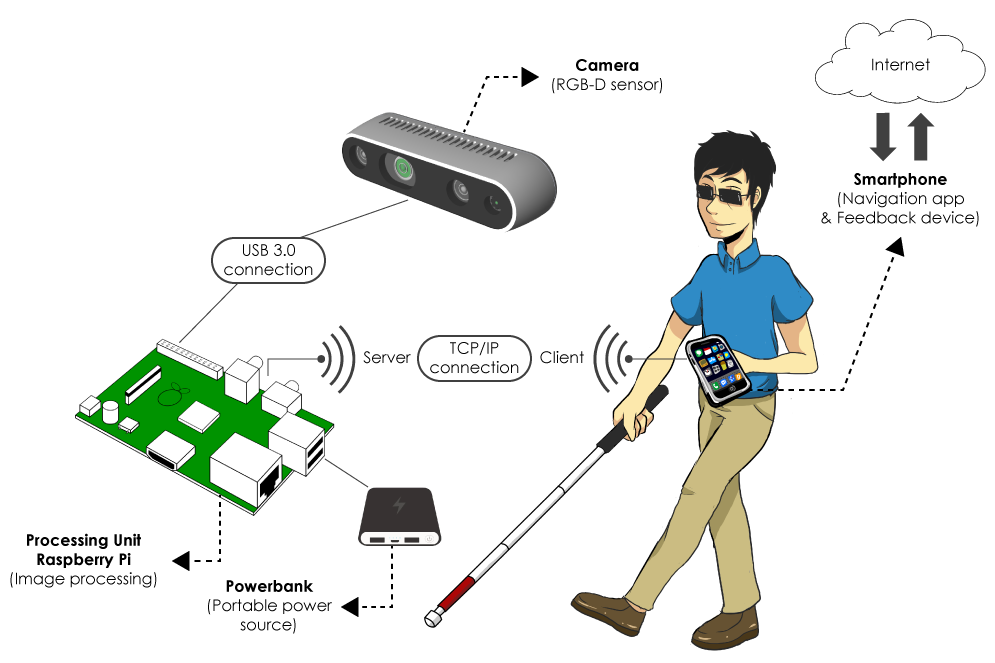
\includegraphics[width=\textwidth]{images/architecture.png}
    \caption{Αρχιτεκτονική προτεινόμενου συστήματος}
    \label{fig:architecture}
\end{figure}

Η αρχιτεκτονική του συστήματος πλοήγησης που προτείνεται στην παρούσα εργασία βασίζεται πάνω σε 3 κύριους πυλώνες:
\begin{itemize}
    \item \textbf{Μια κάμερα RGB-D με ενσωματωμένο αισθητήρα βάθους}: Στην λύση που προτείνουμε χρησιμοποιείται μια κάμερα ως μονάδα "αίσθησης" του εξωτερικού περιβάλλοντος μπροστά από τον χρήστη, η οποία έχει τη δυνατότητα καταγραφής βίντεο σε έγχρωμη μορφή (RGB) και παράλληλα δίνει ως έξοδο έναν χάρτη βάθους (depth map). Ουσιαστικά η κάμερα παίζει τον ρόλο των ματιών και δίνει την δυνατότητα υπολογισμού της απόστασης διαφόρων αντικειμένων από το άτομο με προβλήματα όρασης.
    \item \textbf{Ένα smartphone με εγκατεστημένη την εφαρμογή πλοήγησης}: Ως μέσο αλληλεπίδρασης του χρήστη με το σύστημα επιλέχθηκε το κινητό του. Ο λόγος είναι στην σημερινή εποχή η πλειοψηφία των ανθρώπων, ακόμα κι αυτών με προβλήματα όρασης, είναι εξοικειωμένοι με την χρήση ενός smartphone. Πρόκειται, δηλαδή, για μια συσκευή που ο καθένας έχει ανά πάσα στιγμή πάνω του και δεν προσθέτει επιπλέον φόρτο εργασίας στον χρήστη. Η εφαρμογή που αναπτύχθηκε στα πλαίσια της διπλωματικής εργασίας επιτρέπει στον χρήστη να εισάγει έναν προορισμό και η ίδια αναλαμβάνει την εύρεση της κατάλληλης διαδρομής, λαμβάνοντας υπόψιν την τωρινή τοποθεσία του χρήστη και τα δεδομένα από τους χάρτες πλοήγησης. Γίνεται αξιοποίηση του ενσωματωμένου GPS του κινητού και της εσωτερικής του πυξίδας, που περιλαμβάνει μαγνητόμετρο, γυροσκόπιο και επιταχυνσιόμετρο.
    \item \textbf{Την κύρια μονάδα επεξεργασίας εικόνας}: Για να λειτουργήσει ένα σύστημα πλοήγησης πρέπει να υπάρχει μια μονάδα η οποία θα λαμβάνει το βίντεο από την κάμερα και θα είναι υπεύθυνη για την επεξεργασία εικόνας που απαιτείται. Στην παρούσα εργασία επιλέχθηκε η χρήση ενός Raspberry Pi 4, το οποίο παρέχει την απαραίτητη επεξεργαστική ισχύ που απαιτείται για την επεξεργασία της ροής βίντεο, καθώς επίσης έχει και πολύ μικρό μέγεθος (λίγο μεγαλύτερο από πιστωτική κάρτα), που συμβάλλει στην φορητότητα του συστήματος. Πιο συγκεκριμένα, στο Raspberry Pi "τρέχουν" όλοι οι αλγόριθμοι εντοπισμού και αναγνώρισης εικόνας.
\end{itemize}

\subsection{Πλοήγηση σε αστικό περιβάλλον – δυσκολίες και περιορισμοί}
Όπως έχει ήδη αναφερθεί, στην παρούσα διπλωματική εργασία παρουσιάζεται ένα σύστημα πλοήγησης που προορίζεται για εξωτερικό χώρο και πιο συγκεκριμένα για αστικά περιβάλλοντα. Αν και οι δυσκολίες μετακίνησης είναι εξίσου έντονες και σε εσωτερικού χώρους, επιλέχθηκε η εστίαση σε εξωτερικά περιβάλλοντα, γιατί συνήθως αυτά είναι άγνωστα στους χρήστες και οι κίνδυνοι που μπορεί να αντιμετωπίσουν είναι πιο απρόβλεπτοι. Κατά την υλοποίηση του προτεινόμενου συστήματος πλοήγησης λήφθηκαν υπόψιν οι εξής παρατηρήσεις:
\begin{itemize}
    \item Ο εντοπισμός της θέσης του χρήστη είναι πιο εύκολος λόγω της διαθεσιμότητας του GPS. Αντίθετα, σε έναν εσωτερικό χώρο η χρήση του GPS είναι προβληματική λόγω χαμηλής στάθμης του σήματος.
    \item Σε ένα αστικό περιβάλλον, όπως μεγάλες πόλεις με ψηλά κτήρια, υπάρχει πιθανότητα να έχουμε ελάττωση της στάθμης σήματος του GPS, λόγω της παρεμβολής των κτιρίων. Αυτό οδηγεί συνήθως σε μειωμένη ακρίβεια του GPS, κάτι που είναι κρίσιμο για την πλοήγηση ενός ατόμου με μειωμένη όραση. Συχνά, αυτό το πρόβλημα εξαλείφεται με την κατασκευή όλο και καλύτερων δεκτών GPS, ή αλγοριθμικά με τη χρήση τεχνικών εντοπισμού θέσης μέσω της κάμερας που φέρει ο χρήστης. Στην παρούσα εργασία δεν θα ασχοληθούμε με την επίλυση του συγκεκριμένου ζητήματος, καθώς είναι κάτι που ξεφεύγει από τους στόχους.
    \item Κατά την πλοήγησή του ο χρήστης θα βρεθεί, συχνά, αντιμέτωπος με διάφορα φυσικά αντικείμενα, που λειτουργούν ως εμπόδια στην διαδρομή του. Επίσης, η ελλιπής συντήρηση των υποδομών, όπως η ύπαρξη σπασμένων πλακιδίων ή φυτών στα πεζοδρόμια και η έλλειψη ανάγλυφων οδηγών για τους τυφλούς, δυσχεραίνει την μετακίνησή των ατόμων αυτών.
    \item Τέλος, τα συστήματα πλοήγησης που βασίζονται σε κάμερες ή αισθητήρες υπερύθρων, επηρεάζονται από τις ακτίνες του ήλιου, οι οποίες δημιουργούν παρεμβολές και περιορίζουν την εφαρμοσιμότητα των αλγορίθμων.
\end{itemize}

\subsection{Παράλληλη χρήση με το λευκό μπαστούνι}
Αν και η τεχνολογία έχει πραγματοποιήσει τεράστια άλματα προόδου τις τελευταίες δεκαετίες, είναι γεγονός πως δεν έχει σχεδιαστεί κάποια εφαρμογή πλοήγησης για τυφλούς που να ικανοποιεί τις ανάγκες τους πλήρως και να αντικαταστήσει τις παραδοσιακές μεθόδους υποβοήθησης πλοήγησης \cite{LowVisio34:online}. Συνεπώς, η κοινότητα των ατόμων με προβλήματα όρασης εξακολουθεί δικαίως να χρησιμοποιεί το λευκό μπαστούνι, ως το κύριο βοήθημα μετακίνησης, κάτι το οποίο δεν μπορεί να αλλάξει από τη μια στιγμή στην άλλη. Για αυτόν τον λόγο, το σύστημα που παρουσιάζεται στην παρούσα εργασία προορίζεται να λειτουργεί υποστηρικτικά στη χρήση του λευκού μπαστουνιού, βελτιώνοντας ταυτόχρονα την εμπειρία μετακίνησης των χρηστών και επιτρέποντάς τους την χρήση των εργαλείων που εμπιστεύονται και με τα οποία έχουν εξοικειωθεί.

\section{Απτική Ανάδραση}
\subsection{Αισθητηριακή υποκατάσταση}
Η έννοια της αισθητηριακής υποκατάστασης (sensory substitution) αναφέρεται στην τροποποίηση ορισμένων χαρακτηριστικών ενός αντιληπτικού συστήματος (π.χ. όραση, ακοή, αφή, όσφρηση, γεύση) και η μετατροπή τους σε ερεθίσματα για ένα διαφορετικό αντιληπτικό σύστημα \cite{wiki:sensory_sub}. Με άλλα λόγια, η κεντρική ιδέα της αισθητηριακής υποκατάστασης είναι ότι οι πληροφορίες, οι οποίες δεν είναι διαθέσιμες σε κάποιον εξαιτίας μιας αισθητηριακής διαταραχής, μπορούν να γίνουν αντιληπτές μέσω ενός άλλου αντιληπτικού συστήματος. Η μετατροπή, ωστόσο, των ερεθισμάτων από ένα αντιληπτικό σύστημα σε ένα άλλο είναι μια πολύπλοκη διαδικασία με πολλές παραμέτρους, η οποία αποτελεί αντικείμενο έρευνας τόσο στον ιατρικό όσο και στον τεχνολογικό τομέα. Στα πλαίσια της διπλωματικής εργασίας θα αξιοποιήσουμε πολύ βασικές γνώσεις που αφορούν την αντικατάσταση μιας αίσθησης με μια άλλη, χωρίς να εμβαθύνουμε περαιτέρω.

\subsection{Υπάρχοντα κανάλια μετάδοσης χωρικής πληροφορίας}
Οι άνθρωποι με φυσιολογική όραση χρησιμοποιούν την όραση για να προσδιορίσουν την θέση τους και το μονοπάτι στο οποίο θα κινηθούν. Τα άτομα με προβλήματα όρασης έχουν αναπτύξει τις υπόλοιπες αισθήσεις τους ώστε να μπορούν να αντιλαμβάνονται τον χώρο στον οποίο βρίσκονται. Όπως είναι φυσιολογικό τα δύο αισθητήρια κανάλια που αξιοποιούνται περισσότερο είναι το ακουστικό και το απτικό, το οποίο έχει επιβεβαιωθεί κι από αντίστοιχες έρευνες \cite{schmidt2013spatial}. Χρησιμοποιώντας το ακουστικό κανάλι τα άτομα με προβλήματα όρασης είναι σε θέση να αντιλαμβάνονται τις αλλαγές που συμβαίνουν γύρω τους και να προσανατολίζονται, χρησιμοποιώντας διάφορες πηγές ήχου ως σημεία αναφοράς, π.χ. ο θόρυβος που κάνουν τα οχήματα τους επιτρέπει να γνωρίζουν πού βρίσκεται ο δρόμος, ενώ η ηχητική ειδοποίηση των φαναριών τους βοηθάει να καταλάβουν αν είναι πράσινο ή κόκκινο. Αντίθετα, η χωρική πληροφορία είναι δύσκολο να μεταφερθεί άμεσα μέσω του απτικού καναλιού. Η χρησιμότητά του είναι ότι μέσω της αφής ο χρήστης αντιλαμβάνεται περισσότερες λεπτομέρειες σχετικά με την υφή ή το είδος ενός φυσικού αντικειμένου. Για παράδειγμα, όταν ο τυφλός χρησιμοποιεί το λευκό μπαστούνι και αυτό πέσει πάνω σε ένα εμπόδιο, τότε, αναλόγως την δύναμη που ασκείται στον μπαστούνι, μπορεί να αντιληφθεί αν το αντικείμενο αυτό είναι κάτι σκληρό και αμετακίνητο (π.χ. μια κολόνα δημοτικού φωτισμού), ή κάτι πιο εύκαμπτο και μετακινήσιμο (π.χ. μια καρέκλα).

\subsection{Γιατί απτική ανάδραση;}
Στην παρούσα διπλωματική εργασία υλοποιείται ένα σύστημα υποβοήθησης πλοήγησης που βασίζεται στην απτική αλληλεπίδραση με τον χρήστη. Πιο συγκεκριμένα, υλοποιήθηκε ένα σύστημα που ειδοποιεί τον χρήστη μέσω δονήσεων για το πότε και πού πρέπει να κινηθεί, καθώς επίσης και όταν απαιτείται η διάσχιση ενός δρόμου. Η επιλογή του απτικού καναλιού ως μέσο μετάδοσης της χωρικής πληροφορίας έγινε για τους εξής δύο λόγους:
\begin{enumerate}
    \item Το ακουστικό κανάλι είναι ήδη αρκετά επιβαρυμένο με άλλες λειτουργίες \cite{bharadwaj2017tactile, shingledecker1978human} και απαιτείται μια αποσυμφόρηση, ώστε το άτομο με προβλήματα όρασης να μπορεί να αντιλαμβάνεται άλλες κρίσιμες πληροφορίες μέσω της ακοής, π.χ. τον ήχο από τα αυτοκίνητα ή κάποιον περαστικό. Επίσης, η παροχή ανάδρασης μέσω ήχου θα μπορούσε να συγχύσει και να κουράσει πνευματικά τον χρήστη, λόγω πολλών παράλληλων ακουστικών ερεθισμάτων.
    \item Η χρήση δονήσεων αποτελεί έναν πιο διακριτικό τρόπο να ενημερώνεται ο χρήστης για πληροφορίες που αφορούν το εξωτερικό περιβάλλον. Η διακριτικότητα και η ευκολία είναι από τα βασικά χαρακτηριστικά του προτεινόμενου συστήματος και η αξιοποίηση του απτικού καναλιού είναι απαραίτητη για να επιτευχθεί κάτι τέτοιο.
\end{enumerate}

\subsection{Haptic icons}
Ως haptic icons ορίζονται στην βιβλιογραφία τα διάφορα απτά ερεθίσματα στα οποία έχουμε αποδώσει συγκεκριμένα νοήματα (π.χ. ένα απτικό ερέθισμα μπορεί να είναι "συνδεδεμένο" με την έκφραση χαράς, λύπης κλπ.) \cite{chan2008designing}. Σχετικές έρευνες \cite{seifi2017exploiting, shieh2008tactile} έχουν μελετήσει τη σχέση μεταξύ των απτικών ερεθισμάτων που δέχεται ένας άνθρωπος και των συναισθημάτων που του προκαλούν. Συνήθως συστήματα που βασίζονται στην αξιοποίηση του απτικού καναλιού στοχεύουν στην μετάδοση πληροφοριών στον χρήστη μέσω της χρήσης διαφορετικών μοτίβων δονήσεων, τα οποία είναι συνδεδεμένα με διαφορετικές εντολές πλοήγησης. Τα διαφορετικά μοτίβα δονήσεων μπορεί να περιλαμβάνουν διαφορές στην ένταση της δόνησης, στην αλληλουχία των δονήσεων και στην συχνότητά τους. Για τις ανάγκες της συγκεκριμένης διπλωματικής εργασίας χρησιμοποιήθηκε η λογική της αντιστοίχησης ενός μοτίβου δονήσεων, τα οποία παίζουν τον ρόλο των haptic icons, για κάθε διαφορετική εντολή που απαιτείται από τον χρήστη. Κάθε μοτίβο έχει το ίδιο επίπεδο έντασης, καθώς θεωρήθηκε ότι ο αριθμός των εντολών που έπρεπε να κωδικοποιηθούν δεν ήταν τόσο μεγάλος, ώστε να αξιοποιηθεί και η ένταση των δονήσεων για περισσότερη διακριτοποίηση. Πιο συγκεκριμένα:
\begin{itemize}
    \item Εντολή \textbf{"Στρίψε Αριστερά"}: Η εντολή αυτή ειδοποιεί τον χρήστη ότι πρέπει να πραγματοποιήσει στροφή αριστερά 90\degree. Το μοτίβο δονήσεων που αντιστοιχεί σε αυτήν την εντολή είναι "σύντομη δόνηση - μικρή παύση - σύντομη δόνηση".
    \item Εντολή \textbf{"Στρίψε Δεξιά"}: Η εντολή αυτή ειδοποιεί τον χρήστη ότι πρέπει να πραγματοποιήσει στροφή δεξιά 90\degree. Το μοτίβο δονήσεων που αντιστοιχεί σε αυτήν την εντολή είναι "μακρά δόνηση - μικρή παύση - μακρά δόνηση".
    \item Εντολή \textbf{"Σταμάτα"}: Η εντολή αυτή ειδοποιεί τον χρήστη ότι πρέπει να σταματήσει μπροστά από μια διάβαση, επειδή το ο φωτεινός σηματοδότης είναι κόκκινος. Το μοτίβο δονήσεων που αντιστοιχεί σε αυτήν την εντολή είναι "πολύ μακρά δόνηση - πολύ σύντομη παύση".
    \item Εντολή \textbf{"Προχώρα"}: Η εντολή αυτή ειδοποιεί τον χρήστη ότι μπορεί να διασχίσει μια διάβαση, επειδή το ο φωτεινός σηματοδότης είναι πράσινος. Το μοτίβο δονήσεων που αντιστοιχεί σε αυτήν την εντολή είναι "σύντομη δόνηση - πολύ σύντομη παύση - μακρά δόνηση - πολύ σύντομη παύση".
\end{itemize}
\begin{figure}[H]
    \centering
    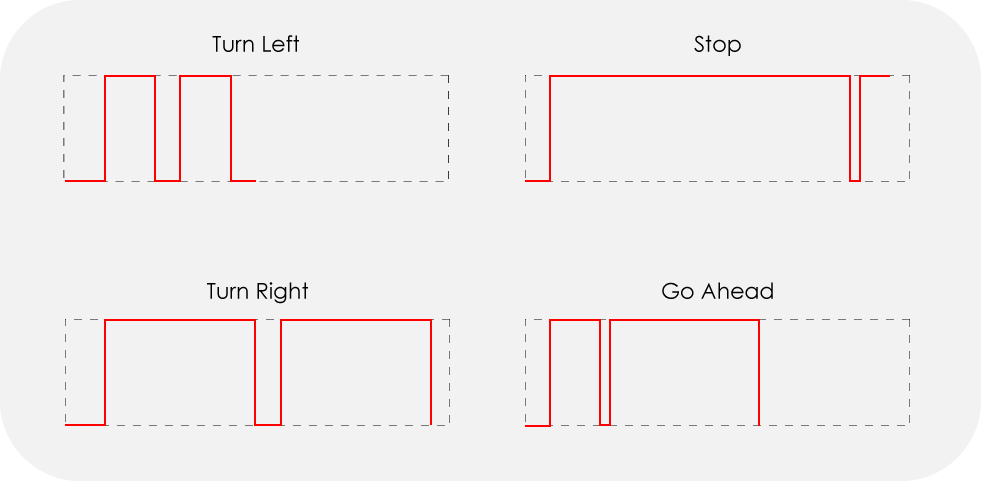
\includegraphics[width=\textwidth]{images/haptic_icons.png}
    \caption{Αντιστοίχηση μοτίβων δονήσεων σε εντολές πλοήγησης}
    \label{fig:haptic-icons}
\end{figure}

\subsection{Δυνατότητες και περιορισμοί}
Όπως έχουμε ήδη αναφέρει η χρήση της αφής ως μέσο μετάδοσης πληροφορίας έχει πολύ μεγάλο πλεονέκτημα την διακριτικότητα και την αμεσότητα στην αντίληψη της πληροφορίας. Ωστόσο, συγκριτικά με την ακοή, προβάλει ένα σημαντικό μειονέκτημα, το οποίο είναι η χαμηλή διακριτότητα της πληροφορίας που μπορεί να μεταδοθεί \cite{kaczmarek1991electrotactile}. Με απλά λόγια, αν θέλουμε να κωδικοποιήσουμε πολλές διαφορετικές εντολές με χρήση μοτίβων δονήσεων, τότε θα πρέπει να δημιουργήσουμε ένα διαφορετικό μοτίβο για κάθε ξεχωριστή εντολή. Ωστόσο, η δυνατότητα του ανθρώπου να αντιλαμβάνεται διαφορετικά μοτίβα δονήσεων με μικρές διαφορές μεταξύ τους μειώνεται όσο αυξάνεται η πολυπλοκότητα και ο αριθμός αυτών των μοτίβων. Έρευνες έχουν δείξει επίσης, ότι η διακριτότητα της πληροφορίας που μπορεί να αντιληφθεί ένα άνθρωπος μέσω της αφής εξαρτάται από το σημείο του δέρματος που δέχεται τη διέγερση, για παράδειγμα τα δάκτυλα έχουν πολύ μεγαλύτερη δυνατότητα διάκρισης σε σχέση με τον αγκώνα. Το κατώφλι διάκρισης μεταξύ δυο σημείων (two-point discrimination threshold (TPDT)) ορίζεται ως το μέτρο το οποίο αναπαριστά πόσο πρέπει να απέχουν δυο σημεία πίεσης ώστε να θεωρηθούν από το δέρμα ως διακριτά \cite{koo2016two}.
\begin{figure}[H]
    \centering
    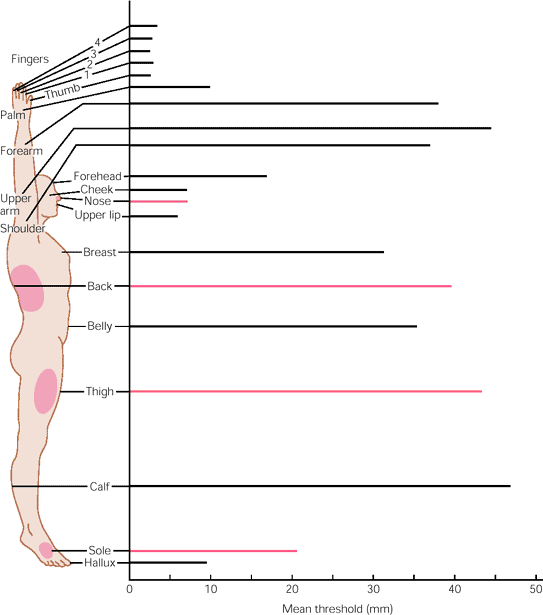
\includegraphics[width=0.6\textwidth]{images/TPDT.png}
    \caption{Μεταβολή του TPDT σε συνάρτηση με τα σημεία του σώματος \cite{weinstein1968intensive}}
    \label{fig:TPDT}
\end{figure}
\newpage
\section{Εξοπλισμός - Υλικό (Hardware)}
Στην ενότητα αυτή θα γίνει μια πλήρης περιγραφή του εξοπλισμού που χρησιμοποιήθηκε στα πλαίσια της παρούσας διπλωματικής εργασίας.

\subsection{Μονάδα «αίσθησης» του περιβάλλοντος – Camera/Depth Sensor}
\subsubsection{Διαθέσιμοι αισθητήρες}
Υπάρχουν πολλοί διαθέσιμοι αισθητήρες-κάμερες που θα μπορούσαν να αξιοποιηθούν στα πλαίσια ενός συστήματος πλοήγησης για άτομα με προβλήματα όρασης. Η επιλογή του κατάλληλου αισθητήρα εξαρτάται κυρίως από τις ανάγκες τις εκάστοτε εφαρμογής, π.χ. αν πρόκειται για εξωτερικό ή εσωτερικό περιβάλλον κλπ. Στην παρούσα εργασία χρησιμοποιήσαμε την κάμερα \emph{Intel Realsense D435i}, ωστόσο πριν προχωρήσουμε στην τελική επιλογή κάμερας εξετάσαμε τις εξής εναλλακτικές επιλογές:
\begin{itemize}
    \item \emph{ZED Stereo Camera}: Πρόκειται για μια κάμερα που λειτουργεί με την μέθοδο της στερεοσκοπικής όρασης, δηλαδή χρησιμοποιεί δύο διαφορετικούς φακούς με οριζόντια απόσταση ο ένας από τον άλλο, και το βάθος/απόσταση υπολογίζεται συγκρίνοντας την μετατόπιση των δύο διαφορετικών εικόνων.
    \begin{table}[H]
    \centering
    \begin{tabular}{|c|c|}
        \hline
        Technology: & Stereo Depth Sensing\\
        \hline
        Field of View (FoV): & Max. 90°(H) x 60°(V) x 100°(D)\\
        \hline
        RGB Sensor Type: & 1/3” 4MP CMOS\\
        \hline
        Depth Range: & 0.5m to 25m\\
        \hline
        Depth FPS: & Up to 100Hz\\
        \hline
        Depth Accuracy: & <= 2\% up to 3m, <= 4\% up to 15m\\
        \hline
        Dimensions: & 175 x 30 x 33 mm\\ 
        \hline
        Power: & 380mA / 5V USB Powered\\
        \hline
        SDK Provided: & YES\\
        \hline
    \end{tabular}
    \caption{Χαρακτηριστικά ZED Stereo Camera \cite{ZEDStere94:online}}
    \label{tab:zed}
    \end{table}
    \begin{figure}[H]
        \centering
        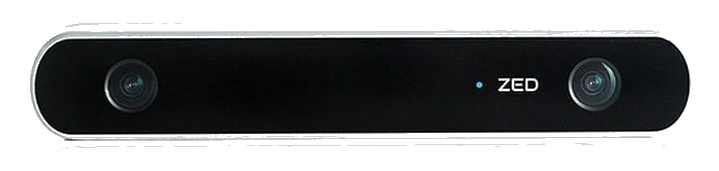
\includegraphics[width=0.6\textwidth]{images/zed.png}
        \caption{ZED Stereo Camera}
        \label{fig:zed}
    \end{figure}

    \item \emph{CamBoard pico flexx depth sensor}: Ο αισθητήρας αυτός είναι από τους πιο μικρούς που υπάρχουν και χρησιμοποιεί την τεχνολογία Time-of-Flight (ToF), με εκπομπή υπέρυθρης ακτινοβολίας, για να υπολογίσει την απόσταση των αντικειμένων, χωρίς ωστόσο να παρέχει δυνατότητα RGB εικόνας.
    \begin{table}[H]
    \centering
    \begin{tabular}{|c|c|}
        \hline
        Technology: & Time-of-Flight (ToF)\\
        \hline
        Field of View (FoV): & Max. 62°(H) x 45°(V)\\
        \hline
        RGB Sensor Type: & Δεν υποστηρίζεται\\
        \hline
        Depth Range: & 0.1m to 4m\\
        \hline
        Depth FPS: & Up to 45fps\\
        \hline
        Depth Accuracy: & <= 1\% of distance (0.5 – 4m @ 5fps), <= 2\% of distance (0.1 – 1m @ 45fps)\\
        \hline
        Dimensions: & 68 x 17 x 7.35 mm\\ 
        \hline
        Power: & 300mW / USB2.0 compliant\\
        \hline
        SDK Provided: & YES\\
        \hline
    \end{tabular}
    \caption{Χαρακτηριστικά CamBoard pico flexx depth sensor \cite{CamBoard10:online}}
    \label{tab:pico}
    \end{table}
    \begin{figure}[H]
        \centering
        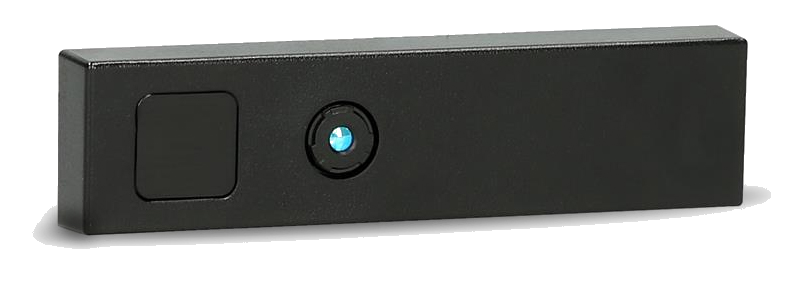
\includegraphics[width=0.6\textwidth]{images/pico_flexx.png}
        \caption{CamBoard pico flexx depth sensor}
        \label{fig:pico}
    \end{figure}
\end{itemize}

\subsubsection{Κριτήρια επιλογής κατάλληλου αισθητήρα}
Η επιλογή του κατάλληλου αισθητήρα έγινε λαμβάνοντας υπόψιν τα παρακάτω κριτήρια:
\begin{enumerate}
    \item \emph{Διαστάσεις κάμερας}: Στόχος είναι η φορητότητα και η διακριτικότητα του συστήματος, άρα θέλουμε έναν όσο γίνεται μικρότερο σε διαστάσεις αισθητήρα.
    \item \emph{Ταυτόχρονη υποστήριξη RGB \& Depth Frames}: Η προτεινόμενη εφαρμογή αξιοποιεί τόσο την έγχρωμη εικόνα RGB για την αναγνώριση της διάβασης πεζών και των φωτεινών σηματοδοτών, όσο και τον χάρτη βάθους (depth map) για τον εντοπισμό φυσικών εμποδίων.
    \item \emph{Ανθεκτικότητα στις συνθήκες φωτισμού}: Λόγω της φύσης του συστήματος, είναι απαραίτητο η κάμερα να αποδίδει επαρκώς καλά τόσο σε εσωτερικά, όσο και σε εξωτερικά περιβάλλοντα. Ιδιαίτερα η ακρίβεια των μετρήσεων της κάμερας σε εξωτερικό περιβάλλον επηρεάζεται από τον φωτισμό του περιβάλλοντος και τον προσανατολισμό της σε σχέση με τις ακτίνες του ήλιου. 
    \item \emph{Επαρκή υποστήριξη με SDK (Software Development Kit)}: Κατά την υλοποίηση μιας εργασίας είναι πολύ σημαντικό να υπάρχουν διαθέσιμα παραδείγματα κώδικα και έτοιμες συναρτήσεις που διευκολύνουν την ανάπτυξη των αλγορίθμων. Τα SDKs είναι πακέτα λογισμικού, που περιέχουν βελτιστοποιημένες συναρτήσεις και βασικά παραδείγματα για την ορθή χρήση του εκάστοτε αισθητήρα. Η ύπαρξη μιας ευρύτερης κοινότητας γύρω από έναν συγκεκριμένο αισθητήρα συμβάλλει στην πιο γρήγορη και αποτελεσματική υλοποίηση, καθώς και στην πιο εύκολη επίλυση των σφαλμάτων.
    \item \emph{Ακρίβεια και εύρος μέτρησης απόστασης}: Η ακρίβεια κατά την μέτρηση των αποστάσεων, καθώς και το εύρος της μέτρησης (ελάχιστη/μέγιστη μετρήσιμη απόσταση) είναι κρίσιμα κριτήρια για την επιλογή του κατάλληλου αισθητήρα βάθους, ο οποίος θα καλύπτει τις ανάγκες ενός πεζού χρήστη με προβλήματα όρασης.
\end{enumerate}

\subsubsection{Intel RealSense D435i}
Στα πλαίσια της παρούσας διπλωματικής εργασίας χρησιμοποιήθηκε η κάμερα \emph{Intel Realsense D435i}, η οποία περιέχει έναν RGB φακό και έναν ενσωματωμένο αισθητήρα βάθους, ο οποίος λειτουργεί με στερεοσκοπική όραση. Η αρχή λειτουργίας της στερεοσκοπικής όρασης είναι παρόμοια με τον τρόπο που αντιλαμβάνεται το βάθος ο ανθρώπινος εγκέφαλος μέσω των ματιών, δηλαδή υπάρχουν δύο φακοί-αισθητήρες τοποθετημένοι σε μικρή απόσταση μεταξύ τους και λαμβάνουν δύο διαφορετικές εικόνες ενός αντικειμένου. Συγκρίνοντας τις δύο εικόνες και γνωρίζοντας την απόσταση μεταξύ των δύο φακών εξάγεται η πληροφορία που αφορά το βάθος (Σχήμα \ref{fig:stereo}). Οι στερεοσκοπικές κάμερες λειτουργούν αρκετά καλά κάτω από οποιεσδήποτε συνθήκες φωτισμού, αφού το βάθος υπολογίζεται αποκλειστικά από την σύγκριση εικόνων. Η κάμερα Intel Realsense D435i χρησιμοποιεί επιπλέον έναν πομπό υπέρυθρης ακτινοβολίας (infrared projector), ώστε έχει μεγαλύτερη ακρίβεια μετρήσεων σε περιβάλλοντα χαμηλού φωτισμού. Τέλος, ενσωματώνει κι έναν IMU (Inertial Measurement Sensor) sensor, έναν αισθητήρα που περιλαμβάνει επιταχυνσιόμετρο και γυροσκόπιο, για να μετράει την περιστροφή και τον προσανατολισμό της κάμερας με 6 βαθμούς ελευθερίας.

\begin{figure}[H]
        \centering
        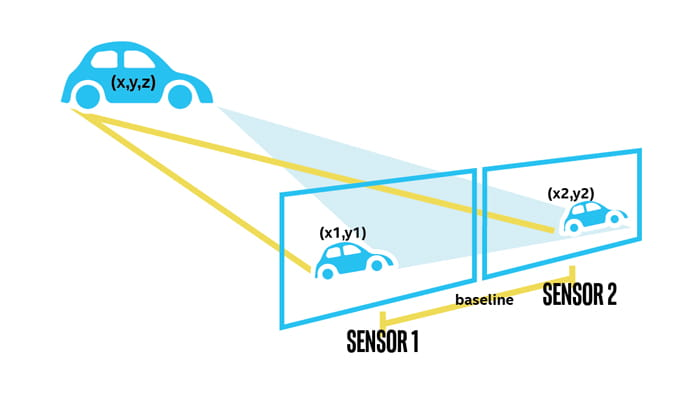
\includegraphics[width=0.8\textwidth]{images/how_stereo_depth_works.jpg}
        \caption{Αρχή λειτουργίας στερεοσκοπικής όρασης}
        \label{fig:stereo}
    \end{figure}

\begin{table}[H]
    \centering
    \begin{tabular}{|c|c|}
        \hline
        Technology: & Active IR Stereo\\
        \hline
        Field of View (FoV): & Max. 90°(H) x 59°(V) x 98°(D)\\
        \hline
        RGB Sensor: & 1920 x 1080, 30fps\\
        \hline
        Depth Range: & 0.105m to 10m\\
        \hline
        Depth FPS: & Up to 90fps\\
        \hline
        Dimensions: & 90 x 25 x 25 mm\\ 
        \hline
        Power: & USB3.0\\
        \hline
        SDK Provided: & YES\\
        \hline
    \end{tabular}
    \caption{Χαρακτηριστικά Intel Realsense D435i \cite{DepthCam34:online}}
    \label{tab:realsense}
\end{table}
\begin{figure}[H]
    \centering
    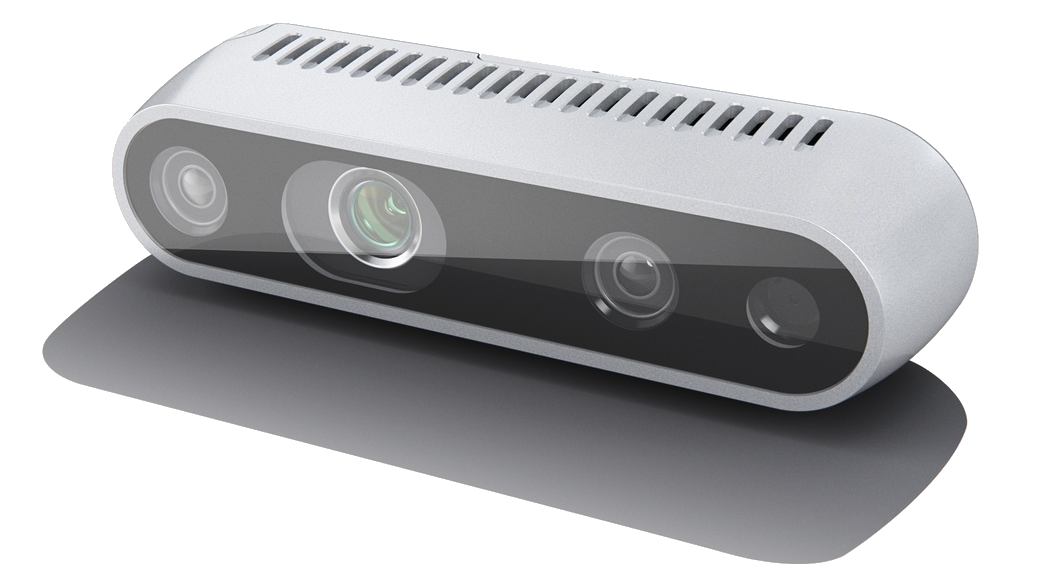
\includegraphics[width=0.8\textwidth]{images/intel_realsense.png}
    \caption{Intel Realsense Depth Camera D435i}
    \label{fig:realsense}
\end{figure}
\begin{figure}[H]
    \centering
    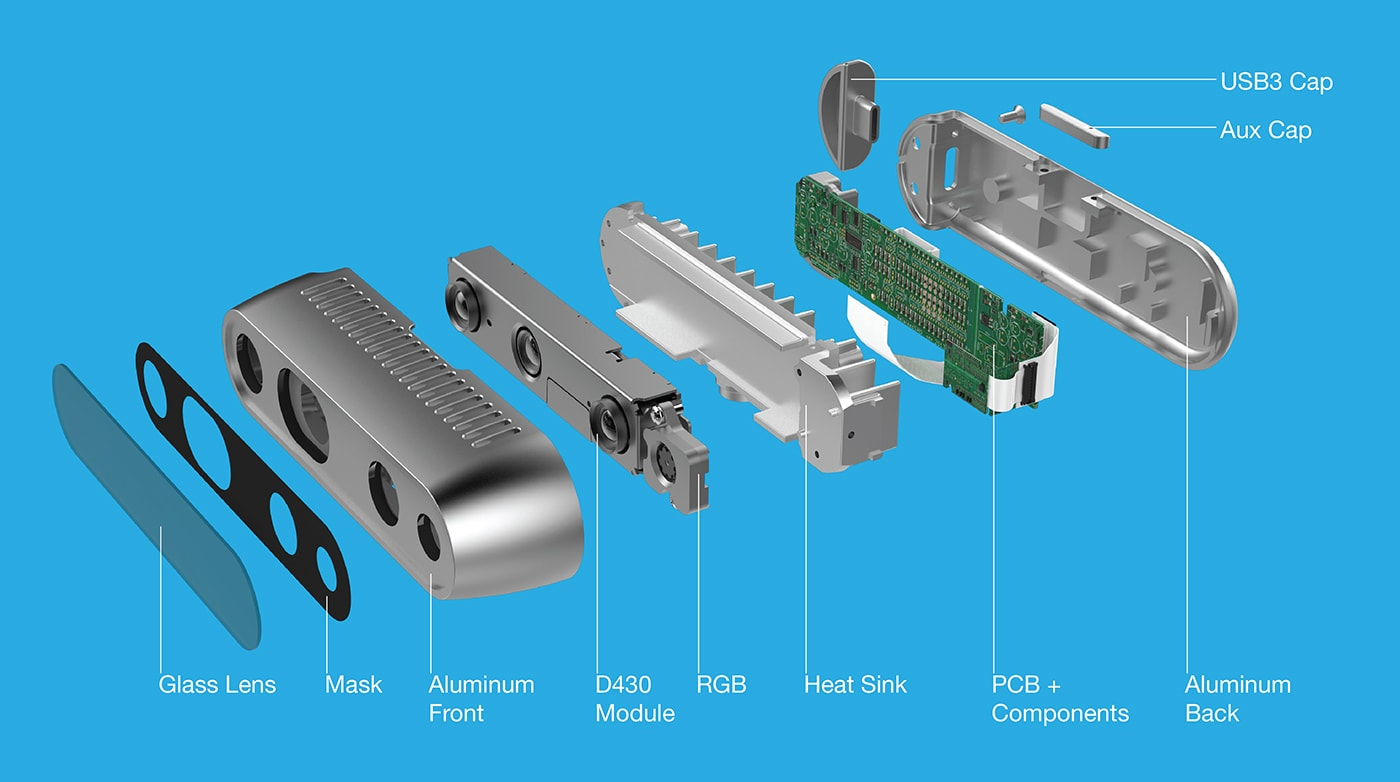
\includegraphics[width=\textwidth]{images/d435_inside_depth_camera.jpg}
    \caption{Intel Realsense D435i - Εσωτερική δομή}
    \label{fig:realsense-inside}
\end{figure}

\subsection{Μονάδα επεξεργασίας εικόνας – Μικροϋπολογιστής}
Οι αλγόριθμοι εντοπισμού και αναγνώρισης αντικειμένων χρησιμοποιούν τεχνικές επεξεργασίας εικόνας για να καταφέρουν να αποκωδικοποιήσουν μια φωτογραφία ή ένα βίντεο. Η επεξεργασία εικόνας και βίντεο είναι μια απαιτητική εργασία τόσο σε μνήμη όσο και σε επεξεργαστική ισχύ, επομένως είναι απαραίτητη η ύπαρξη ενός υπολογιστή ή κάποιας μονάδας επεξεργασίας που θα μπορεί να αντεπεξέλθει στις απαιτήσεις αυτές.

\subsubsection{Raspberry Pi 4}
\begin{figure}[H]
    \centering
    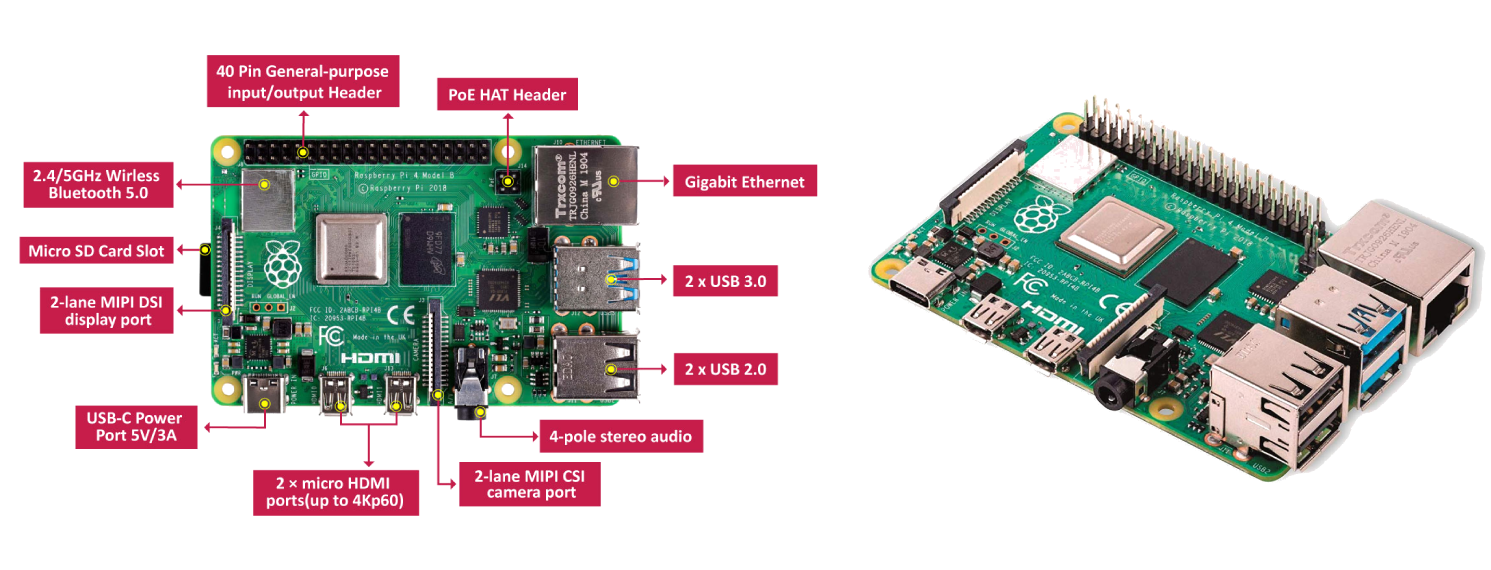
\includegraphics[width=\textwidth]{images/raspberry.png}
    \caption{Raspberry Pi 4 Model B}
    \label{fig:RPi4modelB}
\end{figure}
Για τις ανάγκες της διπλωματικής εργασίας επιλέχθηκε η χρήση του μικροεπεξεργαστή \emph{Raspberry Pi 4} (RPi4). Το RPi4 είναι ένας πλήρης υπολογιστής σε μέγεθος πιστωτικής κάρτας, στον οποίο μπορούν να συνδεθούν διάφορες περιφερειακές συσκευές, όπως πληκτρολόγιο, οθόνη κλπ. Πιο συγκεκριμένα, χρησιμοποιήθηκε η έκδοση Model B του Raspberry Pi 4, το οποίο έχει βελτιωμένα χαρακτηριστικά, όπως υποστήριξη USB3.0, μεγαλύτερη μνήμη RAM (4GB) και καλύτερο επεξεργαστή γραφικών. Στον πίνακα \ref{tab:raspberry} παρουσιάζονται αναλυτικά τα χαρακτηριστικά του Raspberry Pi 4 που χρησιμοποιήσαμε.

\begin{table}[H]
    \centering
    \begin{tabular}{|c|c|}
        \hline
        Processor: & Broadcom BCM2711, quad-core Cortex-A72 (ARM v8)
64-bit SoC @ 1.5GHz\\
        \hline
        Memory: & 4GB LPDDR4\\
        \hline
        Connectivity: & WLAN, Ethernet, Bluetooth 5.0, BLE\\
        \hline
        USB2.0: & 2 ports\\
        \hline
        USB3.0: & 2 ports\\
        \hline
        HMDI: & 2 micro HDMI ports\\
        \hline
        Micro SD: & YES\\
        \hline
        Input power: & 5V DC via USB-C connector (minimum 3A)\\
        \hline
    \end{tabular}
    \caption{Χαρακτηριστικά Raspberry Pi 4 Model B \cite{BuyaRasp17:online}}
    \label{tab:raspberry}
\end{table}

Ουσιαστικά, στα πλαίσια της παρούσας εργασίας αξιοποιήθηκαν κυρίως η μεγάλη χωρητικότητα μνήμης RAM και η ύπαρξη θύρας USB3.0, μιας και η κάμερα που επιλέξαμε υποστήριζε αποκλειστικά USB3.0 interface. Ταυτόχρονα, η μεγάλη επεξεργαστική ισχύς συνέβαλε στο να τρέχει ο αλγόριθμος σε real-time, ενώ η WiFi συνδεσιμότητα επέτρεψε την σύνδεση με τα άλλα μέρη του συστήματος, όπως θα δούμε παρακάτω. Η τροφοδοσία του RPi4 μπορεί να γίνει με δύο τρόπους: είτε με μια συστοιχία από μπαταρίες ιόντων λιθίου, είτε μέσω ενός powerbank (φορητή μπαταρία). Επιλέχθηκε η δεύτερη λύση του powerbank, καθώς ήταν πολύ πιο εύκολο να το αποκτήσουμε και δεν απαιτεί ιδιαίτερους χειρισμούς όσον αφορά την επαναφόρτισή του. Το RPi4 απαιτεί τροφοδοσία 5V/3A, επομένως χρησιμοποιήθηκε ένα powerbank που έχει ως έξοδο 5V/3A και χωρητικότητα μπαταρίας 10.000mAh (Σχήμα \ref{fig:powerbank}). Η αυτονομία του συστήματος με την χρήση της συγκεκριμένης φορητής μπαταρίας φτάνει έως και την 1.5 ώρα.

\begin{figure}[H]
    \centering
    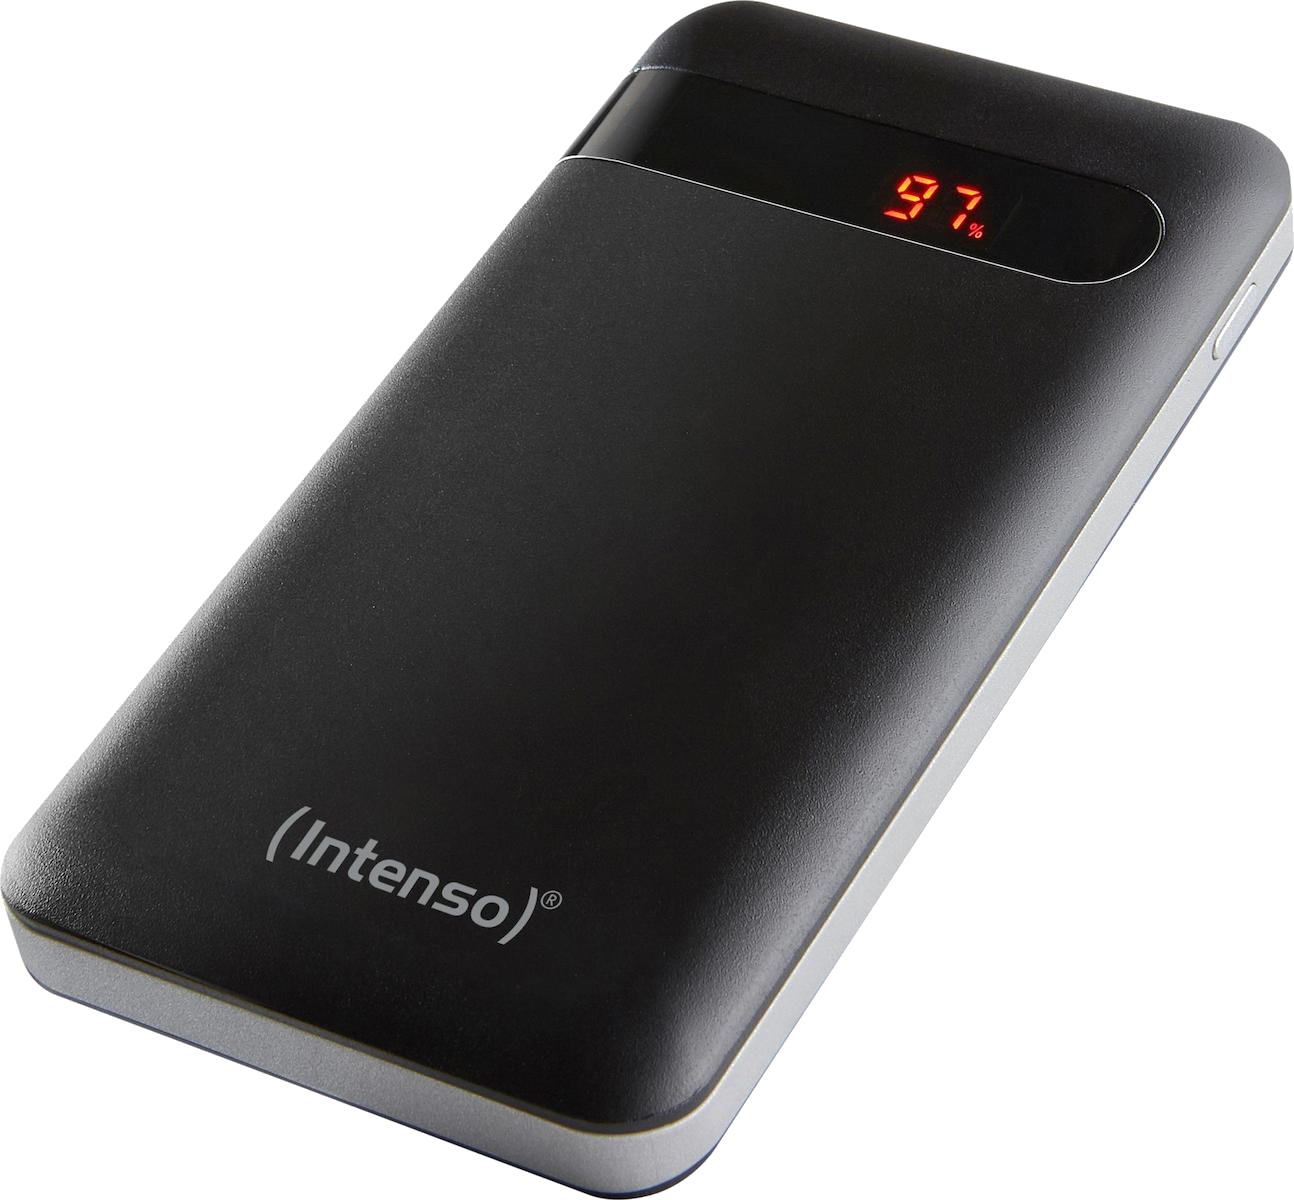
\includegraphics[width=0.6\textwidth]{images/powerbank.png}
    \caption{Το powerbank \emph{Intenso PD10000} που χρησιμοποιήθηκε}
    \label{fig:powerbank}
\end{figure}

\subsection{Συσκευή πλοήγησης – Android Smartphone}
Η επιλογή του κινητού του χρήστη ως κύρια συσκευή πλοήγησης έγινε, διότι πρόκειται για μια συσκευή με την οποία οι χρήστες είναι αρκετά εξοικειωμένοι, είναι άμεσα διαθέσιμη σχεδόν σε όλους και είναι πολύ εύκολο να αναπτυχθούν εφαρμογές για smartphone.

\subsubsection{Εφαρμογή πλοήγησης}
Στα πλαίσια της διπλωματικής αναπτύχθηκε ειδική εφαρμογή για κινητά σε λειτουργικό Android. Η εφαρμογή προορίζεται να εγκαθίσταται στο κινητό του χρήστη και αποτελεί την μοναδική διεπιφάνεια αλληλεπίδρασης του χρήστη με το σύστημα πλοήγησης. Το κομμάτι της υλοποίησης της εφαρμογής περιλαμβάνει την ανάπτυξη κώδικα που αξιοποιεί τους ενσωματωμένους αισθητήρες GPS, IMU και πυξίδα για να μπορεί να εντοπίζεται η τοποθεσία του χρήστη.
\newline
\newline
\textbf{Αρχή λειτουργίας}:

Η εφαρμογή ενσωματώνει έναν χάρτη της ευρύτερης περιοχής χάρη στη χρήση του \emph{Google Maps SDK} \url{https://developers.google.com/maps/documentation/android-sdk/intro}.
Ο χρήστης εισάγει έναν προορισμό στην εφαρμογή και η αντίστοιχη τοποθεσία βρίσκεται μέσω του \emph{Google Places API} (\url{https://developers.google.com/places/web-service/intro}).
Αφού ο χρήστης εισάγει έναν προορισμό, το σύστημα βρίσκει την βέλτιστη διαδρομή, χρησιμοποιώντας το \emph{Google Directions API} (\url{https://developers.google.com/maps/documentation/directions/intro}) και επιστρέφονται ως δεδομένα οι οδηγίες κατεύθυνσης για πεζούς. Το format των οδηγιών είναι JSON, οπότε αναπτύχθηκε μια εσωτερική συνάρτηση στην εφαρμογή που αποκωδικοποιεί τα δεδομένα κατεύθυνσης και τα εξάγει ως μια λίστα από απλές εντολές στροφής (turn-by-turn navigation).
Καθόσον η εφαρμογή βρίσκεται σε λειτουργία πυξίδας, επικοινωνεί με το Raspberry Pi ασύρματα και λαμβάνει εντολές για το αν έχει βρεθεί κάποιο εμπόδιο ή έχει εντοπιστεί διάβαση πεζών. Η εφαρμογή αντιλαμβάνεται τον προσανατολισμό του χρήστη εκμεταλλευόμενη τους εσωτερικούς αισθητήρες του κινητού και υπολογίζει την γωνία απόκλισης που έχει σε σχέση με τον προσανατολισμό του μονοπατιού που ακολουθεί. Αν η απόκλιση είναι μεγαλύτερη των 30\degree (σχήμα \ref{fig:degree-orientation}), τότε τον ειδοποιεί κατάλληλα (με χρήση δονήσεων για στροφή αριστερά ή δεξιά).
\begin{figure}[H]
    \centering
    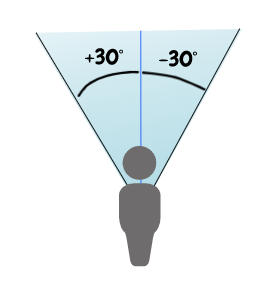
\includegraphics[width=0.3\textwidth]{images/degree_orientation.png}
    \caption{Η κατεύθυνση του χρήστη πρέπει να είναι μέσα σε ένα τόξο 60\degree για να θεωρείται έγκυρη. Αλλιώς παρέχεται κατάλληλη ανάδραση για αριστερή ή δεξιά στροφή.}
    \label{fig:degree-orientation}
\end{figure}
\begin{figure}[H]
    \centering
    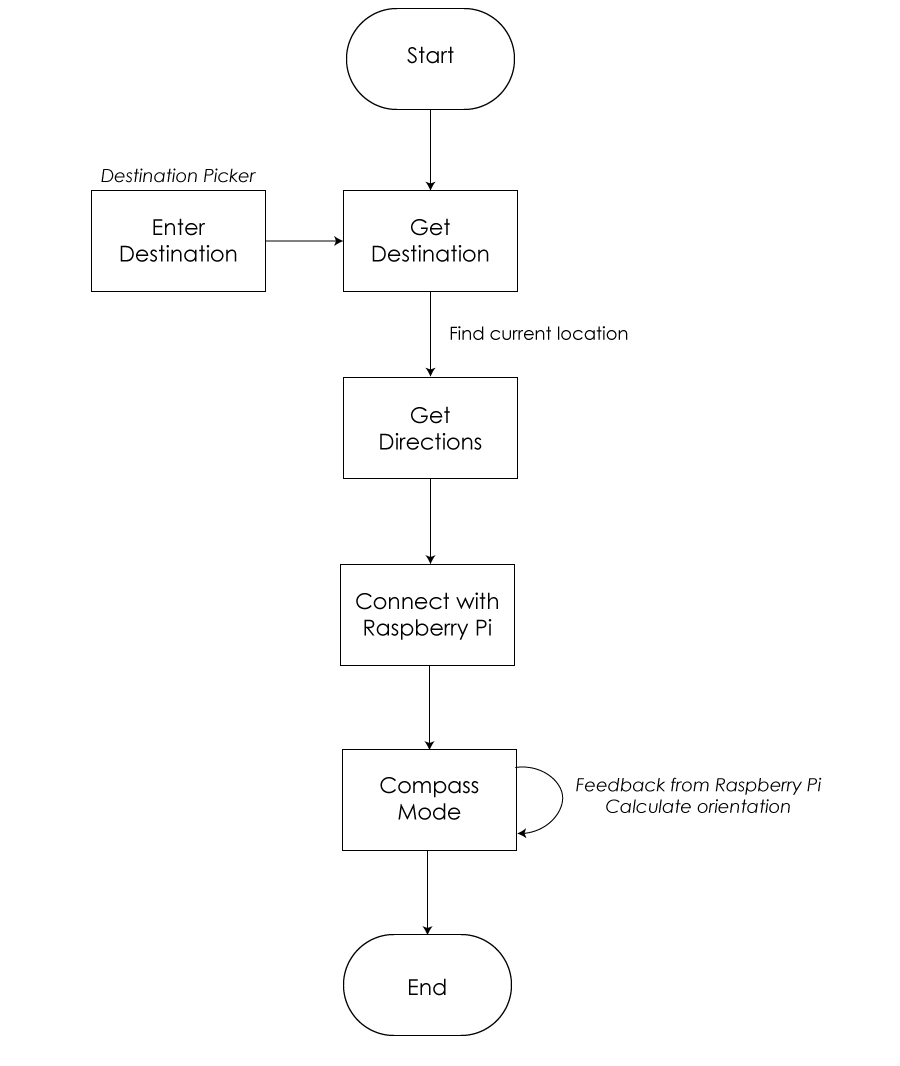
\includegraphics[width=0.8\textwidth]{images/working_diagram.png}
    \caption{Διάγραμμα ροής της Android εφαρμογής}
    \label{fig:working-diagram}
\end{figure}

\subsubsection{Προδιαγραφές εφαρμογής – Ελάχιστες απαιτήσεις}
Κατά την ανάπτυξη της εφαρμογής προέκυψαν διάφορες ανάγκες όσον αφορά την χρήση της από άτομα με προβλήματα όρασης. Βασικός μας στόχος ήταν να είναι όσο πιο απλή γίνεται με έμφαση στη λειτουργικότητα. Μια τέτοια εφαρμογή πρέπει:
\begin{enumerate}
    \item Να χαρακτηρίζεται από την απλότητα στη διεπιφάνεια χρήστη
    \item Να είναι διαισθητική, δηλαδή να είναι αυτονόητο αυτό που προσφέρει μην απαιτείται πολύς χρόνος εκπαίδευσης σε νέους χρήστες
    \item Να χρησιμοποιεί τεχνολογία πρόσβασης για άτομα με μειωμένη όραση, όπως χρήση δονήσεων, μετατροπή λόγου σε κείμενο και αντίστροφα.
\end{enumerate}

Από τις παραπάνω απαιτήσεις, στα πλαίσια της παρούσας εργασίας καταφέραμε να υλοποιήσουμε το 1, 2 και, εν μέρει, το 3. Λόγω περιορισμένου χρόνου δεν υλοποιήθηκε η μετατροπή από προφορικό λόγο σε κείμενο.
\newpage
\subsubsection{UX-UI Design}
Παρακάτω παρουσιάζονται μερικά στιγμιότυπα από τα διάφορα screens της εφαρμογής.
\begin{figure}[H]
    \centering
    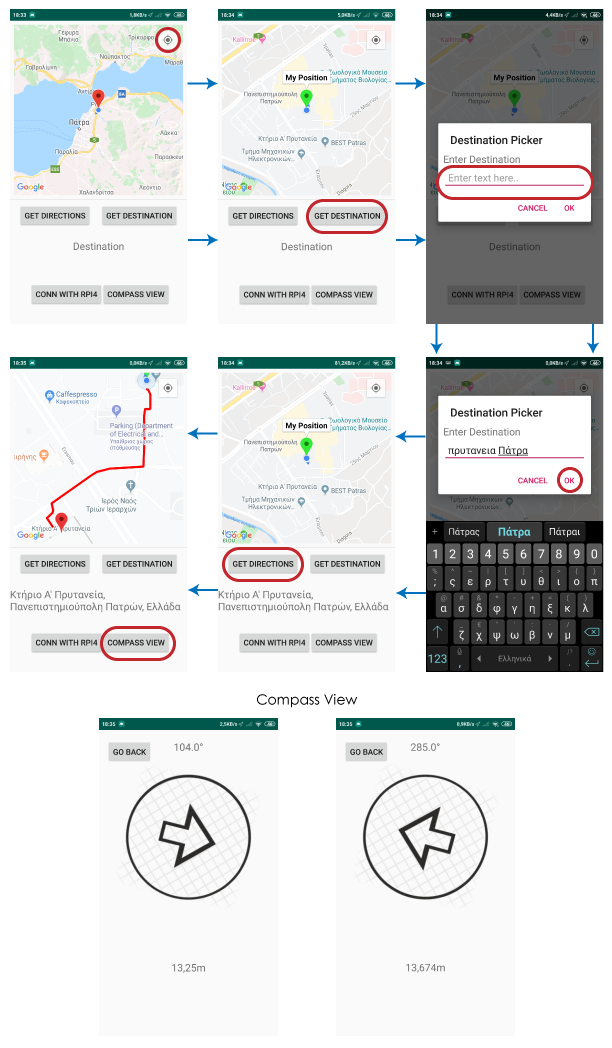
\includegraphics[width=0.7\textwidth]{images/ui_app.png}
    \caption{Διεπιφάνεια επαφής χρήστη}
    \label{fig:ui-app}
\end{figure}

Στο σχήμα \ref{fig:ui-app} παρουσιάζονται με κόκκινο πλαίσιο οι βασικοί τρόποι με τους οποίους αλληλεπιδρά ο χρήστης με το σύστημα. Η βασική ιδέα είναι ότι ο χρήστης, αφού εισάγει τον προορισμό του, θα τοποθετήσει το κινητό στη τσέπη του (ή θα το κρατάει στο χέρι του) και αυτό θα τον καθοδηγεί καθ' όλη την διάρκεια της πλοήγησης, μειώνοντας στο ελάχιστο την αλληλεπίδραση του χρήστη με το σύστημα. Η εφαρμογή εντοπίζει αυτόματα τον προσανατολισμό του χρήστη με τη βοήθεια των αισθητήρων επιταχυνσιομέτρου, γυροσκοπίου και πυξίδας. Είναι γεγονός ότι ο χρήστης που έχει προβλήματα όρασης θα εισάγει τον προορισμό του μέσω ενός συστήματος αναγνώρισης και μετατροπής ομιλίας σε κείμενο. Δυστυχώς, λόγω έλλειψης χρόνου δεν υλοποιήθηκε το συγκεκριμένο χαρακτηριστικό στα πλαίσια της παρούσας διπλωματικής εργασίας.

\subsection{Συσκευή απτικής ανατροφοδότησης – Haptic Device}
\subsubsection{Υπάρχουσες συσκευές απτικής ανατροφοδότησης}
Ως συσκευές απτικής ανατροφοδότησης μπορούν να χαρακτηριστούν όλες εκείνες οι συσκευές που παρέχουν κάποιου είδους πίεση στο δέρμα του χρήστη, π.χ. μέσω δόνησης. Την τελευταία δεκαετία έχουν εμφανιστεί πολλές τέτοιες συσκευές που είναι πολλά υποσχόμενες για την αλληλεπίδραση ανθρώπου-μηχανής. Μια πολύ ενδιαφέρουσα εναλλακτική που εξετάστηκε στα πλαίσια της διπλωματικής είναι το βραχιόλι Myo Armband \cite{MyoGestu49:online}, το οποίο τοποθετείται κάτω από τον αγκώνα και αποτελείται από πολλαπλούς αισθητήρες που διαβάζουν ηλεκτρομυογραφικά σήματα τα οποία ερμηνεύονται ως συγκεκριμένες κινήσεις. Αν και το Myo Armband παρέχει τη δυνατότητα δόνησης στο χέρι του χρήστη, δεν επιλέχθηκε τελικά λόγω του ότι η εταιρεία που το είχε έκλεισε και δεν υπήρχε η απαραίτητη υποστήριξη από την κοινότητα. Επιπλέον, η χρησιμοποίηση της συγκεκριμένης συσκευής θα πρόσθετε ακόμα ένα βάρος στον χρήστη, κάτι που εναντιώνεται στο κριτήριο της απλότητας και της παρεμβατικότητας που αναφέραμε νωρίτερα.

\begin{figure}[H]
    \centering
    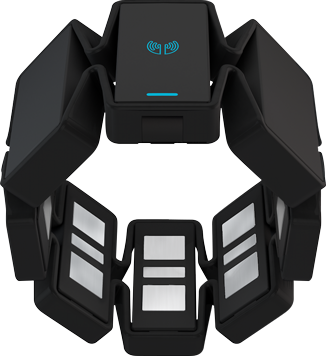
\includegraphics[width=0.6\textwidth]{images/myo_image_black.png}
    \caption{Myo Armband}
    \label{fig:myo}
\end{figure}

\subsubsection{Smartphone}
Μετά από εξέταση όλων των εναλλακτικών, καταλήξαμε στην επιλογή του smartphone ως το μέσο διάδοσης της απτικής ανάδρασης στο χρήστη. Αρχικά, η επιλογή αυτή μας εξυπηρετεί επειδή δεν απαιτείται η ένταξη μιας άλλης συσκευής στο σύστημα, η οποία πιθανόν να είχε προβλήματα συμβατότητας με τα υπόλοιπα μέρη. Επίσης, ο χρήστης δεν επιβαρύνεται με περιττά αντικείμενα, που θα δυσκόλευαν την εξωτερική του μετακίνηση και την εικόνα του προς τον υπόλοιπο κόσμο. Τέλος, το smartphone συνδέεται με το υπόλοιπο σύστημα και λαμβάνει κατάλληλα σήματα σχετικά με τον εντοπισμό και την αναγνώριση διαβάσεων και φαναριών. Ανάλογα το είδος του σήματος που φτάνει στο smartphone, αυτό με τη σειρά του παρέχει το κατάλληλο μοτίβο δόνησης στον χρήστη. Στα πλαίσια της παρούσας διπλωματικής εργασίας χρησιμοποιήθηκε το μοντέλο \emph{Redmi Note 4X}.

\section{Αλγόριθμοι πλοήγησης \& Λογισμικό (Software)}
Στην ενότητα αυτή παρουσιάζονται οι αλγόριθμοι που χρησιμοποιήθηκαν για την υλοποίηση του συστήματος πλοήγησης, καθώς και το λογισμικό που αξιοποιήθηκε για την ανάπτυξή του. Λαμβάνοντας υπόψιν το εύρος της υλοποίησης, ήταν αναγκαίος ο συνδυασμός πολλών διαφορετικών γνώσεων και εργαλείων, γεγονός που πολλές φορές δυσκόλεψε την υλοποίηση λόγω μη συμβατότητας. Παρόλα αυτά, η ενασχόληση του συγγραφέα της εργασίας με τόσα διαφορετικά εργαλεία και γλώσσες προγραμματισμού τον βοήθησε να αποκτήσει μια πιο ολοκληρωμένη άποψη για το συγκεκριμένο ερευνητικό πεδίο και να αναπτύξει πολλές νέες δεξιότητες.

\subsection{Χρησιμοποιηθέντα εργαλεία και γλώσσες προγραμματισμού}
Για την ανάπτυξη της εφαρμογής πλοήγησης σε λειτουργικό Android, επιλέχθηκε το λογισμικό της Google, Android Studio, το οποίο υποστηρίζει συγγραφή κώδικα σε Java, ενώ για την συγγραφή του κώδικα που αφορά τους αλγορίθμους επεξεργασίας εικόνας χρησιμοποιήθηκε το Visual Studio της Microsoft και η συγγραφή έγινε στη γλώσσα C++. Καθ' όλη την υλοποίηση των αλγορίθμων έγινε εκτεταμένη χρήση της γνωστής βιβλιοθήκης OpenCV (Open Computer Vision) και του Intel® RealSense™ SDK (Sofware Development Kit) που παρέχεται από την Intel.

\subsubsection{Android Studio - Java}
Το Android Studio IDE (Intergrated Development Environment) \cite{android_studio:online} είναι ίσως το πιο διαδεδομένο λογισμικό ανάπτυξης εφαρμογών για Android κινητά. Υποστηρίζεται επίσημα από την Google και μπορεί να εγκατασταθεί στις περισσότερες συσκευές (Windows, Mac, Linux). Το λογισμικό αυτό διευκολύνει τον σχεδιασμό του γραφικού περιβάλλοντος της εφαρμογής, δηλαδή της διεπιφάνειας χρήστη, και παρέχει τη δυνατότητα αξιοποίησης όλων των διαθέσιμων υπηρεσιών σε ένα smartphone, π.χ. GPS, IMU sensors, Bluetooth κ.α. Παράλληλα, ένα μεγάλο πλεονέκτημα του Android Studio είναι ότι επιτρέπει το γρήγορο και άμεσο testing της εφαρμογής υπό ανάπτυξη στο κινητό του χρήστη, ή σε κάποιον προσομοιωτή (emulator).

Πιο συγκεκριμένα, χρησιμοποιήθηκε η έκδοση \emph{Android Studio 3.5.1}, η οποία παρέχει την δυνατότητα συγγραφής κώδικα σε Java \cite{wiki:java} και σε Kotlin \cite{wiki:kotlin}, η οποία είναι μια παραλλαγή της Java. Όπως προαναφέρθηκε, επιλέχθηκε η ανάπτυξη σε Java, λόγω της μεγαλύτερης και ευρύτερης υποστήριξης από την κοινότητα.

\begin{figure}[H]
    \centering
    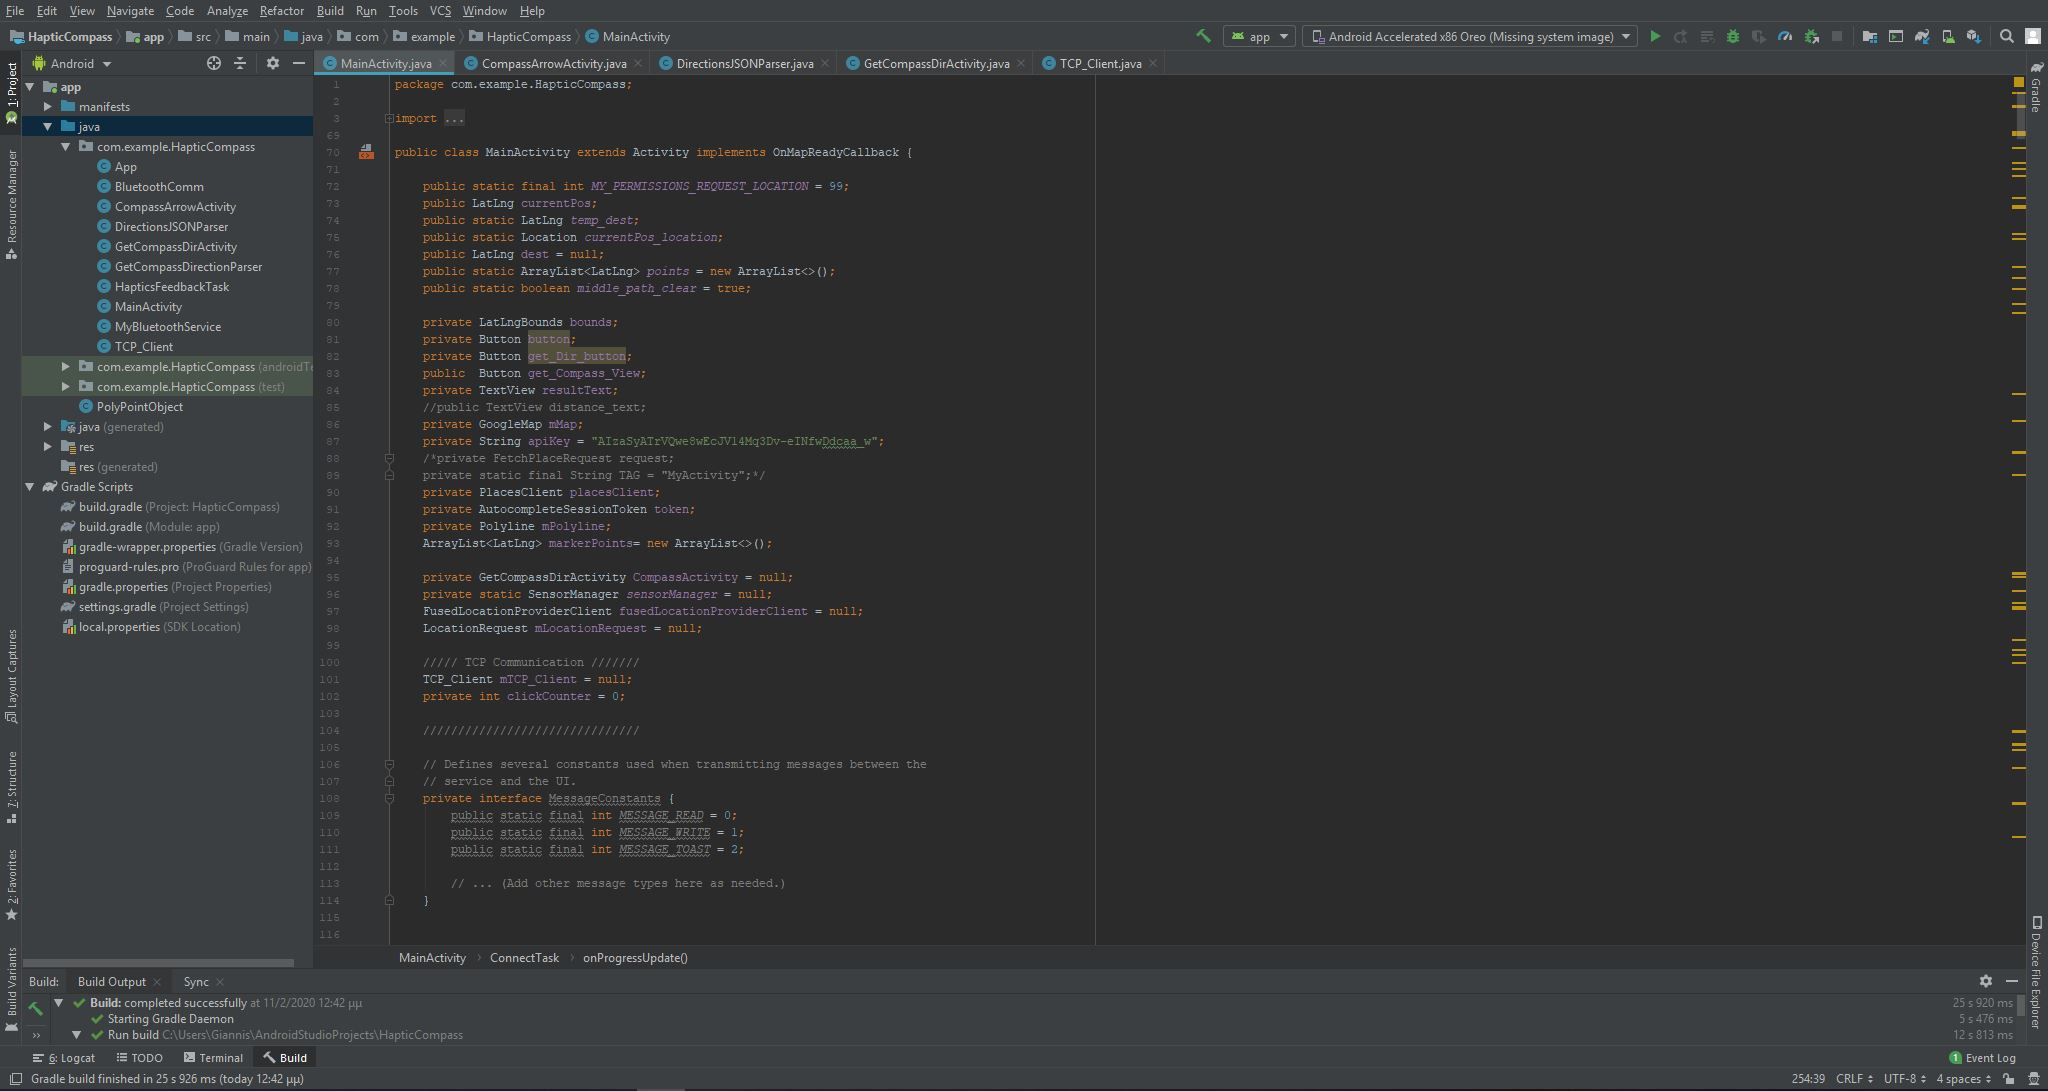
\includegraphics[width=\textwidth]{images/android_studio.JPG}
    \caption{Προγραμματιστικό περιβάλλον Android Studio IDE}
    \label{fig:android-studio}
\end{figure}

\subsubsection{Visual Studio - C++}
Η κύρια ανάπτυξη κώδικα έγινε σε C++ στο περιβάλλον του\emph{ Visual Studio 2017 IDE} \cite{VisualSt72:online}. Πρόκειται για ένα από τα καλύτερα IDE, που προσφέρουν αρκετές διευκολύνσεις κατά την ανάπτυξη κώδικα, όπως είναι η αυτόματη συμπλήρωση, εντοπισμός σφαλμάτων, debugging κ.α. Ένα IDE (Intergrated Development Environment), ή αλλιώς ολοκληρωμένο περιβάλλον ανάπτυξης, είναι μια σουίτα λογισμικού που βοηθάει στην ανάπτυξη προγραμμάτων υπολογιστή και περιλαμβάνει κάποιον επεξεργαστή πηγαίου κώδικα, έναν μεταγλωττιστή, εργαλεία αυτόματης παραγωγής κώδικα, debugger, linker, version control systems (git) και εργαλεία κατασκευής γραφικών διασυνδέσεων χρήστη.

Ως εναλλακτική επιλογή υπήρχε η ανάπτυξη του κώδικα στη γλώσσα Python \cite{wiki:python}, η οποία είναι πολύ διαδεδομένη τα τελευταία χρόνια και υποστηρίζεται σε πολύ μεγάλο βαθμό από την κοινότητα, ωστόσο απορρίφθηκε επειδή στόχος της διπλωματικής ήταν η υλοποίηση κώδικα για embedded συστήματα, όπως το Raspberry Pi, για τα οποία η C++ είναι πιο κατάλληλη γλώσσα. Επίσης, η Python είναι εν γένει πιο αργή σε σύγκριση με την C++, καθώς η πρώτη ακολουθεί μια διαδικασία "μετάφρασης", ενώ η δεύτερη γίνεται compile κατευθείαν σε γλώσσα μηχανής. Τέλος, ο κώδικας που γράφτηκε στο Visual Studio μεταφέρθηκε στο Raspberry Pi αυτούσιος, με μικρές μόνο τροποποιήσεις, ώστε να είναι συμβατός με το λειτουργικό σύστημα Linux του Raspberry Pi.

\begin{figure}[H]
    \centering
    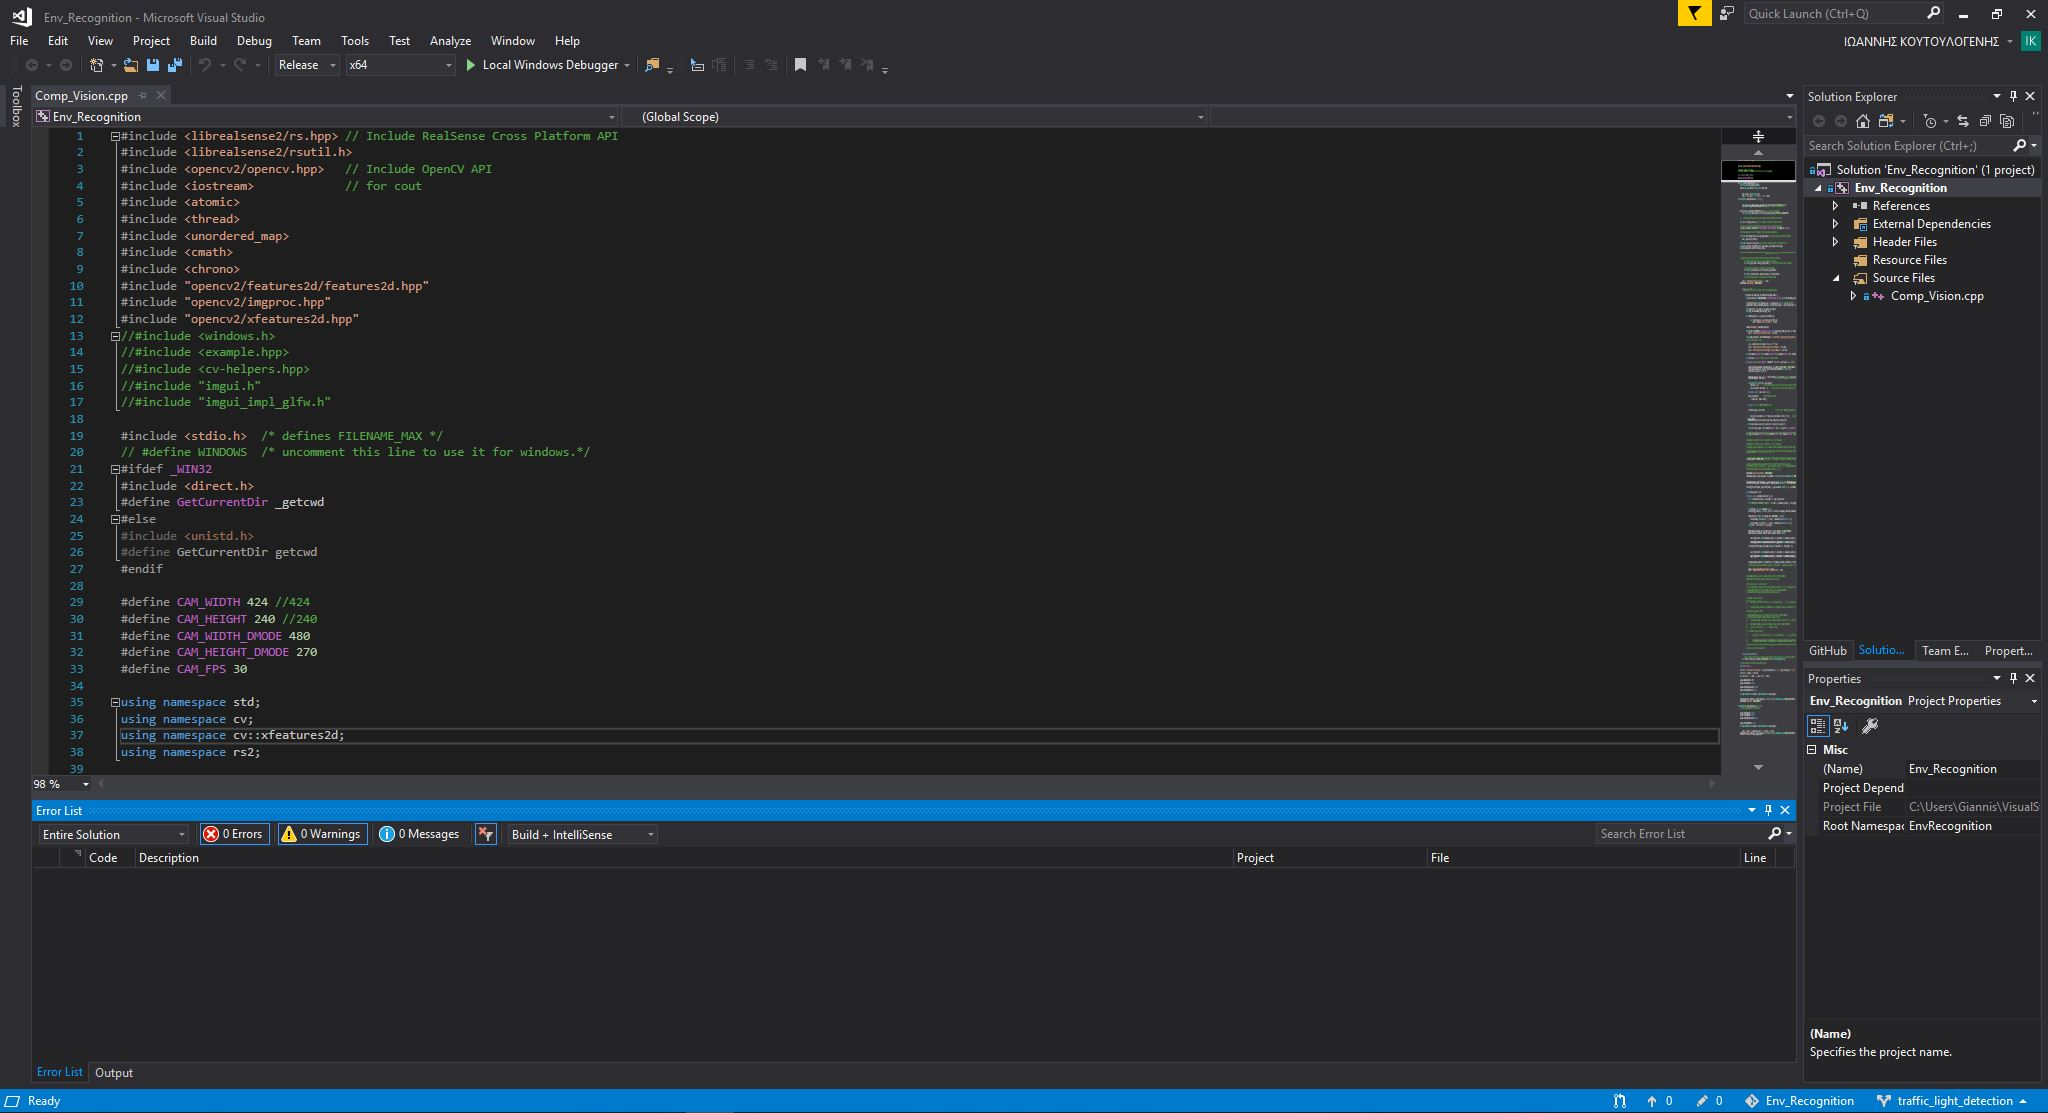
\includegraphics[width=\textwidth]{images/vs17.JPG}
    \caption{Προγραμματιστικό περιβάλλον Visual Studio IDE}
    \label{fig:visual-studio}
\end{figure}

\subsubsection{OpenCV}
Στα πλαίσια της διπλωματικής χρησιμοποιήθηκε η έκδοση \emph{OpenCV 4.2.0}. Η βιβλιοθήκη OpenCV \cite{OpenCVWi26:online} είναι μια συλλογή από βελτιστοποιημένες συναρτήσεις που χρησιμοποιούνται κυρίως στο πεδίο της μηχανικής όρασης, ενώ παράλληλα παρουσιάζει συμβατότητα με τις περισσότερες πλατφόρμες και χρησιμοποιείται κάτω από την άδεια ανοιχτού κώδικα. Ο λόγος που επιλέχθηκε η αξιοποίηση της OpenCV είναι η ενσωμάτωση πολλών έτοιμων φίλτρων και συναρτήσεων για επεξεργασία εικόνας, που είναι ήδη βελτιστοποιημένες για πιο αποδοτική χρήση, επιτρέποντας στον προγραμματιστή να ασχοληθεί με πιο αφηρημένες έννοιες όσον αφορά τον σχεδιασμό του συστήματος. Τέλος, η υποστήριξη της OpenCV από την κοινότητα είναι καθολική και είναι πολύ πιο εύκολο να διορθωθούν τυχόν σφάλματα στον κώδικα. Η κύρια γλώσσα προγραμματισμού καθώς και η γλώσσα στην οποία είναι γραμμένη η OpenCV είναι η C++.

\begin{figure}[H]
    \centering
    
\includegraphics[width=\textwidth]{images/opencv.png}
    \caption{Λογότυπο βιλβιοθήκης OpenCV}
    \label{fig:opencv}
\end{figure}

\subsubsection{Intel® RealSense™ SDK 2.0}
Παράλληλα με την OpenCV αξιοποιήθηκε και η βιβλιοθήκη LibRealsense \cite{IntelRea94:online} που παρέχετε από το SDK της κάμερας Intel Realsense. Πιο συγκεκριμένα, η κάμερα που χρησιμοποιήθηκε έρχεται μαζί με ένα πακέτο συναρτήσεων που υλοποιούν βασικά κομμάτια επικοινωνίας της κάμερας με το πρόγραμμα και διευκολύνουν την πρόσβαση στα δεδομένα της κάμερας, π.χ. depth maps και rgb frames. Παράλληλα, μέσα από το συγκεκριμένο SDK δίνεται η δυνατότητα παρέμβασης στις εσωτερικές προεπιλεγμένες ρυθμίσεις της κάμερας και παρέχονται βασικά παραδείγματα και χρήσιμα εργαλεία αποσφαλμάτωσης (debugging).

\begin{figure}[H]
    \centering
    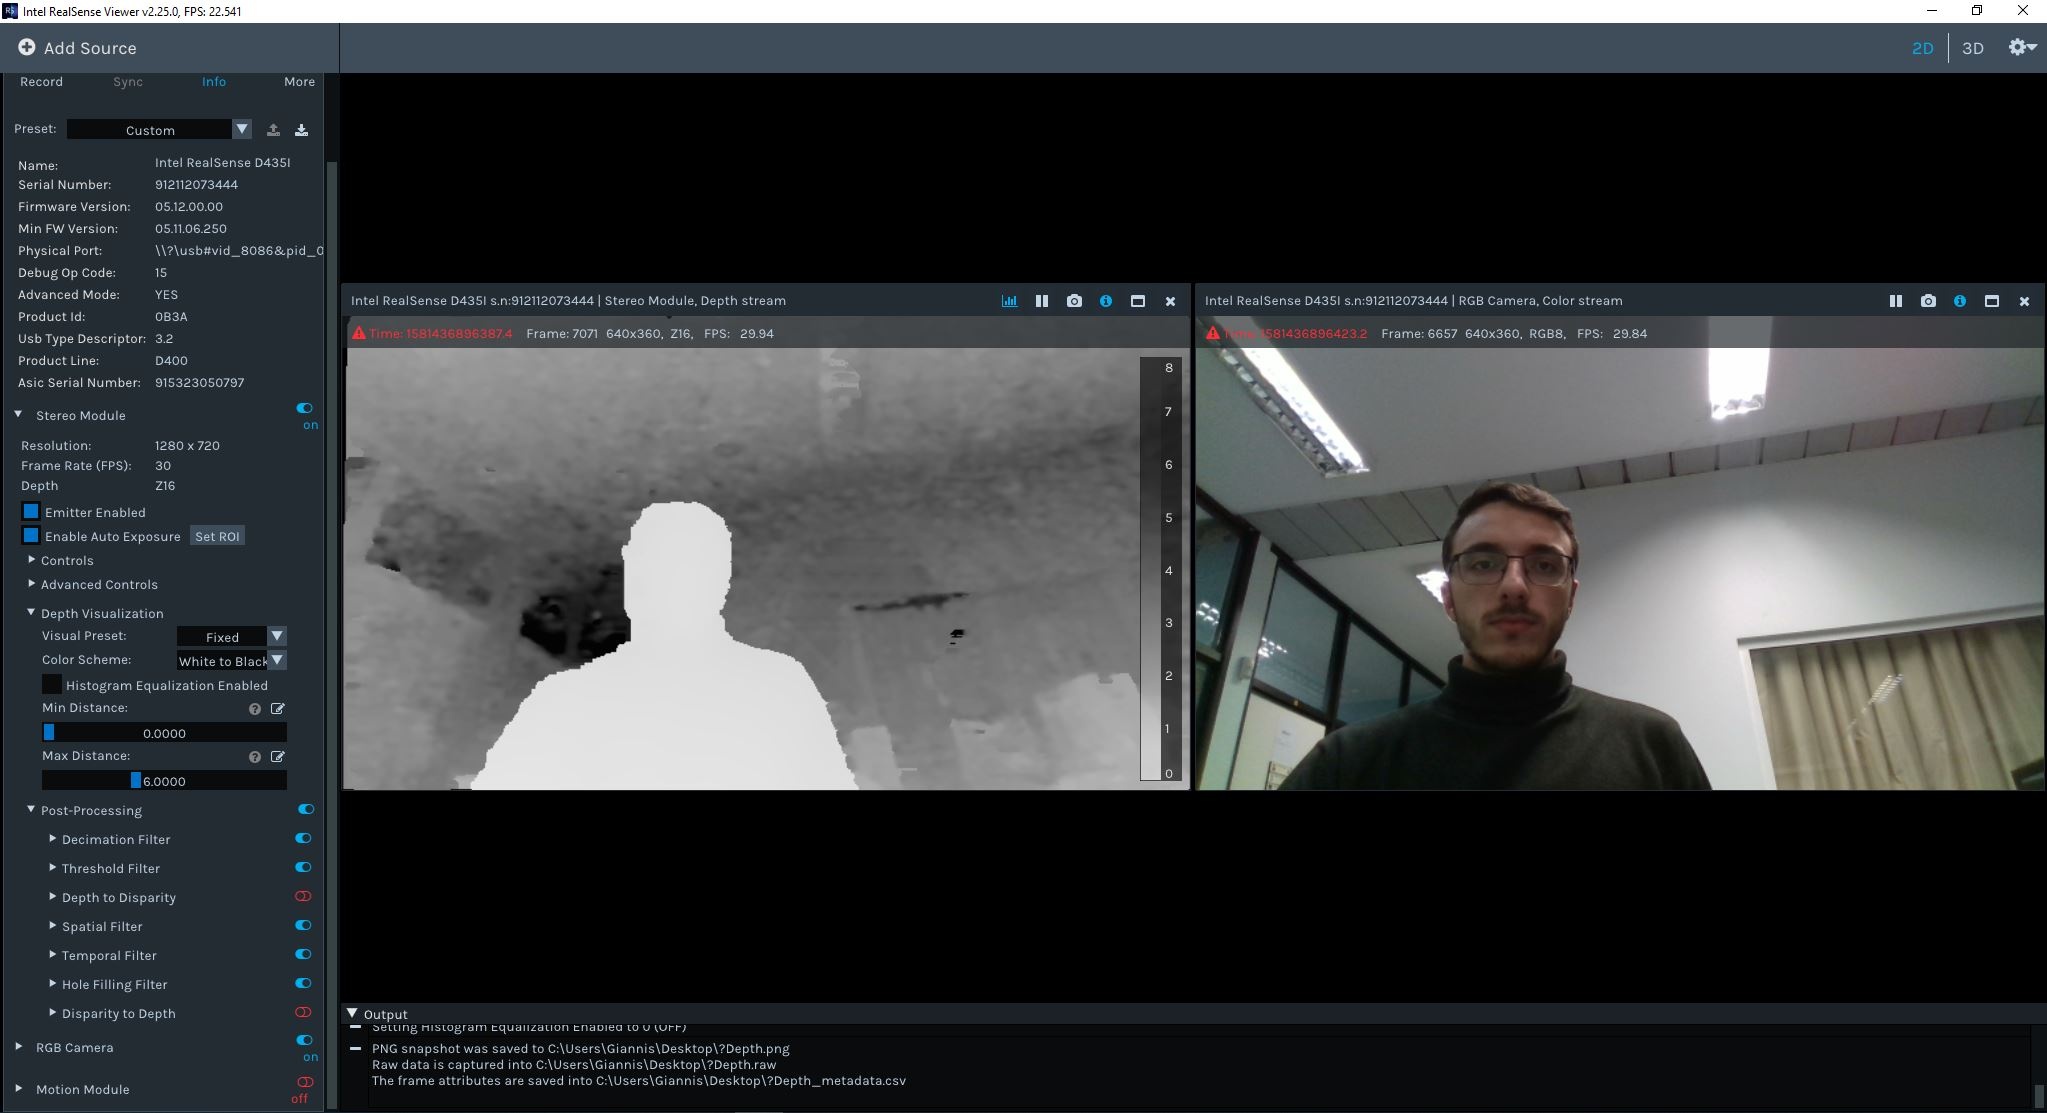
\includegraphics[width=\textwidth]{images/realsense_viewer.JPG}
    \caption{RealSense Viewer από το RealSense™ SDK 2.0}
    \label{fig:librealsense}
\end{figure}

\subsubsection{Raspberry Pi - Linux OS}
Το λειτουργικό που χρησιμοποιήθηκε στο Raspberry Pi 4 είναι το \emph{Ubuntu Server 19.10} 64-bit \cite{InstallU96:online}, με κωδική ονομασία Eoan Ermine, το οποίο υποστηρίζει πλήρως τις δυνατότητες του RPi4. Επειδή το λειτουργικό σύστημα Ubuntu Server δεν έχει ενσωματωμένο γραφικό περιβάλλον, εγκαταστάθηκε το MATE Desktop Environment \cite{MATEDesk37:online}.

\begin{figure}[H]
    \centering
    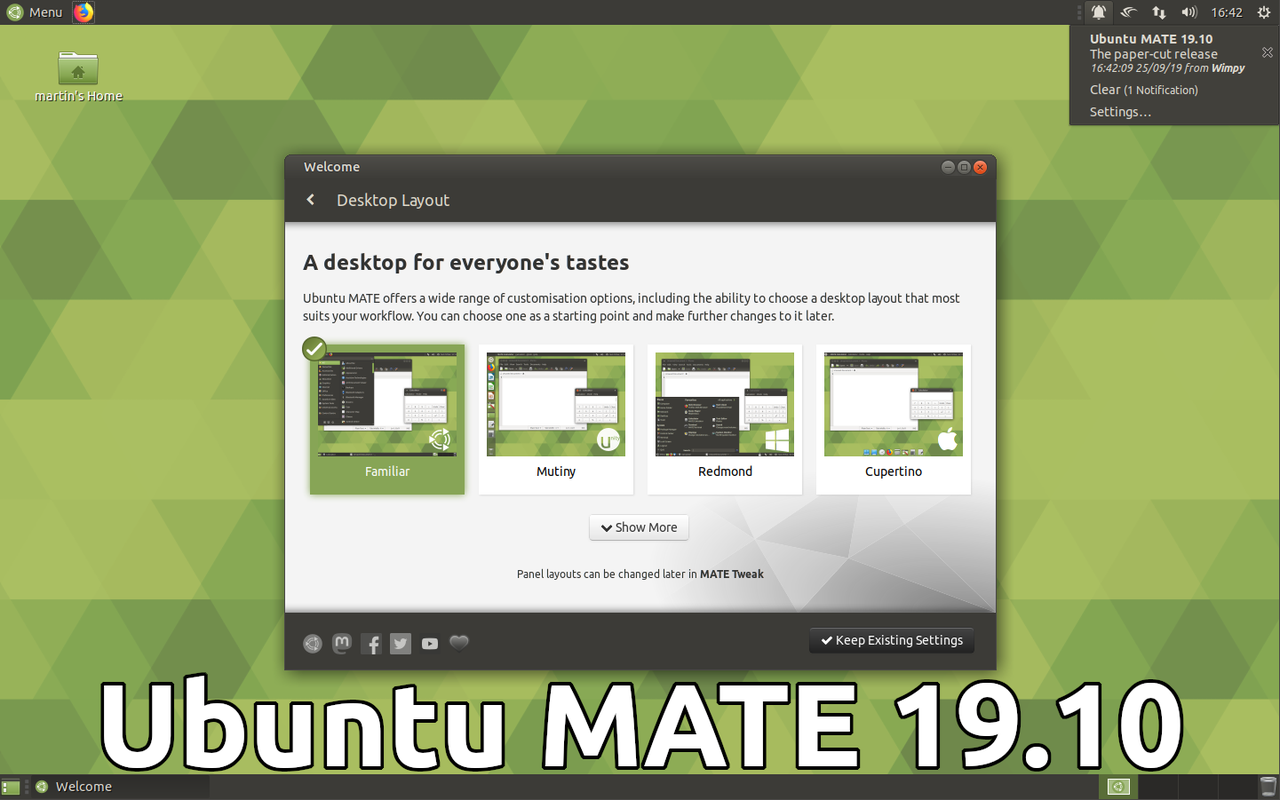
\includegraphics[width=\textwidth]{images/eoan-ermine-desktop.png}
    \caption{Ubuntu 19.10 with MATE Desktop Environment}
    \label{fig:mate}
\end{figure}

\subsection{Αλγόριθμοι επεξεργασίας εικόνας σε πραγματικό χρόνο}
Παρακάτω αναλύονται οι αλγόριθμοι που χρησιμοποιήθηκαν στην παρούσα διπλωματική εργασία, αποφεύγοντας όσο γίνεται τις πολύ τεχνικές λεπτομέρειες που αφορούν την προγραμματιστική υλοποίησή τους. Αρχικά, είναι σημαντικό να αναφέρουμε ότι το πρόγραμμά μας αποτελείται από δύο διαφορετικά threads, δηλαδή κομμάτια κώδικα που τρέχουν το ένα ανεξάρτητα από το άλλο, όπου το πρώτο thread (εφεξής \emph{processing thread}) τρέχει στο παρασκήνιο και είναι υπεύθυνο για να "παραλαμβάνει" τα frames από την κάμερα και να εφαρμόζει ένα αρχικό φιλτράρισμα μόνο στα depth frames, ενώ στο δεύτερο thread (εφεξής \emph{main thread}) γίνεται η κυρίως επεξεργασία και ανάλυση των εικόνων και τρέχει σε ένα συνεχή βρόχο για όσο είναι ανοιχτό το πρόγραμμα. Ο λόγος που χρησιμοποιούμε δύο διαφορετικά thread είναι για να αποφύγουμε καταστάσεις όπου το πρόγραμμα "κολλάει" αναμένοντας κάποιο frame να φτάσει από την κάμερα.

\begin{figure}[H]
    \centering
    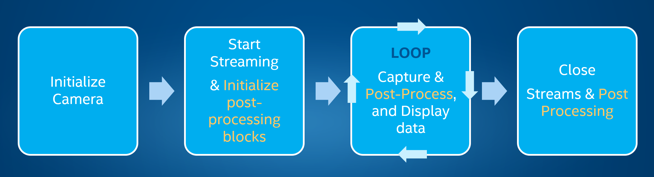
\includegraphics[width=0.8\textwidth]{images/frames_flow.png}
    \caption{Διάγραμμα ροής ενός frame}
    \label{fig:frame-flow}
\end{figure}

Το πρόγραμμα ρυθμίζεται να λειτουργεί με RGB frames ανάλυσης 424x240 στα 30fps και Depth frames ανάλυσης 480x270 στα 30fps. Οι συγκεκριμένες αναλύσεις επιλέχθηκαν ώστε να κάνει την επεξεργασία πιο γρήγορη, μιας και δεν είναι αναγκαία μεγαλύτερη ενάλυση για την εφαρμογή που θέλουμε. Στη συνέχεια, αφού παραληφθεί κάποιο depth frame στο processing thread, εφαρμόζονται τα εξής φίλτρα με σειρά προτεραιότητας \cite{DepthPos51:online}:
\begin{enumerate}
    \item \textbf{Decimation filter}: Φίλτρο που μειώνει την πολυπλοκότητα της εικόνας, εφαρμόζοντας ουσιαστικά υπο-δειγματοληψία (downsampling) της αρχικής εικόνας. Πιο συγκεκριμένα, εφαρμόζεται συνέλιξη του αρχικού frame με ένα πίνακα kernel 2x2, χρησιμοποιώντας την μέση τιμή των pixel που καλύπτονται από τον kernel. Αντίστοιχα, το μέγεθος της εικόνας μειώνεται αναλογικά και στις δύο διαστάσεις για να διατηρηθεί η αρχική αναλογία διαστάσεων. Η διαδικασία αυτή μπορεί να αυξήσει την ταχύτητα της μετέπειτα επεξεργασίας μέχρι 4 φορές, ενώ παράλληλα συμβάλλει στην εξάλειψη τυχόν κενών pixels (black holes).
    \item \textbf{Spatial Edge-Preserving filter}: Φίλτρο που εξομαλύνει τον θόρυβο βάθους (depth noise), διατηρεί τις γωνίες/άκρες και κάνει τις επιφάνειες πιο επίπεδες \cite{GastalOliveira2011DomainTransform}.
    \begin{figure}[H]
        \centering
        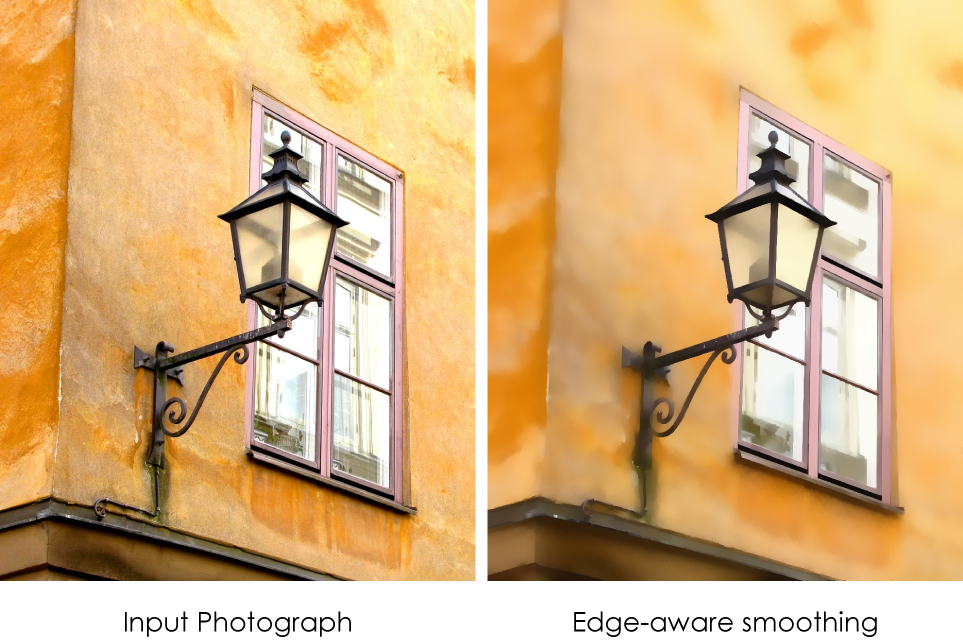
\includegraphics[width=0.8\textwidth]{images/edge_preserving_example.png}
        \caption{Παράδειγμα εφαρμογής του Spatial Filter βασιζόμενο στο \cite{GastalOliveira2011DomainTransform}}
        \label{fig:spatial-example}
    \end{figure}

    \item \textbf{Temporal filter}: Φίλτρο που βελτιώνει τα δεδομένα βάθους με βάση τα αντίστοιχα frames σε προηγούμενη χρονική περίοδο. Πιο συγκεκριμένα, για κάθε pixel που είναι κενό ή έχει λανθασμένη τιμή κοιτάζει το ιστορικό και χρησιμοποιεί την τιμή που είχε το pixel αυτό σε προηγούμενο frame. Ο κανόνας που χρησιμοποιείται είναι ότι η τιμή ενός κενού pixel αντικαθίσταται από την τελευταία έγκυρη τιμή, αν αυτή είναι έγκυρη στα τελευταία 2 από τα 4 frames.
    \item \textbf{Hole-Filling filter}: Φίλτρο που χρησιμοποιείται για εξάλειψη τυχόν εναπομείναντων κενών pixels (holes). Το φίλτρο κάνει αναζήτηση σε μια γειτονιά ενός pixel και η διαδικασία που ακολουθείται είναι ότι κάθε κενό pixel αντικαθίσταται από την τιμή του γειτονικού pixel με την κοντινότερη απόσταση από τον αισθητήρα (nearest from around).
    \begin{figure}[H]
        \centering
        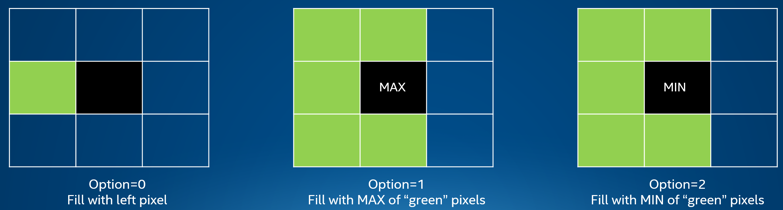
\includegraphics[width=0.8\textwidth]{images/hole_filling.png}
        \caption{Επιλογές φίλτρου εξάλειψης κενών pixels (hole filling)}
        \label{fig:hole-filling}
    \end{figure}
\end{enumerate}

Στη συνέχεια, τα RGB και Depth frames προωθούνται στο main thread και ξεκινάει η εφαρμογή των αλγορίθμων που θα περιγραφεί παρακάτω.

\begin{figure}[H]
    \centering
    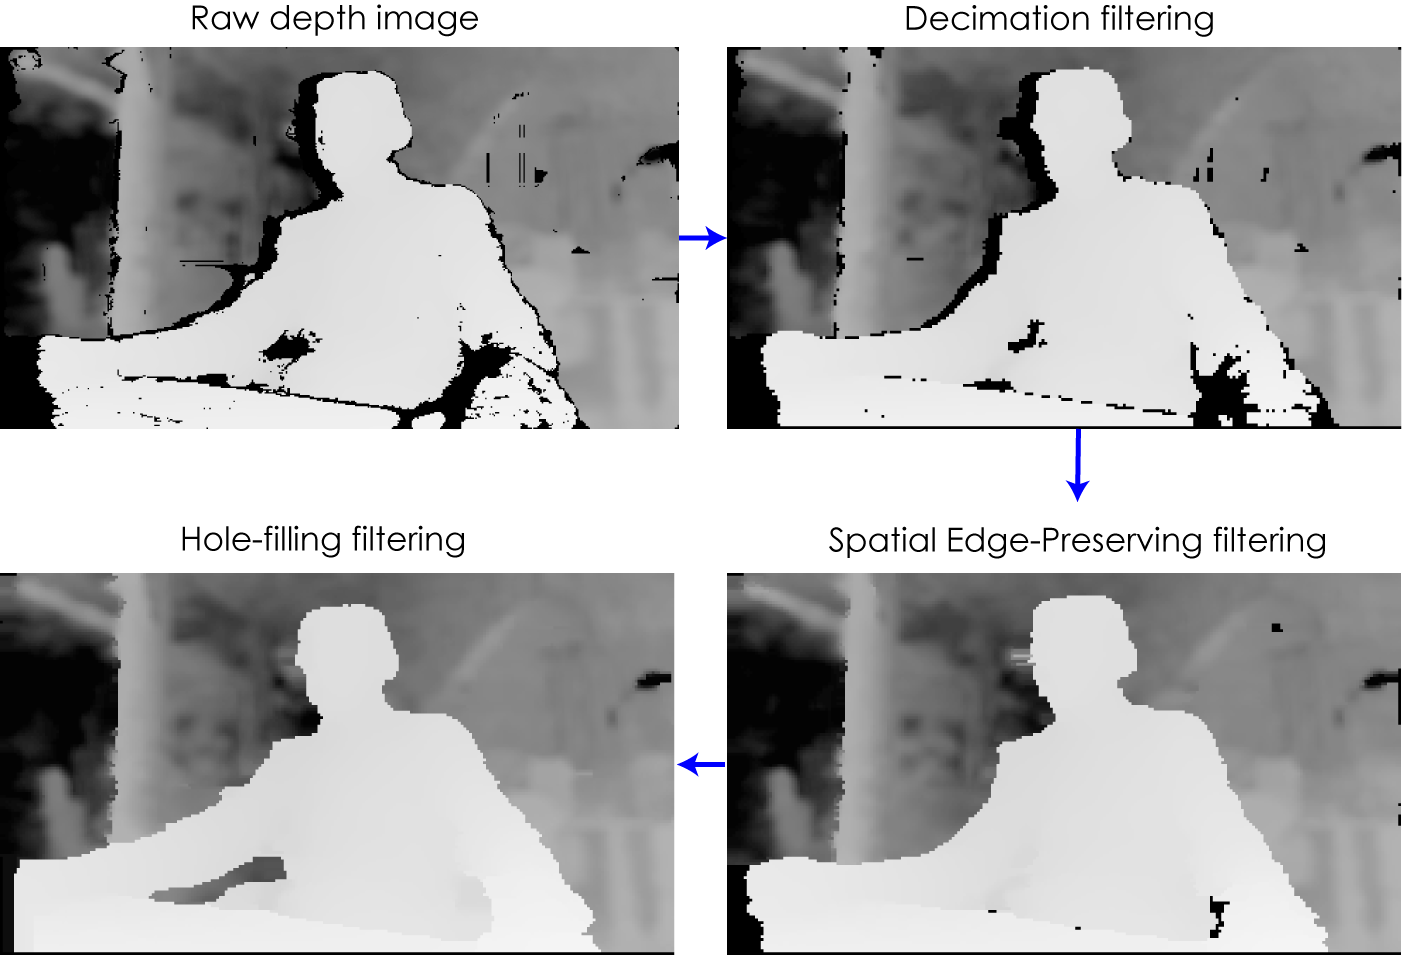
\includegraphics[width=0.8\textwidth]{images/preprocessing.png}
    \caption{Παράδειγμα εφαρμογής φίλτρων στο στάδιο του preprocessing (εξαιρείται το temporal filter, γιατί στην συγκεκριμένη λήψη δεν άλλαζε σημαντικά το αποτέλεσμα)}
    \label{fig:preprocessing}
\end{figure}

\subsubsection{Αναγνώριση διάβασης πεζών}
Η αναγνώριση διάβασης πεζών βασίζεται σε μια παραλλαγή του αλγορίθμου που προτείνεται από τους Wu, X., Hu, R., \& Bao, Y. (2019), στη δημοσίευση με τίτλο \emph{Block-Based Hough Transform for Recognition of Zebra Crossing in Natural Scene Images} \cite{wu_block-based_2019}. Βασική προϋπόθεση είναι να τρέχει σε πραγματικό χρόνο (real-time) και να παρέχει αξιόπιστα αποτελέσματα. Ο προτεινόμενος αλγόριθμος βασίζεται στην εφαρμογή του Μετασχηματισμού Hough σε συγκεκριμένα τμήματα της αρχικής εικόνας που καλούνται blocks και χωρίζεται σε δύο φάσεις:
\begin{enumerate}
    \item την φάση της αναγνώρισης ανά block (\nameref{block-based}), και
    \item την φάση της σύνθεσης (\nameref{synthesize}). 
\end{enumerate}

\paragraph{Χαρακτηριστικά και περιορισμοί διάβασης πεζών}
Η κλασσική διάβαση πεζών αποτελείται από λευκές και μαύρες λωρίδες που εναλλάσσονται μεταξύ τους και θυμίζουν το ασπρόμαυρο μοτίβο της ζέβρας (Σχήμα \ref{fig:zebra-crossing}). Το σύστημα πλοήγησης που παρουσιάζεται στη συγκεκριμένη εργασία θέτει ως βασική προϋπόθεση την ύπαρξη διάβασης πεζών τύπου ζέβρας, ώστε να μπορεί να βοηθήσει τον χρήστη να διασχίσει ένα δρόμο. Τέτοιου τύπου διαβάσεις χαρακτηρίζονται από τις 2 παρακάτω ιδιότητες:
\begin{itemize}
    \item Οι μεγάλες πλευρές των λωρίδων είναι παράλληλες
    \item Η χρωματική ένταση έχει διπολικά χαρακτηριστικά (άσπρο-μαύρο)
\end{itemize}
Ωστόσο, πολλές φορές οι παραπάνω ιδιότητες εκφυλίζονται όταν πρόκειται για διαβάσεις στο πραγματικό περιβάλλον, επειδή άλλοι παράγοντες (όπως συνθήκες φωτισμού, αντανακλάσεις, ξεθώριασμα, γεωμετρία δρόμου, οπτική παρεμπόδιση) επηρεάζουν σημαντικά το πως φαίνονται οι διαβάσεις.

\begin{figure}[H]
    \centering
    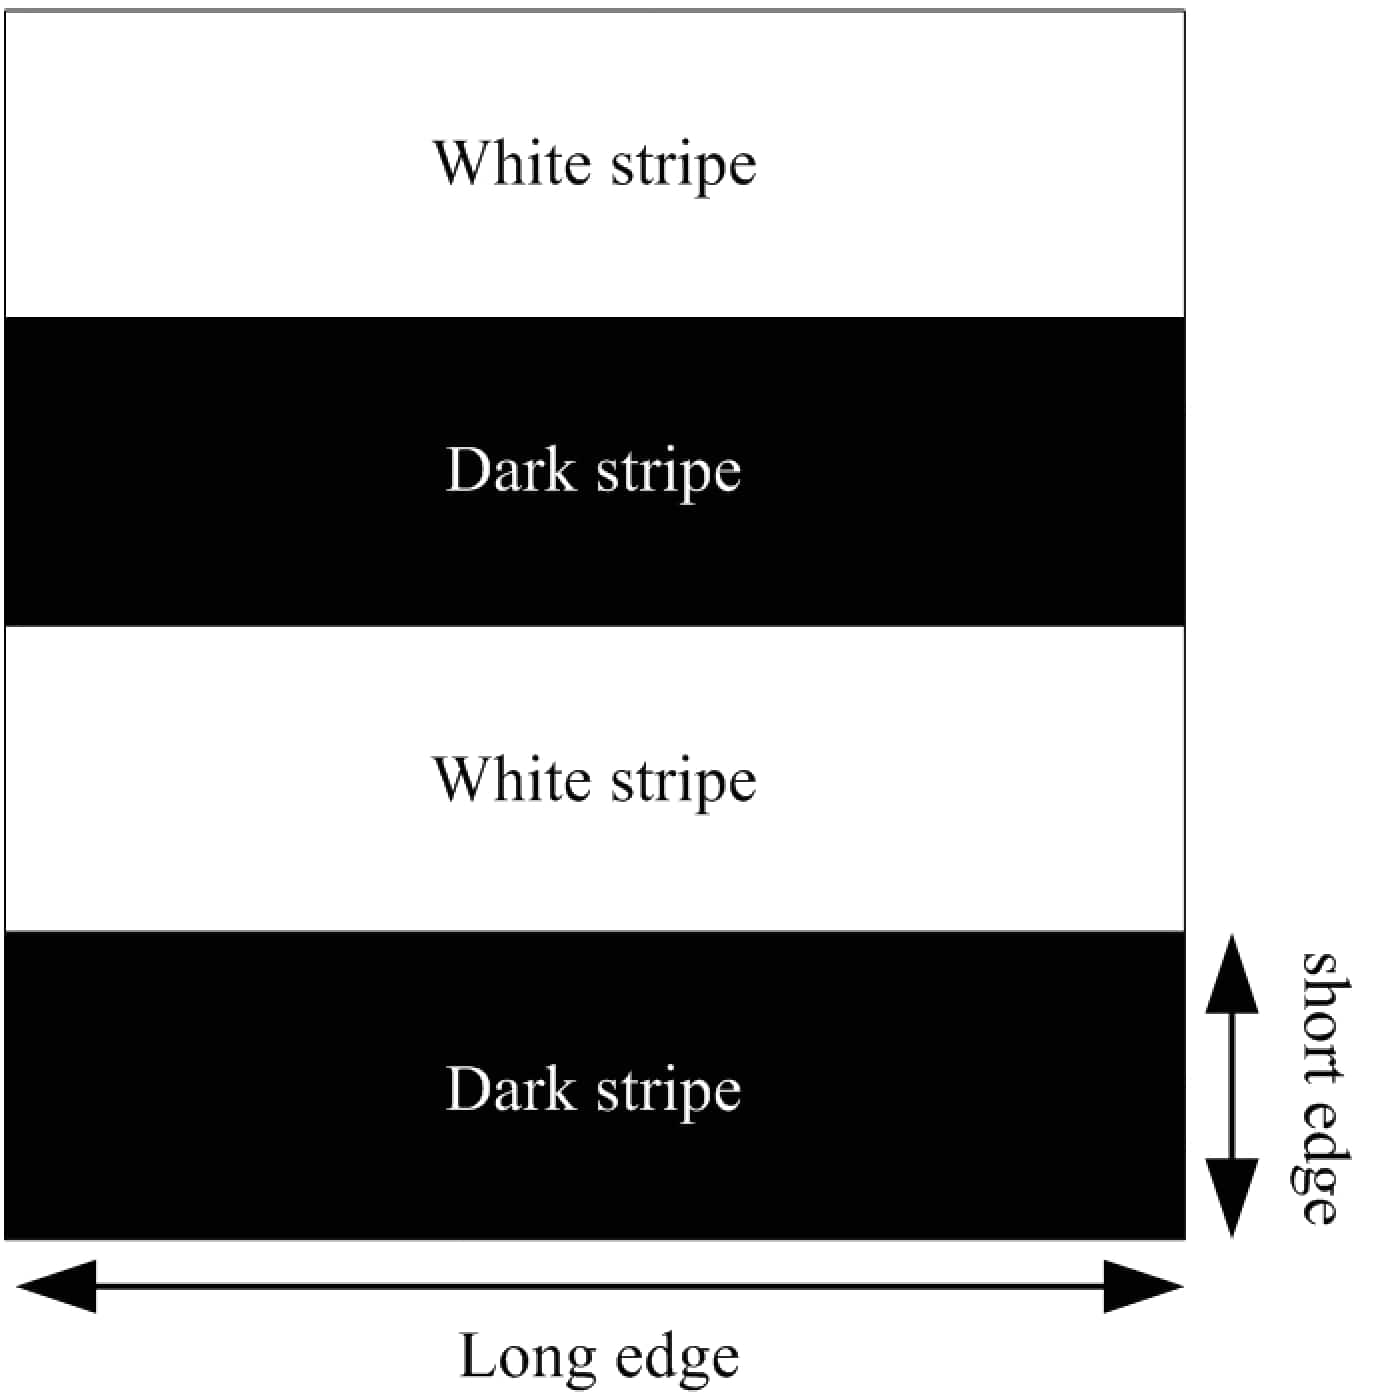
\includegraphics[width=0.5\textwidth]{images/zebra_crossing.jpg}
    \caption{Κλασσική μορφή διάβασης πεζών τύπου ζέβρας \cite{wu_block-based_2019}}
    \label{fig:zebra-crossing}
\end{figure}

\paragraph{Η προτεινόμενη μέθοδος}
Επειδή συνήθως οι διαβάσεις πεζών βρίσκονται στο κάτω μέρος της εικόνας όπως στέκεται ένας πεζός, καταρχήν περιορίζουμε την αρχική εικόνα ορίζοντας μια περιοχή ενδιαφέροντος, η οποία περιλαμβάνει το κάτω μισό της αρχικής εικόνας (50\% του ύψους) και το 80\% του αρχικού πλάτους. Έπειτα αυτή η περιοχή διαιρείται σε πολλαπλά επικαλυπτόμενα blocks που έχουν ίδιο ύψος με την περιοχή ενδιαφέροντος, αλλά μικρότερο πλάτος. Αφού οριστεί το μέγεθος κάθε block (στη παρούσα εργασία επιλέχθηκε το πλάτος κάθε block ίσο με το 1/3 του πλάτους της περιοχής ενδιαφέροντος), το πρόγραμμα μπαίνει σε έναν βρόχο όπου εφαρμόζεται ο Μετασχηματισμός Hough σε κάθε επιμέρους block. Όπως αναφέρθηκε, τα blocks είναι επικαλυπτόμενα, δηλαδή σε κάθε επανάληψη του βρόχου μπαίνει ένα νέο block το οποίο είναι μετατοπισμένο κατά μερικά pixels πιο δεξιά στον άξονα x σε σχέση με το προηγούμενο, μέχρι να φτάσουμε στο τέλος της περιοχής ενδιαφέροντος.
\begin{displayquote}
\emph{Ο αριθμός των pixels που μετατοπίζεται το block σε κάθε επανάληψη εξαρτάται από την επιλογή του χρήστη και επηρεάζει άμεσα την ποιότητα αλλά και την ταχύτητα του αλγορίθμου.}
\end{displayquote}
Όσο μικρότερη είναι η μετατόπιση του block τόσο πιο αναλυτικός γίνεται ο αλγόριθμος και παράγει καλύτερα αποτελέσματα, σε βάρος όμως της ταχύτητας. Αντίθετα, όσο μεγαλύτερη γίνεται η μετατόπιση τόσο πιο γρήγορος γίνεται ο αλγόριθμος με αντίστοιχη μείωση της ποιότητας του αποτελέσματος. Στη παρούσα εργασία, μετά από αρκετές δοκιμές, επιλέχθηκε εμπειρικά η μετατόπιση κατά 75 pixels σε κάθε επανάληψη, που αποτελεί έναν "καλό" συμβιβασμό ανάμεσα στην ποιότητα και την ταχύτητα.

Ο αλγόριθμος χρησιμοποιεί μια λογική όπου σε κάθε pixel ανατίθεται ένα σκορ, το οποίο στην αρχή είναι μηδέν. Εάν εντοπιστούν παράλληλες γραμμές σε ένα block, τότε εκτιμάται η γωνία τους και μεταβάλεται το σκορ των pixels που περιέχονται σε αυτό το block κατά μία συγκεκριμένη φόρμουλα που παρουσιάζεται παρακάτω:$$score[pixel] = 0.2\times score[pixel] + 0.8\times number\textunderscore of\textunderscore pixels\textunderscore in\textunderscore parallel\textunderscore lines$$ Παρατηρούμε ότι το σκορ ενός pixel του block εξαρτάται κατά 20\% από την προηγούμενη τιμή του και κατά 80\% από το πόσο ισχυρή είναι η παρουσία των παράλληλων γραμμών στο εκάστοτε block. Αφού η διαδικασία αυτή γίνει για κάθε block, στο τέλος υπολογίζεται ο μέσος όρος των γωνιών, ώστε να βρεθεί η κατεύθυνση της διάβασης, και τα αθροιστικά σκορ συνθέτονται για να βρεθεί η θέση της διάβασης στην εικόνα.

\begin{figure}[H]
    \centering
    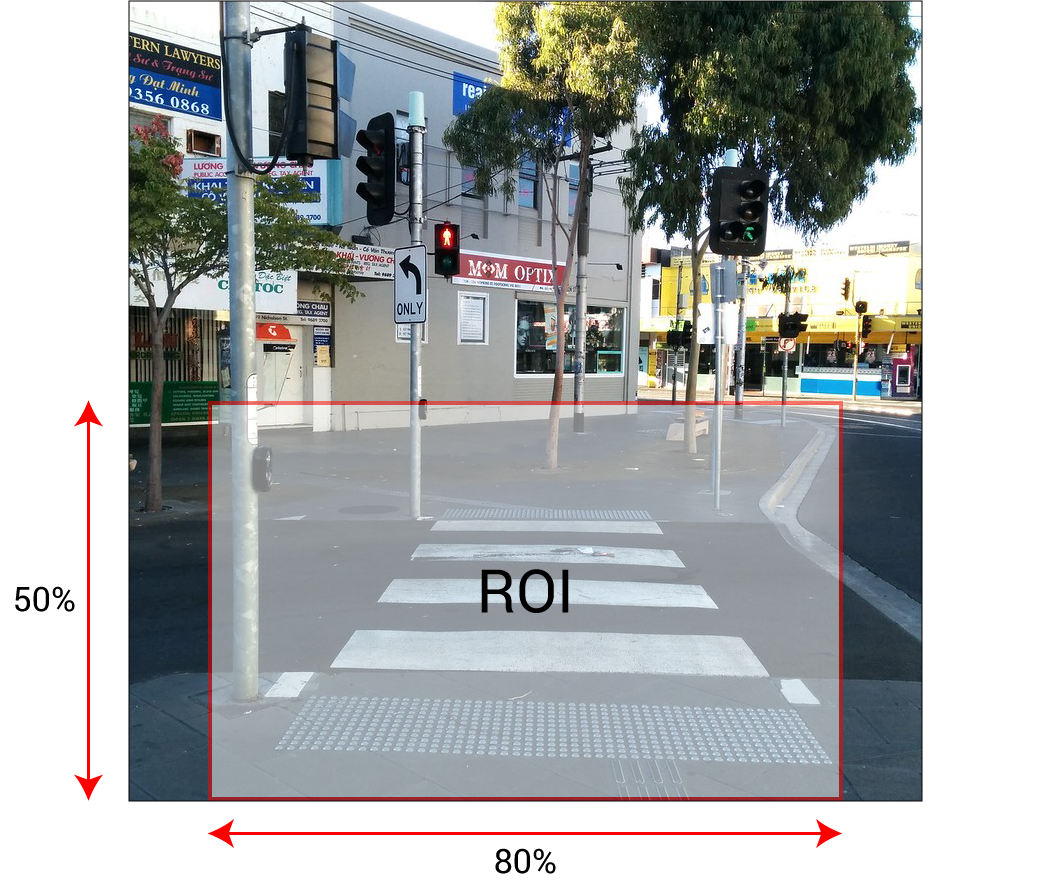
\includegraphics[width=0.6\textwidth]{images/lower_roi.png}
    \caption{Επιλογή περιοχής ενδιαφέροντος (ROI) για εντοπισμό διάβασης πεζών}
    \label{fig:lower-roi}
\end{figure}

\paragraph{Canny Edge Detector \& Hough Transform}
Στην υλοποίηση χρησιμοποιήθηκαν δύο πολύ διαδεδομένες τεχνικές στο χώρο της επεξεργασίας εικόνας, ο μετασχηματισμός Hough και το φίλτρο Canny:
\begin{itemize}
    \item \emph{Canny Edge Detector}: Το φίλτρο Canny αποτελεί μια από τις πιο γνωστές μεθόδους εξαγωγής των ακμών από μια εικόνα \cite{wiki:canny}. Ως ακμή ορίζεται το όριο μεταξύ περιοχών με σχετικά διακριτές τιμές χρωματικών πυκνοτήτων. Με τον όρο ακμές για μια ασπρόμαυρη εικόνα, αναφερόμαστε σε αλλαγές της φωτεινότητας μεταξύ γειτονικών περιοχών της. Τα βήματα του φίλτρου Canny είναι τα ακόλουθα:
    \begin{itemize}
        \item Βήμα 1: Εφαρμογή του γκαουσιανού φίλτρου (Gaussian Filtering) για εξομάλυνση της εικόνας και ελαχιστοποίηση της επίδρασης του θορύβου.
        \begin{figure}[H]
            \centering
            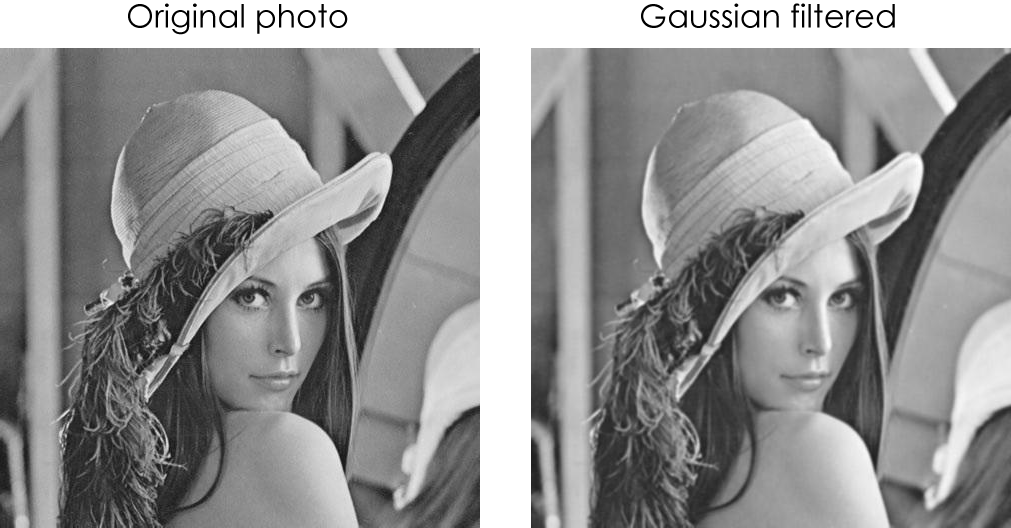
\includegraphics[width=0.8\textwidth]{images/gaussian_filtr.png}
            \caption{Εφαρμογή Gaussian Filter}
            \label{fig:gaussian}
        \end{figure}
        \item Βήμα 2: Εφαρμογή του τελεστή διαφόρισης στην εικόνα (συνέλιξη τελεστή με εικόνα Α) για να βρεθεί η κατευθυντική παράγωγος της εικόνας. Το φίλτρο Canny που υλοποιείται στην βιβλιοθήκη OpenCV χρησιμοποιεί τον τελεστή Sobel \cite{wiki:sobel}:
        \[ G_x = \begin{bmatrix}
            +1 & 0 & -1\\
            +2 & 0 & -2\\
            +1 & 0 & -1\\
        \end{bmatrix} * A, G_y = \begin{bmatrix}
            +1 & +2 & +1\\
            0 & 0 & 0\\
            -1 & -2 & -1\\
        \end{bmatrix} * A \]
        Το μέτρο της παραγώγου δίνεται από την $G = \sqrt{G_x^2 + G_y^2}$ και η κατεύθυνση από την $\Theta = \arctan(\frac{G_y}{G_x})$.
        \begin{figure}[H]
            \centering
            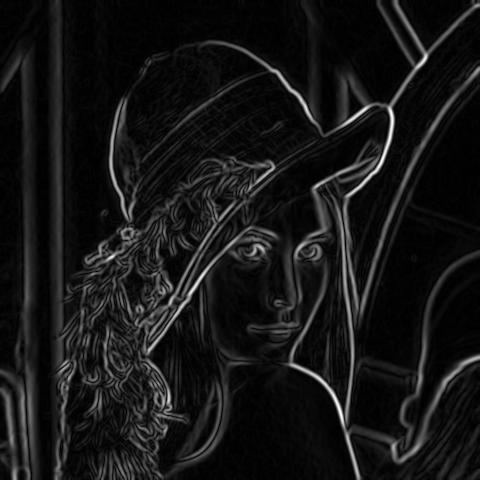
\includegraphics[width=0.5\textwidth]{images/gmag.jpg}
            \caption{Εφαρμογή τελεστή Sobel για εύρεση κατευθυντικών παραγώγων}
            \label{fig:gmag}
        \end{figure}
        \item Βήμα 3: Non Maximum Suppresion (απαλοιφή των μη-µεγίστων) για την διατήρηση μόνο των έντονων ακμών.
        \begin{figure}[H]
            \centering
            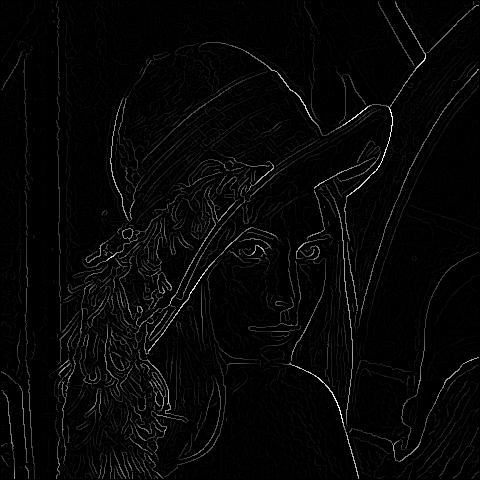
\includegraphics[width=0.5\textwidth]{images/non_maximum_suppression.jpg}
            \caption{Εφαρμογή Non Maximum Suppresion}
            \label{fig:non-maxima}
        \end{figure}
        \item Βήμα 4: Εφαρμογή κατωφλίωσης (double thresholding) για τον περαιτέρω διαχωρισμό των αχνών ακμών.
        \begin{figure}[H]
            \centering
            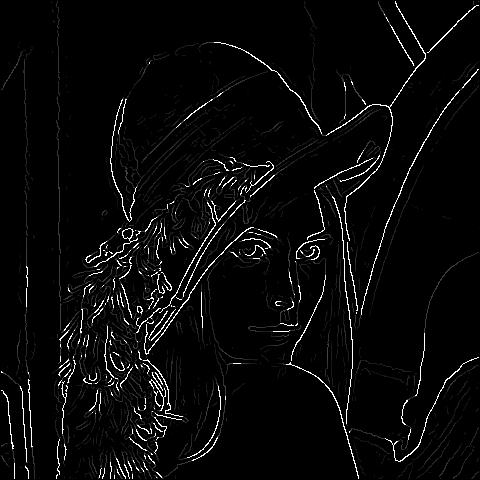
\includegraphics[width=0.5\textwidth]{images/double_threshold.jpg}
            \caption{Εφαρμογή Double Thresholding}
            \label{fig:double-thresholding}
        \end{figure}
        \item Βήμα 5: Αφού έχουμε διαχωρίσει τις έντονες από τις αχνές ακμές, εφαρμόζουμε κατωφλίωση των ακμών με υστέρηση, δηλαδή διατήρηση μόνο των έντονων ακμών και των αχνών ακμών που συνδέονται με έντονες. Αυτό παράγει μια εικόνα στην οποία φαίνονται μόνο οι ακμές που αντιστοιχούν σε πραγματικές γραμμές.
        \begin{figure}[H]
            \centering
            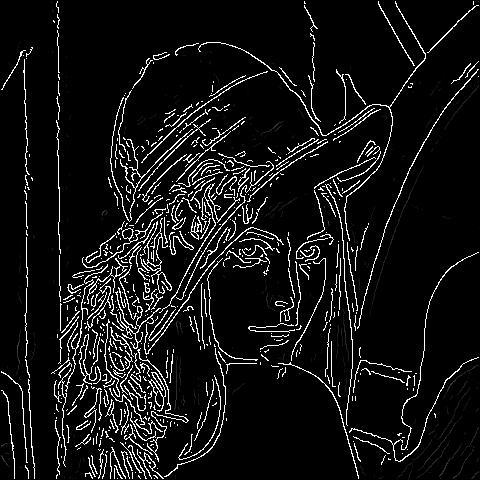
\includegraphics[width=0.5\textwidth]{images/edge_tracking.jpg}
            \caption{Εφαρμογή κατωφλίωσης με υστέρηση}
            \label{fig:thresholding-hysterisis}
        \end{figure}
    \end{itemize}
    \item \emph{Hough Transform}: Ο μετασχηματισμός Hough είναι μια ευρύτερη μέθοδος εντοπισμού χαρακτηριστικών συγκεκριμένου σχήματος μέσα σε μια εικόνα \cite{wiki:hough}. Επειδή τα επιθυμητά χαρακτηριστικά πρέπει να βρίσκονται σε κάποια παραμετρική μορφή, ο κλασσικός μετασχηματισμός Hough χρησιμοποιείται συχνά για τον εντοπισμό καμπύλων, όπως ευθείες γραμμές, κύκλοι, ελλείψεις κλπ. Τα βασικότερα πλεονεκτήματα του μετασχηματισμού αυτού είναι ότι είναι αρκετά αποτελεσματικός ακόμα και σε επικαλυπτόμενα αντικείμενα (δηλαδή είναι ανεκτικός στην έλλειψη κομματιών από μια ευθεία) και παράλληλα δεν επηρεάζεται πολύ από τον θόρυβο που υπεισέρχεται στην εικόνα. Στα πλαίσια της παρούσας διπλωματικής επιλέχθηκε η χρήση του μετασχηματισμού Hough για εντοπισμό παράλληλων γραμμών. Η βασική ιδέα της μεθόδου είναι ότι μετατρέπει τα σημεία από καρτεσιανές συντεταγμένες $(x,y)$ σε πολικές $(\rho,\theta)$ και έπειτα χρησιμοποιεί μια διαδικασία ψηφοφορίας για την ανάδειξη των υποψήφιων σχημάτων στην εικόνα.
    \begin{figure}[H]
        \centering
        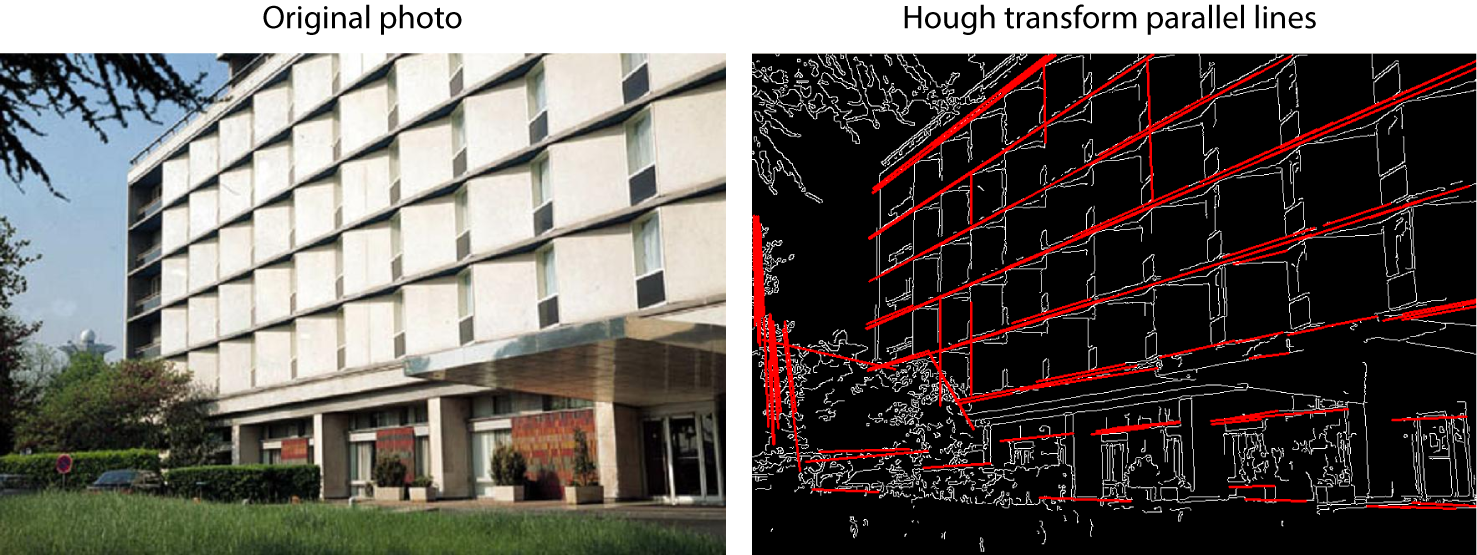
\includegraphics[width=\textwidth]{images/Hough_transform_example.png}
        \caption{Εφαρμογή Hough Transform}
        \label{fig:hough-transform-example}
    \end{figure}
\end{itemize}

\paragraph{Block-Based Recognition}\label{block-based}
Το κομμάτι του Block-Based Recognition περιλαμβάνει την προ-επεξεργασία και τον εντοπισμό παράλληλων γραμμών. Χρησιμοποιείται για να υπολογιστούν οι γωνίες των παράλληλων γραμμών και για να καταγραφούν τα σκορ κάθε pixel στα blocks.
\begin{enumerate}[1)]
    \item \emph{Προ-επεξεργασία}: Η φάση αυτή περιλαμβάνει τα εξής 4 βήματα:
    \begin{itemize}
        \item Βήμα 1: Μετατροπή του block από έγχρωμο σε κλίμακα του γκρι (grayscale), επειδή οι γραμμές της διάβασης σε μια εικόνα κλίμακας του γκρι φαίνονται ως σκούρες και φωτεινές λωρίδες.
        \item Βήμα 2: Εφαρμόζεται η μέθοδος προσαρμοστικού κατωφλίου (adaptive thresholding), η οποία αποδίδει σε ένα pixel μια δυαδική τιμή (0 ή 1) ανάλογα με το αν η τιμή του pixel είναι μεγαλύτερη από ένα μεταβλητό κατώφλι. Η διαδικασία αυτή βοηθάει να περιοριστεί το φαινόμενο της σκίασης στις εικόνες.
        \item Βήμα 3: Εφαρμογή των μορφολογικών μετασχηματισμών Διαστολής (Dilation) και Διάβρωσης (Erosion) για εξομάλυνση των ορίων.
        \item Βήμα 4: Εφαρμογή του φίλτρου Canny Edge Detector για να ανιχνευθούν οι ακμές που υπάρχουν στο block.
    \end{itemize}
    
    \item \emph{Εντοπισμός παράλληλων γραμμών}: Εφαρμόζεται ο Μετασχηματισμός Hough για να εντοπιστούν οι παράλληλες γραμμές στο block. Ορίζεται τοπικά ως αρχή των αξόνων η πάνω αριστερή γωνία του block και κάθε μη-μηδενικό pixel που ανήκει σε ακμή μετασχηματίζεται από το καρτεσιανό στο πολικό σύστημα συντεταγμένων με την παρακάτω εξίσωση:$$\rho = x\cos{\theta}+y\sin{\theta},$$ όπου η συντεταγμένη $\rho$ αναπαριστά την απόσταση της αρχής των αξόνων από την ευθεία γραμμή που διέρχεται από το $(x,y)$, και το η συντεταγμένη $\theta$ αναπαριστά την γωνία μεταξύ του κάθετου στη γραμμή διανύσματος (normal) και του άξονα x. Η αναζήτηση περιορίζεται σε παράλληλες γραμμές που βρίσκονται στο εύρος [-30\degree, +30\degree], δηλαδή ψάχνουμε μόνο για $\theta \in [60\degree,120\degree]$, επιλέγοντας διακριτές τιμές του $\theta$. Ανάλογα με τις πολικές συντεταγμένες $(\rho,\theta)$ που ικανοποιούν κάθε pixel ακμής, δημιουργείται ένας πίνακας συσσώρευσης (Σχήμα \ref{fig:voting-hough}). Το πλεονέκτημα του Block-Based Μετασχηματισμού Hough είναι ότι φιλτράρει τυχόν σημεία που έχουν υπεισέλθει στις ακμές λόγω θορύβου. Περιληπτικά, τα βήματα που ακολουθούνται για την εξαγωγή των παράλληλων γραμμών είναι τα παρακάτω:
    \begin{itemize}
        \item Βήμα 1: Σε κάθε block, ακολουθείτε μια διαδικασία ψηφοφορίας κατά την οποία κάθε ζεύγος $(\rho,\theta)$, που αντιστοιχεί σε ένα pixel ακμής, αντιστοιχίζεται σε μια θέση στον πίνακα συσσώρευσης (Σχήμα \ref{fig:voting-hough}). Κάθε φορά που ένα τέτοιο ζεύγος εντοπίζεται, η τιμή της αντίστοιχης θέσης στον πίνακα συσσώρευσης αυξάνεται κατά 1. Με άλλα λόγια κάθε pixel ακμής "ψηφίζει" για τις αντίστοιχες θέσεις (ζεύγος $(\rho,\theta)$) που ικανοποιούν την εξίσωση του. Κάθε θέση με παραπάνω από 1 ψήφους θεωρείται μια ευθεία γραμμή στις καρτεσιανές συντεταγμένες.
        \item Βήμα 2: Επιλέγονται οι 10 θέσεις με τις περισσότερες ψήφους. Η γωνία $\theta$ με τις περισσότερες ψήφους επιλέγεται ως η γωνία ανάμεσα στο κάθετο διάνυσμα της υποψήφιας παράλληλης γραμμής και του άξονα x.
        \item Βήμα 3: Εξάγονται όλες οι γραμμές των οποίων η γωνία είναι ίση με την γωνία που επιλέχθηκε στο προηγούμενο βήμα και η παραλληλία επιβεβαιώνεται εάν υπάρχουν τουλάχιστον 3 ευθείες γραμμές, των οποίων το πλήθος των ψήφων είναι μεγαλύτερο από 60.
    \end{itemize}
\end{enumerate}
\begin{figure}[H]
    \centering
    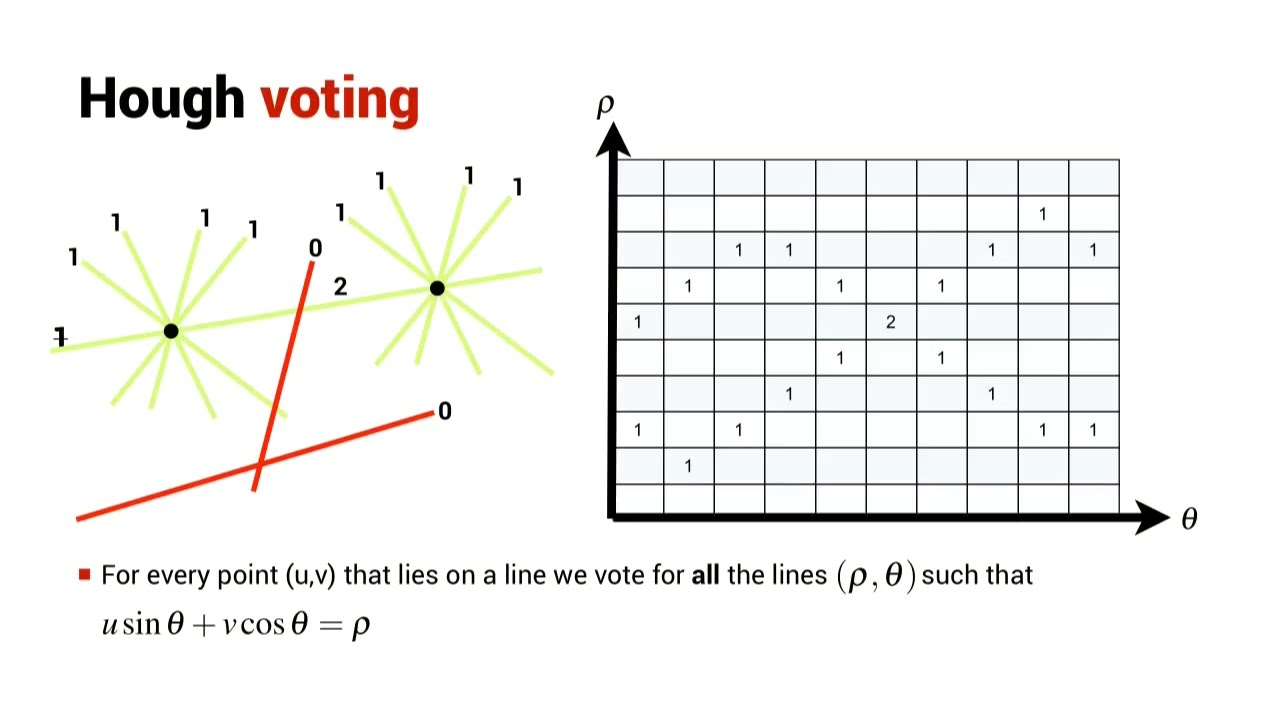
\includegraphics[width=\textwidth]{images/hough_transform.jpg}
    \caption{Παράδειγμα δημιουργίας πίνακα συσσώρευσης κατά τον μετασχηματισμό Hough \cite{FindingL66:online}. Κάθε θέση στον πίνακα εκφράζει μια ευθεία και κάθε ψήφος σε μια θέση εκφράζει τον αριθμό των σημείων από τα οποία διέρχεται αυτή η ευθεία.}
    \label{fig:voting-hough}
\end{figure}

\paragraph{Synthesize}\label{synthesize}
Αφού έχουν αναλυθεί όλα τα blocks, η τελική γωνία $\theta$ μεταξύ των παράλληλων γραμμών και του άξονα x υπολογίζεται ως αυτή με τους περισσότερους ψήφους ανά block. Τα σκορ των pixels αξιολογούνται για να εξαχθεί ένα ασφαλές μονοπάτι που να αντιστοιχεί στη διάβαση. Τα pixels με μεγαλύτερο σκορ αντιπροσωπεύουν μονοπάτι με μεγαλύτερη ασφάλεια.

\begin{figure}[H]
    \centering
    \includegraphics[width=\textwidth]{images/flow_hough_paper.jpg}
    \caption{Overview του αλγόριθμου εντοπισμού διάβασης πεζών που παρουσιάζεται στην ερευνητική εργασία \cite{wu_block-based_2019}}
    \label{fig:flow-hough-paper}
\end{figure}

\subsubsection{Αναγνώριση φωτεινού σηματοδότη}
Αν το σύστημα ανιχνεύσει διάβαση πεζών τότε καλείται ο αλγόριθμος αναγνώρισης φωτεινού σηματοδότη. Ο αλγόριθμος αυτός είναι υπεύθυνος για τον εντοπισμό του φαναριού στην εικόνα και την αναγνώριση του χρώματος (πράσινο ή κόκκινο). Η βασική ιδέα του αλγορίθμου βασίζεται στην μέθοδο του \emph{Spot Light Detection} (ανίχνευση σημειακών πηγών φωτός), η οποία εκμεταλλεύεται το γεγονός ότι οι τα φανάρια είναι αυτόφωτα, δηλαδή είναι πηγές φωτός, για να μπορέσει να εντοπίσει τη θέση τους μέσα σε μια εικόνα. Στη συνέχεια, αφού εντοπιστούν οι θέσεις της εικόνας με τους υποψήφιους φωτεινούς σηματοδότες, ορίζεται ένα bounding box (περίγραμμα) γύρω από αυτά και κάθε τέτοιο bounding box συγκρίνεται με ένα προκαθορισμένο template φωτεινού σηματοδότη. Αν το αποτέλεσμα τη σύγκρισης είναι μεγαλύτερο από ένα κατώφλι (\emph{φάση επαλήθευσης}), που ορίζεται από τον χρήστη, τότε το συγκεκριμένο bounding box, και συνεπώς η συγκεκριμένη θέση στην εικόνα, αναπαριστά έναν φωτεινό σηματοδότη. Για να γίνει αναγνώριση του κόκκινου και του πράσινου χρώματος, έχουν οριστεί δύο διαφορετικά templates που αντιπροσωπεύουν το κόκκινο και το πράσινο φανάρι.

\begin{figure}[H]
    \centering
    \includegraphics[width=\textwidth]{images/tl_system_overview.png}
    \caption{Overview του αλγόριθμου αναγνώρισης φωτεινών σηματοδοτών}
    \label{fig:tl-overview}
\end{figure}

\paragraph{Spot Light Detection}
Σκοπός του συγκεκριμένου βήματος είναι η εξαγωγή των περιοχών της αρχικής εικόνας, που είναι υποψήφιες να περιέχουν φωτεινό σηματοδότη. Η υλοποίηση του αλγορίθμου βασίστηκε σε ορισμένες ερευνητικές δημοσιεύσεις σχετικά με τον εντοπισμό φωτεινών σηματοδοτών σε εφαρμογές αυτόνομης οδήγησης \cite{de2009real, tae2006detection} και έχει την ακόλουθη δομή:
\begin{itemize}
    \item Βήμα 1: Αρχικά, όπως και στον αλγόριθμο εντοπισμού διάβασης πεζών, έτσι κι εδώ διαιρούμε την αρχική εικόνα ορίζοντας μια περιοχή ενδιαφέροντος που αντιστοιχεί στο πάνω 40\% τμήμα της αρχικής εικόνας και στο 80\% πλάτος. Αυτό συμβαίνει για να επιταχύνουμε τον αλγόριθμο, γνωρίζοντας ότι οι φωτεινοί σηματοδότες βρίσκονται σχεδόν πάντα στο πάνω κεντρικό τμήμα μιας εικόνας.
    \begin{figure}[H]
        \centering
        \includegraphics[width=0.6\textwidth]{images/upper_roi.png}
        \caption{Επιλογή περιοχής ενδιαφέροντος (ROI) για αναγνώριση φωτεινού σηματοδότη}
        \label{fig:upper-roi}
    \end{figure}
    \item Βήμα 2: Στη συνέχεια μετατρέπουμε την εικόνα από έγχρωμη σε κλίμακα του γκρι.
    \item Βήμα 3: Αφαίρεση θορύβου με εφαρμογή του \emph{μορφολογικού μετασχηματισμού Top-hat} \cite{wiki:top_hat}. Γενικά, η αρχική εικόνα μπορεί να περιέχει αρκετό θόρυβο που προέρχεται από παραμόρφωση του φακού, αντανάκλαση του ηλιακού φωτός, δόνηση της κάμερας και αντικείμενα φόντου με παρόμοιο χρώμα. Αυτός ο θόρυβος μπορεί να περιοριστεί με την εφαρμογή μορφολογικών μετασχηματισμών. Πιο συγκεκριμένα, μετασχηματισμός Top-hat ανήκει σε μια ευρύτερη οικογένεια μορφολογικών μετασχηματισμών που χρησιμοποιούν ένα δομικό στοιχείο (structuring element) το οποίο εφαρμόζεται στην αρχική εικόνα και βάσει αυτού οι τιμές των pixels αλλάζουν ανάλογα με τις τιμές των γειτονικών pixels. Γενικά το δομικό στοιχείο είναι απλού γεωμετρικού σχήματος και μεγέθους μικρότερου από το σχήμα το οποίο θα επεξεργαστεί. Υπάρχουν διάφορα σχήματα δομικών στοιχείων που μπορούν να εφαρμοστούν, τα πιο γνωστά είναι το τετράγωνο,ο σταυρός, ο δίσκος και η γραμμή. Οι μορφολογικοί τελεστές έχουν διάφορες εφαρμογές. Απλές εφαρμογές τους είναι το φιλτράρισμα, η ανίχνευση χαρακτηριστικών, η λέπτυνση, η ενίσχυση της αντίθεσης κ.α. Στην προκειμένη περίπτωση χρησιμοποιείται ένα δομικό στοιχείο σε σχήμα τετραγώνου και επιλέχθηκε ο μετασχηματισμός White Top-hat, ο οποίος επιστρέφει μια εικόνα που περιέχει τα "αντικείμενα" που είναι "μικρότερα" από το δομικό στοιχείο και πιο φωτεινά από το περιβάλλον τους. Με αυτόν τον τρόπο δίνεται έμφαση στις φωτεινές πηγές της εικόνας, όπως οι φωτεινοί σηματοδότες.
    \item Βήμα 4: Τέλος, γίνεται εξαγωγή των υποψήφιων περιοχών με χρήστη της μεθόδου Blob Detection. Ως blob ορίζεται ένα γκρουπ από συνδεδεμένα pixels που μοιράζονται κάποια κοινά χαρακτηριστικά, π.χ. έχουν την ίδια χρωματική τιμή, και στόχος της μεθόδου blob detection είναι να αναγνωρίσει και να προσδιορίσει αυτές τις περιοχές. Η OpenCV περιέχει μια κλάση, την \emph{SimpleBlobDetector}, η οποία υλοποιεί την μέθοδο Blob Detection. Ο αλγόριθμος που χρησιμοποιείται από την OpenCV, προσδιορίζει τα blobs με βάση τις παρακάτω παραμέτρους:
    \begin{itemize}
        \item Μέγεθος: φιλτράρισμα των περιοχών με βάση το εμβαδόν τους σε pixels.
        \item Circularity: παράμετρος που καθορίζει την ομοιότητα του αντικειμένου με κύκλο.
        \item Convexity: με τον όρο αυτόν εννοούμε την κυρτότητα του αντικειμένου και το φίλτρο αυτό καθορίζει τον ελάχιστο και μέγιστο βαθμό κυρτότητας.
        \begin{figure}[H]
            \centering
            \includegraphics[width=0.6\textwidth]{images/concave-convex.jpg}
            \caption{Παράδειγμα ιδιότητας convexity}
            \label{fig:convex}
        \end{figure}
        \item Inertia Ratio: αυτή η παράμετρος μετράει το πόσο επίμηκες είναι ένα αντικείμενο.
        \begin{figure}[H]
            \centering
            \includegraphics[width=0.6\textwidth]{images/inertia.jpg}
            \caption{Παράδειγμα ιδιότητας inertia ratio}
            \label{fig:inertia}
        \end{figure}
    \end{itemize}
\end{itemize}

\paragraph{Template Matching}
Template matching ονομάζεται η τεχνική εύρεσης περιοχών μιας εικόνας, που ταιριάζουν, ή είναι παρόμοιες, με μια δοθείσα εικόνα-πρότυπο. Αφού έχουν εντοπιστεί οι περιοχές που είναι υποψήφιες να περιέχουν κάποιον φωτεινό σηματοδότη, λαμβάνει χώρα το επόμενο στάδιο το οποίο περιλαμβάνει σύγκριση των περιοχών αυτών με κάποια προεπιλεγμένα templates φωτεινών σηματοδοτών. Σε αυτό το σημείο πρέπει να γίνει ξεκάθαρο ότι η σύγκριση γίνεται ανάμεσα στα πρότυπα και στην έγχρωμη αρχική εικόνα. Οι υποψήφιες περιοχές που βρέθηκαν προηγουμένως αντιστοιχούνται στην αρχική έγχρωμη εικόνα. Μετά από πειραματικές προσπάθειες βρέθηκε ότι τα templates που παρουσιάζουν μεγαλύτερη αποτελεσματικότητα είναι αυτά που φαίνονται στο σχήμα \ref{fig:templates}. Προϋπόθεση για να γίνει το template matching είναι το δοθέν πρότυπο να είναι μικρότερο σε διαστάσεις από την εικόνα προς σύγκριση. Πριν πραγματοποιηθεί η σύγκριση, εφαρμόζεται γκαουσιανό φίλτρο για την εξομάλυνση του προτύπου και το φιλτράρισμα τυχόν θορύβου. Στα πλαίσια της παρούσας διπλωματικής, στόχος ήταν να βρούμε την ομοιότητα του κόκκινου και πράσινου προτύπου με μια περιοχή της εικόνας. Αν μια υποψήφια περιοχή είχε βαθμό ομοιότητας με οποιοδήποτε πρότυπο πάνω από ένα συγκεκριμένο κατώφλι, τότε λέμε ότι αναπαριστά έναν φωτεινό σηματοδότη. Επιπλέον, συγκρίνεται η ομοιότητα με το πράσινο και το κόκκινο πρότυπο ξεχωριστά για να γίνει η αναγνώριση του χρώματος του φαναριού. Η διαδικασία ελέγχου του αποτελέσματος των συγκρίσεων με τα προκαθορισμένα κατώφλια καλείται \textbf{φάση \emph{επαλήθευσης (validation)}}.

Η σύγκριση γίνεται \emph{ολισθαίνοντας} την εικόνα-πρότυπο πάνω από την αρχική εικόνα. Με τον όρο ολίσθηση υποδηλώνεται η μετακίνηση της εικόνας-προτύπου κατά ένα pixel τη φορά (από τα αριστερά στα δεξιά, από πάνω προς τα κάτω). Σε κάθε θέση υπολογίζεται ένα μέτρο ομοιότητας που αντιπροσωπεύει το ποσοστό της ομοιότητας του προτύπου $T$ με την συγκεκριμένη περιοχή της αρχικής εικόνας $I$. Η τιμή αυτή του μέτρου για κάθε pixel αποθηκεύεται σε μια νέα εικόνα $R$, η οποία αποτελεί την εικόνα μετρήσεων (σχήμα \ref{fig:template-result}). Υπάρχουν διάφορες διαθέσιμες μέθοδοι μέτρησης της ομοιότητας \cite{Template98:online}. Στην προκειμένη περίπτωση χρησιμοποιήθηκε η μέθοδος \emph{Sum of Square Differences (SSD) Normed} η οποία υπολογίζει την ομοιότητα βάσει της παρακάτω εξίσωσης:\[R(x,y)=\frac{\sum_{x',y'}(T(x',y')-I(x+x',y+y'))^2}{\sqrt{\sum_{x',y'}T(x',y')^2\cdot \sum_{x',y'}I(x+x',y+y')^2}}\]
\begin{figure}[H]
    \centering
    \includegraphics[width=0.6\textwidth]{images/template_matching.png}
    \caption{Overview της διαδικασίας template matching}
    \label{fig:template-matching}
\end{figure}

\begin{figure}[H]
    \centering
    \includegraphics[width=0.4\textwidth]{images/template_result.png}
    \caption{Το αποτέλεσμα της διαδικασίας ολίσθησης βάσει της μετρικής Cross Correlation Normed (TM\textunderscore CCORR\textunderscore NORMED). Οι φωτεινές περιοχές υποδεικνύουν μεγαλύτερη ομοιότητα. Η θέση με τον κόκκινο κύκλο είναι αυτή με την υψηλότερη τιμή, γιαυτό η περιοχή με το περίγραμμα θεωρείται ως αυτή με το καλύτερο ταίριασμα.}
    \label{fig:template-result}
\end{figure}

\begin{figure}[H]
    \centering
    \includegraphics[width=0.5\textwidth]{images/templates.png}
    \caption{Τα templates που χρησιμοποιήθηκαν στην παρούσα εργασία}
    \label{fig:templates}
\end{figure}

\paragraph{Περισσότερα σχετικά με τους μορφολογικούς μετασχηματισμούς}
Οι μορφολογικοί μετασχηματισμοί είναι κάποιες διεργασίες που αποσκοπούν στην εξαγωγή ορισμένων χαρακτηριστικών από τις εικόνες στις οποίες εφαρμόζονται \cite{zacharia2013}. Όπως προαναφέρθηκε, σε αυτές τις διεργασίες υπάρχει ένα δομικό στοιχείο (structuring element) το οποίο είναι ουσιαστικά ένας πίνακας οποιασδήποτε διάστασης που περιέχει 0 και 1. Γενικά, το δομικό στοιχείο είναι απλού γεωμετρικού σχήματος (τετράγωνο, σταυρός, δίσκος, γραμμή) και μεγέθους μικρότερου από το σχήμα το οποίο θα επεξεργαστεί. Κάποιες από τις βασικές διεργασίες μορφολογικών μετασχηματισμών είναι οι παρακάτω \cite{OpenCVMo48:online}:
\begin{itemize}
    \item \textbf{Διαστολή (Dilation)}: Η διαστολή επεκτείνει τα αντικείμενα της εικόνας και παράλληλα κλείνει τις τρύπες που υπάρχουν. Γι' αυτό το λόγο είναι επεκτατικό φίλτρο. Αυτό που συμβαίνει είναι ότι η διαστολή τοποθετεί το δομικό στοιχείο στην εικόνα και το μετακινεί μέσα σε αυτή με τρόπο παρόμοιο με αυτόν της συνέλιξης.
    \item \textbf{Συστολή (Erosion)}: H συστολή είναι το δυαδικό συμπλήρωμα η διαστολή. Η διαδικασία που εκτελεί είναι παρόμοια με τη διαστολή, μόνο που αυτό αντί να επεκτείνει τα αντικείμενα της εικόνας, τα μικρύνει, κόβοντας παράλληλα της κορυφές των περιγραμμάτων των σχημάτων και γι' αυτό το λόγο είναι μη επεκτατικό φίλτρο.
    \item \textbf{Άνοιγμα (Opening)}: Το φίλτρο ανοίγματος αποτελεί συνδυασμό της διαστολής και της συστολής. Πιο συγκεκριμένα, υποδηλώνει μια διεργασία στην οποία ένα αντικείμενο υπόκειται πρώτα σε συστολή και αμέσως μετά σε διαστολή. Ανήκει στα μη επεκτατικά φίλτρα και χρησιμοποιείται για την αφαίρεση των μικρών αντικειμένων (που συνήθως είναι τα πιο φωτεινά) από το προσκήνιο.
    \item \textbf{Κλείσιμο (Closing)}: Αντίστοιχα, το φίλτρο κλεισίματος αποτελεί τον ανάποδο συνδυασμό από το άνοιγμα, δηλαδή πρώτα διαστολή και αμέσως μετά συστολή. Ανήκει στα επεκτατικά φίλτρα και χρησιμοποιείται για την αφαίρεση των μικρών οπών (συνήθως μαύρου χρώματος) από το προσκήνιο.
    \item \textbf{Top-Hat}: Όπως εξηγήθηκε και πιο πάνω, ο μετασχηματισμός Top-Hat χρησιμοποιείται στην επεξεργασία εικόνας για την εξαγωγή χαρακτηριστικών, την εξίσωση του φόντο, την ενίσχυση της αντίθεσης της εικόνας, την απομάκρυνση αντικειμένων από μια εικόνα κ.α. Στον Top-Hat μετασχηματισμό γίνεται είτε η αφαίρεση του αρχικού σήματος με το άνοιγμα του εαυτού του ($ I - Opening(I)$), το οποίο ονομάζεται και white Top-Hat transform, ή η αφαίρεση του κλεισίματος του σήματος με το αρχικό σήμα ($Closing(I)-I$), το οποίο ονομάζεται και ως black Top-Hat transform.
\end{itemize}
\begin{figure}[H]
    \centering
    \includegraphics[width=0.5\textwidth]{images/morph_operations.png}
    \caption{Παράδειγμα μορφολογικών διεργασιών}
    \label{fig:morph-operations}
\end{figure}

\subsubsection{Αλγόριθμος εντοπισμού εμποδίων}
Το τρίτο και τελευταίο μέρος του προτεινόμενου συστήματος πλοήγησης για άτομα με προβλήματα όρασης είναι ο αλγόριθμος εντοπισμού φυσικών εμποδίων. Ο αλγόριθμος αυτός τρέχει καθ' όλη την διάρκεια της πλοήγησης του χρήστη και χρησιμοποιεί τον ενσωματωμένο αισθητήρα βάθους της κάμερας για να αποφασίσει σχετικά με την ύπαρξη ή όχι εμποδίων μπροστά από τον χρήστη.

Η βασική ιδέα πίσω από την υλοποίηση τους συγκεκριμένου αλγόριθμου είναι αρκετά απλή. Αρχικά, λαμβάνεται η εικόνα βάθους από την κάμερα και αφού περάσει τη φάση της προ-επεξεργασίας, που αναφέραμε στην αρχή της ενότητας, εφαρμόζεται ακόμα ένα στάδιο υπο-δειγματοληψίας, με σκοπό να μειώσουμε κι άλλο το υπολογιστικό κόστος. Πιο συγκεκριμένα, οι διαστάσεις τις εικόνας μειώνονται στο μισό. Ο λόγος που εφαρμόζουμε υπο-δειγματοληψία είναι ότι στον συγκεκριμένο αλγόριθμο δεν παίζει σημαντικό ρόλο η λεπτομέρεια στην εικόνα βάθους. Το ζητούμενο είναι να εντοπιστούν μεγάλοι, ή σχεδόν μεγάλοι, όγκοι αντικειμένων μπροστά από τον χρήστη, που εμποδίζουν την διέλευσή του από το συγκεκριμένο μονοπάτι. Έτσι, η ελάττωση της λεπτομέρειας της εικόνας βάθους που επάγεται από την υπο-δειγματοληψία δεν επηρεάζει την αποτελεσματικότητα του αλγορίθμου. Τα εμπόδια που εντοπίζονται έχουν μέγιστη απόσταση από την κάμερα 1 μέτρο. Αυτό υλοποιείται εφαρμόζοντας ένα φίλτρο αποκοπής, όπου μηδενίζει όλα τα pixels που έχουν τιμή κάτω από ένα όριο, το οποίο αντιστοιχεί σε απόσταση 1μ.

Στη συνέχεια, η εικόνα διαιρείτε σε 3 υπο-περιοχές: την αριστερή, την κεντρική και την δεξιά περιοχή. Ο αλγόριθμος ελέγχει συνεχώς την κεντρική περιοχή για τυχόν εμπόδια. Αν βρεθεί εμπόδιο στην κεντρική περιοχή τότε εξετάζει την αριστερή περιοχή και αν είναι ελεύθερη από εμπόδια, ειδοποιεί τον χρήστη να μετακινηθεί προς τα αριστερά. Σε περίπτωση που υπάρχει εμπόδιο και στην αριστερή περιοχή, τότε ελέγχεται η δεξιά πλευρά και ακολούθως ο χρήστης ειδοποιείται κατάλληλα. Εάν όλες οι υπο-περιοχές είναι κατειλημμένες από εμπόδια, τότε ο αλγόριθμος φτάνει σε αδιέξοδο και περιμένει την ελευθέρωση κάποιας περιοχής. Συνήθως τέτοια εμπόδια είναι δυναμικής φύσεως, δηλαδή πρόκειται για κάποιον περαστικό, ο οποίος μετά από μερικά δευτερόλεπτα θα έχει φύγει από το οπτικό πεδίο της κάμερας κι έτσι ο αλγόριθμος θα ανακαλύψει το ελεύθερο μονοπάτι που υπάρχει. Η προτεραιότητα που δίνεται στην αριστερή περιοχή είναι καθαρά αυθαίρετη επιλογή και μπορεί κάλλιστα να τροποποιηθεί.

Η ανίχνευση των εμποδίων σε κάποια υπο-περιοχή γίνεται χρησιμοποιώντας την μέθοδο blob detection, που περιγράφηκε στην προηγούμενη ενότητα. Πιο συγκεκριμένα, η μοναδική παράμετρος που χρησιμοποιείται για την ανίχνευση εμποδίου είναι το μέγεθός του. Δεδομένου ότι η εικόνα βάθους που λαμβάνεται από την κάμερα είναι σε κλίμακα του γκρι και οι κοντινότερες περιοχές αναπαριστώνται με φωτεινότερες αποχρώσεις, η μέθοδος blob detection απομονώνει τα pixels που έχουν τιμή μεγαλύτερη από ένα συγκεκριμένο κατώφλι (π.χ. μεγαλύτερη από 100) και στη συνέχεια αναζητά ομάδες από pixels που σχηματίζουν ένα ενιαίο αντικείμενο με εμβαδόν ανάμεσα στα όρια που έχουν θεσπιστεί στον αλγόριθμο. Αν εντοπιστεί κάποιο αντικείμενο που να πληρεί τα συγκεκριμένα κριτήρια, τότε συνεπάγεται ότι αυτό είναι εμπόδιο για τον χρήστη.

\begin{figure}[H]
    \centering
    \includegraphics[width=0.8\textwidth]{images/image_division.png}
    \caption{Διαίρεση της εικόνας βάθους σε 3 τμήματα}
    \label{fig:image-division}
\end{figure}
\newpage
\begin{figure}[H]
    \centering
    \includegraphics[width=\textwidth]{images/flow_obstacle_detector.png}
    \caption{Overview αλγορίθμου εντοπισμού εμποδίων}
    \label{fig:obstacle-flow}
\end{figure}

\section{Επικοινωνία μεταξύ των συσκευών}
Σύμφωνα με την αρχιτεκτονική του προτεινόμενου συστήματος, που παρουσιάστηκε στο σχήμα \ref{fig:architecture}, απαιτείται η επικοινωνία μεταξύ του smartphone του χρήστη και της μονάδας επεξεργασίας, δηλαδή του Raspberry Pi. Το smartphone αποτελεί το μέσο παροχής ανάδρασης στον χρήστη, μέσα από το οποίο δέχεται ειδοποιήσεις σχετικά με την διαδρομή που πρέπει να ακολουθήσει, την ύπαρξη εμποδίων και την δυνατότητα διάσχισης μιας διάβασης πεζών. Επομένως, είναι απαραίτητη η διασύνδεση της επεξεργαστικής μονάδας, που υλοποιεί τους αλγορίθμους επεξεργασίας εικόνας, με την μονάδα παροχής ανάδρασης. Πιο συγκεκριμένα, το Raspberry Pi στέλνει συγκεκριμένα σήματα ελέγχου στην smartphone, τα οποία ερμηνεύονται κατάλληλα από την εφαρμογή Android και μεταφράζονται στα αντίστοιχα μοτίβα δονήσεων.

\subsection{Απαιτήσεις συστήματος}
Η βασική προϋπόθεση είναι η ασύρματη επικοινωνία, η οποία να επιτρέπει την αμφίδρομη αποστολή/λήψη μηνυμάτων από τις δύο πλευρές. Η κύρια ροή μηνυμάτων είναι από το Raspberry Pi προς το smartphone, ωστόσο είναι αναγκαία και η αντίστροφη διαδρομή, από το smartphone προς το Raspberry Pi, για την λήψη μηνυμάτων επιβεβαίωσης (confirmation messages).

Η αρχική σκέψη του συγγραφέα ήταν η υλοποίηση μιας αμφίδρομης σύνδεσης Bluetooth μεταξύ των δύο συσκευών. Κάτι τέτοιο αποδείχθηκε αρκετά προβληματικό, ωστόσο, αφού τόσο τόσο το Raspberry Pi 4 όσο και το smartphone χρησιμοποιούσαν το πρωτόκολλο Bluetooth 5, το οποίο είναι αρκετά δύσχρηστο για περιπτώσεις όπου χρειάζεται η υλοποίηση μιας απλής σύνδεσης. Επιπλέον, η ξεχωριστή υλοποίηση της Bluetooth σύνδεσης τόσο σε C++ (Raspberry Pi) όσο και σε Java (Android App), αποδείχθηκε πολύ χρονοβόρα, οπότε απορρίφθηκε η λύση του Bluetooth. Η εναλλακτική που επιλέχθηκε ήταν η χρήση του \emph{δικτυακού προγραμματισμού (socket programming)}.

\subsection{Socket Communication}
Η υλοποίηση μιας ασύρματης σύνδεσης με χρήση των λεγόμενων sockets απαιτεί την ύπαρξη ενός τοπικού δικτύου, στο οποίο να είναι συνδεδεμένες οι συσκευές που πρόκειται να επικοινωνήσουν. Για την εγκαθίδρυση ενός τοπικού δικτύου συνδέουμε και τις δύο συσκευές (smartphone \& raspberry pi) σε ένα δίκτυο Wifi. Για τις ανάγκες της διπλωματικής εργασίας οι δύο συσκευές συνδέθηκαν σε ένα δίκτυο wifi-hotspot που παρεχόταν από ένα τρίτο smartphone. Μέσω του ίδιου δικτύου οι συσκευές είχαν πρόσβαση στο διαδίκτυο. Παρακάτω αναλύεται περισσότερο η δομή μιας σύνδεσης μέσω sockets \cite{wiki:sockets}.

\subsubsection{Sockets}
Τα sockets (ή αλλιώς \emph{υποδοχές} στα ελληνικά) παρέχουν σημειακή, αμφίδρομη επικοινωνία μεταξύ διεργασιών, συνήθως -αλλά όχι απαραίτητα- μέσω δικτύου. Αποτελούν μια πολύ ευέλικτη και θεμελιώδη μέθοδο δικτυακής επικοινωνίας μεταξύ διεργασιών ή συστημάτων. Ένα socket είναι μια τερματική σύνδεση η οποία μπορεί να λάβει ένα όνομα (name). Επίσης έχει ένα τύπο (type) και σχετίζεται με μια ή περισσότερες διεργασίες. Τα sockets, ανάλογα με την εφαρμογή που εξυπηρετούν, χαρακτηρίζονται από ένα πρωτόκολλο. Όταν τα sockets χρησιμοποιούνται για επικοινωνία μέσω ενός δικτύου, όπως το internet, αξιοποιούν το πρωτόκολλο επικοινωνίας TCP/IP. Η διεύθυνση ενός socket στο internet αποτελείται από μια διεύθυνση IP και έναν αριθμό θύρας (port).

\subsubsection{Τύποι sockets: TCP/UDP}
Για να γίνει επικοινωνία μεταξύ δύο τερματικών σημείων (endpoints) πρέπει αυτά να χρησιμοποιούν sockets του ίδιου τύπου. Οι δύο βασικοί και πιο διαδεδομένοι τύποι sockets είναι οι ακόλουθοι:
\begin{itemize}
    \item \emph{Stream socket}: Παρέχει αμφίδρομη, ακολουθιακή, αξιόπιστη και μη-επαναλαμβανόμενη ροή δεδομένων χωρίς καθορισμένα όρια μηνύματος. Η επικοινωνία μοιάζει με τηλεφωνική επικοινωνία και χρησιμοποιεί το πρωτόκολλο TCP.
    \item \emph{Datagram socket}: Υποστηρίζει αμφίδρομη ροή μηνυμάτων (datagrams). Η σειρά αποστολής και παραλαβής μηνυμάτων μπορεί να μην είναι  ακολουθιακή. Τα όρια των μηνυμάτων είναι καθορισμένα. Η επικοινωνία μοιάζει με ανταλλαγή επιστολών μέσω ταχυδρομείου και χρησιμοποιεί το πρωτόκολλο UDP.
\end{itemize}
Η σύνδεση που υλοποιήθηκε στα πλαίσια της διπλωματικής χρησιμοποιεί τα stream sockets, που βασίζονται στο TCP, επειδή είναι αναγκαία η αξιόπιστη και μη-επαναλαμβανόμενη μετάδοση των σημάτων ελέγχου από το Raspberry Pi προς το smartphone.

\subsection{Server/Client}
Η επικοινωνία ακολουθεί το μοντέλο εξυπηρετητή/πελάτη (server/client), δηλαδή το ένα τερματικό σημείο λειτουργεί ως εξυπηρετητής και είναι υπεύθυνο για την δημιουργία της σύνδεσης, ενώ το άλλο λειτουργεί ως πελάτης και συνδέεται στην σύνδεση που έχει δημιουργηθεί από έναν εξυπηρετητή. Είναι δυνατόν να υπάρχουν πολλοί διαφορετικοί πελάτες που συνδέονται στον ίδιο εξυπηρετητή και αφού εγκαθιδρυθεί η σύνδεση, τότε η επικοινωνία γίνεται και προς τις δύο πλευρές. Μια σύνδεση μέσω sockets μπορεί να τερματιστεί και από τις δύο πλευρές.

\subsubsection{Server}
Τον ρόλο του server λαμβάνει το Raspberry Pi, δηλαδή είναι υπεύθυνο για την δημιουργία της σύνδεσης. Τα βήματα που υλοποιεί ένας server για τη σύνδεση είναι τα εξής:
\begin{enumerate}
    \item Δημιουργεί ένα socket.
    \item Δεσμεύει το socket με την επιθυμητή δικτυακή διεύθυνση του τελικού σημείου.
    \item Ζητά από το λειτουργικό σύστημα να “ακούει” για εισερχόμενες συνδέσεις.
    \item Εισέρχεται σε κατάσταση όπου αναμένει διαρκώς να του παραδώσει μια σύνδεση το λειτουργικό σύστημα.
    \item Αν λάβει αίτημα εισερχόμενης σύνδεσης, τότε στέλνει πίσω μήνυμα επιβεβαίωσης και δημιουργεί την σύνδεση.
\end{enumerate}

\subsubsection{Client}
Τον ρόλο του μοναδικού client παίζει το smartphone του χρήστη με την εγκατεστημένη εφαρμογή Android. Τα βήματα που ακολουθεί ο client για να συνδεθεί σε ένα socket είναι τα εξής:
\begin{enumerate}
    \item Δημιουργεί ένα socket.
    \item Επιλέγει την διεύθυνση IP του server και προσδιορίζει την επιθυμητή θύρα (port).
    \item Υποβάλλει αίτηση σύνδεσης στον server.  
    \item Με το που λάβει το μήνυμα επιβεβαίωσης εγκαθιδρύεται η σύνδεση.
\end{enumerate}

\begin{figure}[H]
    \centering
    \includegraphics[width=\textwidth]{images/socket_client_server.png}
    \caption{Μοντέλο Server/Client για μια σύνδεση TCP μέσω sockets}
    \label{fig:client-server}
\end{figure}

\clearemptydoublepage
\chapter{Πειραματικός Έλεγχος Συστήματος} \label{ch:demo}
\markboth{Πειραματικός Έλεγχος Συστήματος}{}

Στην ενότητα αυτή παρουσιάζονται μερικά αποτελέσματα που αφορούν τον πειραματικό έλεγχο ορθής λειτουργίας του συστήματος πλοήγησης που προτάθηκε. Αρχικά, πρέπει να το τονιστεί το γεγονός πως οι χρονικοί περιορισμοί της διπλωματικής εργασίας δεν επέτρεψαν την διενέργεια ενός επίσημου τεστ χρηστικότητας σε πραγματικούς χρήστες με προβλήματα όρασης. Παρόλα αυτά έγινε μια προσπάθεια ελέγχου κάθε ξεχωριστού τμήματος της διπλωματικής πριν την ενσωμάτωσή του στο υπόλοιπο σύστημα, όπως επίσης και συνολικός έλεγχος ολόκληρου του συστήματος. Για την πληρέστερη περιγραφή έγινε καταγραφή ενός βίντεο επίδειξης (demo), στο οποίο παρουσιάζονται οι δυνατότητες του υλοποιηθέντος συστήματος πλοήγησης. Το βίντεο μπορείτε να το βρείτε στο ακόλουθο λινκ \url{https://youtu.be/2TiHW27NSLQ}.

\section{Απόδοση αλγορίθμων}
Κάθε αλγόριθμος που παρουσιάστηκε στην ενότητα της υλοποίησης δοκιμάζεται και ελέγχεται κατά πόσο λειτουργεί αποτελεσματικά και σύμφωνα με τις προδιαγραφές που ορίστηκαν. Είναι σημαντικό να τονίσουμε ότι, αν και στην αρχή το πρόγραμμα είχε πολύ χαμηλά fps (frames per second), μετά από κατάλληλες τροποποιήσεις στον κώδικα και στην λογική των αλγορίθμων η ταχύτητα κυμαίνεται στο εύρος 20-30fps, το οποίο είναι ένα πολύ καλό νούμερο για εφαρμογές πραγματικού χρόνου.

\subsection{Εντοπισμός διάβασης πεζών}
Ο αλγόριθμος εντοπισμού διαβάσεων λειτουργεί αρκετά αποτελεσματικά κάτω από φυσιολογικές συνθήκες φωτισμού και τα πάει αρκετά καλά ακόμα και σε πιο ακραίες συνθήκες, όπως βρεγμένος δρόμος ή αντανακλάσεις από τον ήλιο. Είναι γεγονός πως σε συνθήκες πολύ χαμηλού φωτισμού, όπως π.χ. όταν επικρατεί σκοτάδι, δεν μπορεί να λειτουργήσει αποδοτικά. Παρακάτω, παρατίθενται παραδείγματα διαβάσεων που αναγνωρίζονται από τον προτεινόμενο αλγόριθμο, καθώς και μερικές περιπτώσεις στις οποίες "εξαπατάται" από το οπτικό περιβάλλον, όπως για παράδειγμα στην ύπαρξη σκαλιών.
\begin{figure}[H]
    \centering
    \includegraphics[width=\textwidth]{images/test_zebra1.png}
    \caption{Παράδειγμα εντοπισμού διάβασης πεζών. Η γκρίζα ευθεία γραμμή πάνω στη διάβαση, καθώς και η λευκή περιοχή κάτω από την διάβαση υποδηλώνουν το βέλτιστο μονοπάτι που πρέπει να ακολουθήσει ο χρήστης. Επίσης, το πρόγραμμα εμφανίζει και την κλίση των γραμμών της διάβασης σε μοίρες. Απλή διάβαση (αριστερά), βρεγμένη διάβαση (δεξιά).}
    \label{fig:test-zebra1}
\end{figure}
\begin{figure}[H]
    \centering
    \includegraphics[width=\textwidth]{images/test_zebra3.png}
    \caption{Παράδειγμα εντοπισμού διάβασης πεζών με παρουσία εμποδίων (αριστερά) ή αντανάκλασης ηλιακού φωτός (δεξιά)}
    \label{fig:test-zebra3}
\end{figure}
\begin{figure}[H]
    \centering
    \includegraphics[width=\textwidth]{images/test_zebra2.png}
    \caption{Παράδειγμα εντοπισμού διάβασης πεζών άλλων χρωματικών αποχρώσεων (αριστερά) ή σε σκοτεινό περιβάλλον (δεξιά)}
    \label{fig:test-zebra2}
\end{figure}
\subsection{Αναγνώριση φωτεινού σηματοδότη}
Ο αλγόριθμος αναγνώρισης φωτεινού σηματοδότη λειτουργεί επαρκώς καλά κάτω από συγκεκριμένες συνθήκες. Η αποτελεσματικότητά του επηρεάζεται άμεσα από την ένταση της φωτεινότητας του φαναριού, την ανάλυση της κάμερας, την γωνία λήψης της φωτογραφίας και τις εξωτερικές συνθήκες περιβάλλοντος, π.χ. συννεφιά, βροχή κλπ. Ωστόσο, η χρήση του κάτω από συνηθισμένες συνθήκες δίνει ικανοποιητικά αποτελέσματα.
\begin{figure}[H]
    \centering
    \includegraphics[width=0.9\textwidth]{images/test_light1.png}
    \caption{Παράδειγμα αναγνώρισης κόκκινου φωτεινού σηματοδότη (κόκκινο περίγραμμα γύρω από το φανάρι). Οι μπλε κύκλοι υποδηλώνουν πιθανές περιοχές με φωτεινό σηματοδότη που εντοπίστηκαν από τον αλγόριθμο, αλλά δεν πέρασαν τη φάση της επικύρωσης (validation). Τα νούμερα που φαίνονται αριστερά στην κονσόλα είναι η τιμή του μέτρου σύγκρισης κατά την εφαρμογή του template matching.}
    \label{fig:test-light1}
\end{figure}
\begin{figure}[H]
    \centering
    \includegraphics[width=0.9\textwidth]{images/test_light2.png}
    \caption{Παραδείγματα αναγνώρισης κόκκινου φωτεινού σηματοδότη (κόκκινο περίγραμμα γύρω από το φανάρι).}
    \label{fig:test-light2}
\end{figure}
\begin{figure}[H]
    \centering
    \includegraphics[width=0.9\textwidth]{images/test_light3.png}
    \caption{Παράδειγμα αναγνώρισης πράσινου φωτεινού σηματοδότη (πράσινο περίγραμμα γύρω από το φανάρι).}
    \label{fig:test-light3}
\end{figure}
\begin{figure}[H]
    \centering
    \includegraphics[width=0.9\textwidth]{images/test_light4.png}
    \caption{Παραδείγματα αναγνώρισης πράσινου φωτεινού σηματοδότη (πράσινο περίγραμμα γύρω από το φανάρι). Οι μπλε κύκλοι υποδηλώνουν πιθανές περιοχές με φωτεινό σηματοδότη που εντοπίστηκαν από τον αλγόριθμο, αλλά δεν πέρασαν τη φάση της επικύρωσης (validation). Τα νούμερα που φαίνονται αριστερά στην κονσόλα είναι η τιμή του μέτρου σύγκρισης κατά την εφαρμογή του template matching.}
    \label{fig:test-light4}
\end{figure}

\subsection{Αποφυγή εμποδίων}
Ο αλγόριθμος αποφυγής εμποδίων είναι ο πιο απλός αλγόριθμος του συστήματος. Λειτουργεί αποτελεσματικά στις περισσότερες περιπτώσεις, ενώ είναι ιδιαίτερα ανθεκτικός σε συνθήκες φωτισμού και εξωτερικού περιβάλλοντος.

\begin{figure}[H]
    \centering
    \includegraphics[width=0.8\textwidth]{images/test_depth_clear.png}
    \caption{Παράδειγμα εντοπισμού εμποδίων. Η κεντρική περιοχή της εικόνας βάθους είναι κενή, άρα το σύστημα ειδοποιεί τον χρήστη να προχωρήσει ελεύθερα.}
    \label{fig:test-depth-clear}
\end{figure}
\begin{figure}[H]
    \centering
    \includegraphics[width=0.7\textwidth]{images/test_depth_left.png}
    \caption{Παράδειγμα εντοπισμού εμποδίων. Η κεντρική περιοχή της εικόνας βάθους είναι κατειλημμένη από εμπόδιο, άρα το σύστημα ειδοποιεί τον χρήστη να μετακινηθεί αριστερά στον κενό χώρο.}
    \label{fig:test-depth-left}
\end{figure}
\begin{figure}[H]
    \centering
    \includegraphics[width=0.7\textwidth]{images/test_depth_right.png}
    \caption{Παράδειγμα εντοπισμού εμποδίων. Τόσο η κεντρική, όσο και η αριστερή περιοχή της εικόνας βάθους είναι κατειλημμένες από εμπόδια, άρα το σύστημα ειδοποιεί τον χρήστη να μετακινηθεί δεξιά στον κενό χώρο.}
    \label{fig:test-depth-right}
\end{figure}

\section{Απτική ανάδραση}
Η χρήση απτικής ανάδρασης για την ειδοποίηση του χρήστη είναι από τα πιο δυνατά χαρακτηριστικά του συστήματος. Παρέχει διακριτικότητα και δίνει στον χρήστη την άνεση να μετακινείται στον χώρο χωρίς να απαιτείται η χρήση κάποιου ακουστικού. Τα μοτίβα δονήσεων (haptic icons), όπως παρουσιάστηκαν στην ενότητα 3.4.4, είναι ευδιάκριτα μεταξύ τους χάρη στον περιορισμένο αριθμό τους και στην χρήση κατάλληλων συνδυασμών παύσης, δόνησης και έντασης σε κάθε ξεχωριστό μοτίβο. Το γεγονός αυτό καθιστά την εκμάθησή τους εύκολη και γρήγορη, ενώ αναδεικνύεται η καταλληλότητά τους για ένα σύστημα πλοήγησης για άτομα με προβλήματα όρασης.

\section{Τελική διάταξη}
Η τελική διάταξη του πειραματικού συστήματος περιλαμβάνει την ενσωμάτωση όλου του εξοπλισμού (Raspberry Pi 4, Camera, Powerbank) σε ένα τσαντάκι μέσης, που λειτουργεί ως μέσο στήριξης, για την εύκολη και άνετη χρήση του από το άτομο με προβλήματα όρασης. Στο σχήμα \ref{fig:final-version} φαίνεται η τελική μορφή του συστήματος πάνω στον χρήστη. Ο χρήστης, πέρα από το τσαντάκι μέσης με τον εξοπλισμό, κρατάει και το smartphone από το οποίο δέχεται ανάδραση.

\begin{figure}[H]
    \centering
    \includegraphics[width=\textwidth]{images/final-version.png}
    \caption{Τελική διάταξη προτεινόμενου συστήματος}
    \label{fig:final-version}
\end{figure}
\clearemptydoublepage
\chapter{Συμπεράσματα - Προτάσεις για το μέλλον} \label{ch:conclusion}
\markboth{Συμπεράσματα}{}

Στην ενότητα αυτή παρουσιάζονται συνοπτικά τα πλεονεκτήματα και τα μειονεκτήματα του συστήματος πλοήγησης που προτείνεται στην εργασία μας. Παράλληλα, προτείνονται ορισμένες βελτιώσεις που αφορούν κάποια χαρακτηριστικά του συστήματος με σκοπό την συνολική αύξηση της απόδοσης, αλλά και της χρηστικότητάς του. Στόχος της παρούσας διπλωματικής εργασίας ήταν η υλοποίηση ενός διακριτικού συστήματος πλοήγησης για άτομα με προβλήματα όρασης, το οποίο θα υποβοηθούσε τον χρήστη να διασχίζει τους δρόμους και να μετακινείται με περισσότερη άνεση και ασφάλεια μέσα σε ένα αστικό περιβάλλον με παράλληλη χρήση του λευκού μπαστουνιού. Ο στόχος αυτός επετεύχθη και, παρ' όλες τις ατέλειες του συστήματος, η τελική πειραματική υλοποίησή του είναι λειτουργική και έρχεται πολύ κοντά στις αρχικές φιλοδοξίες του συγγραφέα.

\section{Πλεονεκτήματα}
Το κύριο πλεονέκτημα του συστήματος είναι η ενσωμάτωση διαφορετικών λειτουργιών και η φορητότητά του. Πιο συγκεκριμένα, συνδυάζει τρία επίπεδα καθοδήγησης, την πλοήγηση turn-by-turn, την αποφυγή εμποδίων και την υποβοήθηση διάσχισης διάβασης πεζών. Οι τρεις αυτές λειτουργίες παρέχονται ταυτόχρονα στον χρήστη καθ' όλη την διάρκεια πλοήγησής του. Επιπλέον, το σύστημα χαρακτηρίζεται από διακριτικότητα όσον αφορά τον όγκο του εξοπλισμού που χρησιμοποιεί και ελάχιστη επεμβατικότητα στις συνήθειες και τη συμπεριφορά του χρήστη, καθώς όλα τα μέρη ενσωματώνονται σε ένα τσαντάκι μέσης.

Παράλληλα, η υλοποίηση που προτείνεται είναι αρκετά φιλική προς τον χρήστη και υποστηρίζει την ελάχιστη παρεμβατικότητα, ενώ αξιοποιεί την λογική plug-and-play, δηλαδή ο χρήστης απλά φοράει το τσαντάκι μέσης και ενεργοποιεί το σύστημα μέσω του κινητού του, χωρίς να χρειάζεται περαιτέρω ρύθμιση. Η χρήση των μοτίβων δονήσεων (haptic icons) είναι αρκετά απλή και κατανοητή, μιας και ο αριθμός τους είναι μικρός, μόλις 4 διαφορετικά μοτίβα, και η διαδικασία εκμάθησής τους γρήγορη και εύκολη.

\section{Μειονεκτήματα}
Στα πλαίσια εκπόνησης μιας διπλωματικής εργασίας δεν υπάρχει ο απαραίτητος χρόνος για την υλοποίηση ενός πλήρους και ολοκληρωμένου συστήματος πλοήγησης που θα λειτουργεί απρόσκοπτα χωρίς προβλήματα. Παρόλο, λοιπόν, που το προτεινόμενο σύστημα είναι λειτουργικό, παρουσιάζει όπως είναι φυσικό ορισμένα μειονεκτήματα τα οποία είναι κυρίως αλγοριθμικής φύσεως. Από την άλλη πλευρά, το μοναδικό ίσως μειονέκτημα δομικής φύσεως είναι η χαμηλή απόδοση του συστήματος σε συνθήκες νύχτας, μιας και βασίζεται στην χρήση κάμερας και η ύπαρξη φωτισμού είναι αναγκαία.

\subsection{Ανίχνευση διάβασης πεζών}
Καταρχάς, ο αλγόριθμος ανίχνευσης διάβασης πεζών φαίνεται να είναι επιρρεπής στις περιβαλλοντικές συνθήκες, στις συνθήκες του οδοστρώματος (βρεγμένο ή όχι), ενώ εξαρτάται επίσης και από τον βαθμό συντήρησης της διάβασης πεζών (κατά πόσο έντονη είναι η διαγράμμιση). Μετά από κάποιες δοκιμές, ωστόσο, βρέθηκε ότι η μεγαλύτερη αδυναμία του συγκεκριμένου αλγορίθμου είναι η παραπλάνησή του από εικόνες που περιέχουν σκαλοπάτια, αντί για διάβαση πεζών. Εξαιτίας του γεγονότος ότι αξιοποιείται το εναλλασσόμενο μοτίβο των δύο γραμμών για την αναγνώριση της διάβασης, ο αλγόριθμος βγάζει λάθος συμπεράσματα όταν επεξεργάζεται φωτογραφίες που απεικονίζουν σκαλοπάτια, μιας και οι τελευταίες ενσωματώνουν περίπου το ίδιο εναλλασσόμενο μοτίβο, όπως φαίνεται στο σχήμα \ref{fig:test-zebra4}.

\begin{figure}[H]
    \centering
    \includegraphics[width=\textwidth]{images/test_zebra4.png}
    \caption{Παράδειγμα παραπλάνησης αλγορίθμου. Το πρόγραμμα αναγνωρίζει λανθασμένα κάποια σκαλοπάτια ως διάβαση πεζών. Αυτό συμβαίνει επειδή τα μοτίβα των σκαλοπατιών και της διάβασης είναι παρόμοια μεταξύ τους.}
    \label{fig:test-zebra4}
\end{figure}

\subsection{Αναγνώριση φωτεινού σηματοδότη}
Όσον αφορά τον αλγόριθμο αναγνώρισης φωτεινού σηματοδότη, η βασική του αδυναμία έγκειται στο γεγονός πως το τελικό αποτέλεσμα εξαρτάται σε πολύ μεγάλο ποσοστό από τον τύπο των templates που χρησιμοποιούνται για την αντιστοίχηση του χρώματος του φαναριού. Τέλος, η φύση του αλγορίθμου αυτού τον καθιστά αρκετά ευάλωτο στις περιβαλλοντικές συνθήκες φωτισμού. Σχετικό παράδειγμα παρουσιάζεται στο σχήμα \ref{fig:test-light5}.

\begin{figure}[H]
    \centering
    \includegraphics[width=\textwidth]{images/test_light5.png}
    \caption{Παράδειγμα αστοχίας αλγορίθμου. Το πρόγραμμα αναγνωρίζει λανθασμένα κάποια σημεία της εικόνας ως φανάρια και τα ερμηνεύει με κόκκινο χρώμα. Αυτό συμβαίνει επειδή υπάρχουν έντονες αντανακλάσεις του ηλιακού φωτός, ενώ αντίστοιχα η ένταση της φωτεινότητας του φαναριού είναι χαμηλή.}
    \label{fig:test-light5}
\end{figure}

\section{Μελλοντικές προτάσεις}
Οι παρακάτω προτάσεις αφορούν την βελτίωση ορισμένων χαρακτηριστικών του συστήματος τα οποία θα αυξήσουν άμεσα την απόδοση και την αποτελεσματικότητά του και τα οποία δεν μπόρεσαν να υλοποιηθούν, κυρίως, λόγω έλλειψης χρόνου.

\subsection{Μετατροπέας Voice-to-Text}
Μια αναγκαία προσθήκη που απαιτείται για να κάνει το παραπάνω σύστημα πλήρως προσβάσιμο σε άτομα με προβλήματα όρασης είναι η ενσωμάτωση ενός μετατροπέα φωνής σε κείμενο (Voice-to-Text) και, αντίστροφα, κειμένου σε φωνή (Text-to-Voice). Με τον τρόπο αυτό ο χρήστης θα μπορεί να πλοηγείται στην εφαρμογή πλήρως ανεξάρτητα, ενώ η εισαγωγή του προορισμού θα γίνεται μέσω φωνητικών εντολών του χρήστη. Για την υλοποίηση του τελευταίου, υπάρχει ήδη διαθέσιμο Google API για android development που χρησιμοποιεί τον αλγόριθμο αναγνώριση φωνής της Google.

\subsection{Αναγνώριση εμποδίων}
Δεύτερη σημαντική προσθήκη είναι η βελτίωση του υπάρχοντος αλγορίθμου εντοπισμού εμποδίων. Πιο συγκεκριμένα, για να είναι πιο αποδοτικός θα πρέπει να χρησιμοποιεί πιο εξελιγμένη λογική στην ανάλυση της εικόνας βάθους και να ενσωματώνει λειτουργία αναγνώρισης του είδους των εμποδίων που ανιχνεύονται, π.χ. άνθρωπος, κολόνα, αυτοκίνητο κλπ.

\subsection{Βελτιωμένο template φωτεινού σηματοδότη}
Ο αλγόριθμος αναγνώρισης φωτεινού σηματοδότη βασίζεται στην χρήση ενός συγκεκριμένου προτύπου. Ένας τρόπος να αυξήσουμε την απόδοση του αλγορίθμου αυτού είναι να βρεθεί ένα καλύτερο πρότυπο, το οποίο να αντιπροσωπεύει πιο αποτελεσματικά τους φωτεινούς σηματοδότες. Κάτι τέτοιο απαιτεί αντίστοιχη έρευνα για την εξακρίβωση των χαρακτηριστικών εκείνων που παίζουν μεγαλύτερο ρόλο στο template matching.

\subsection{Αυτονομία}
Η αυτονομία ενός συστήματος πλοήγησης είναι ένα από τα κύρια χαρακτηριστικά που ενδιαφέρει τον τελικό χρήστη, καθώς έχει ανάγκη την, όσο το δυνατόν, μεγαλύτερη διάρκεια συνεχόμενης χρήσης.
Η αυτονομία του συστήματος εξαρτάται τόσο από το μέγεθος της φορητής μπαταρίας (powerbank) όσο και από την κατανάλωση του συστήματος. Θεωρώντας δεδομένη την κατανάλωση, θα προτείναμε να γίνει χρήση μιας μεγαλύτερης σε χωρητικότητα μπαταρίας, η οποία θα επιτρέπει την συνεχόμενη χρήση τουλάχιστον 2 ωρών. Για τις ανάγκες της διπλωματικής εργασίας, η αυτονομία της πειραματικής διάταξης ήταν παραπάνω από αρκετή.

\subsection{Usability test}
Τέλος, κάθε σύστημα που προορίζεται για χρήση από τελικούς χρήστες είναι απαραίτητο να περνάει από έναν έλεγχο χρηστικότητας (usability test). Συνήθως ο έλεγχος αυτός περιλαμβάνει την χρήση του προς εξέταση συστήματος από τους πραγματικούς χρήστες, δηλαδή από άτομα που πάσχουν από προβλήματα μειωμένης όρασης, και υπάρχουν διάφορες μέθοδοι που μπορούν να αξιοποιηθούν για τον υπολογισμό μιας μετρικής χρηστικότητας, όπως είναι οι 10 ευρετικοί κανόνες του Nielsen \cite{nielsen1990}.
\clearemptydoublepage
\chapter{Παράρτημα} \label{ch:appendix}
\markboth{Παράρτημα}{}

\section{Φωτογραφίες εξοπλισμού}
\begin{figure}[H]
    \centering
    \includegraphics[width=0.7\textwidth]{images/equipment1.png}
    \caption{Η κάμερα Intel Realsense 435i (πάνω) και το Powerbank Intenso PD10000 (κάτω)}
    \label{fig:equipment1}
\end{figure}

\begin{figure}[H]
    \centering
    \includegraphics[width=0.8\textwidth]{images/equipment2.png}
    \caption{Το Raspberry Pi 4 χωρίς θήκη (πάνω) και με προστατευτική θήκη (μέση) και τσαντάκι μέσης με όλο τον εξοπλισμό μέσα (κάτω)}
    \label{fig:equipment2}
\end{figure}
\clearemptydoublepage
% Next Chapters
% .............
% .............

%**************************%
%    END OF MAIN THESIS    %
%**************************%
% bibliography
\bibliographystyle{IEEEtran}
\bibliography{IEEEabrv, library/bibliography.bib}
\clearemptydoublepage
% Last Page
\pagestyle{empty}

\vspace*{\fill}
\noindent \hspace{2cm} \rule{12.7cm}{0.4pt}\\
\vspace{-1.7em}
\begin{flushleft}
	\hspace*{30mm}Πανεπιστήμιο Πατρών, Πολυτεχνική Σχολή\\
	\hspace*{30mm}Τμήμα Ηλεκτρολόγων Μηχανικών \& Τεχνολογίας Υπολογιστών\\
	\hspace*{30mm}{\nomme}\\
	\hspace*{30mm}© \monthyear \ -- Με επιφύλαξη παντός δικαιώματος\\
\end{flushleft}
\vspace{-1.2em}
\noindent \hspace{2cm} \rule{12.7cm}{0.4pt}

\end{document}
